\documentclass[12pt]{article}

\RequirePackage[OT1]{fontenc}
\RequirePackage{amsthm,amsmath}
\RequirePackage{natbib}
\RequirePackage{hyperref}
\usepackage{enumerate} 
\usepackage{graphicx}
\usepackage{amsfonts}
\usepackage{bm,bbm} 
\usepackage[]{algorithm2e}
\usepackage{epstopdf}
\usepackage{caption}
\usepackage{subcaption}
\RequirePackage{color}

\usepackage{multirow}

% settings
%\pubyear{2005}
%\volume{0}
%\issue{0}
%\firstpage{1}
%\lastpage{8}
%\arxiv{arXiv:0000.0000}


\usepackage{color}
\newcommand{\jessi}[1]{{\color{blue}[[\textbf{Jessi: }#1]]}}

\RequirePackage{bm}

\usepackage[font = {it}]{caption}
\newcommand{\reels}{\mathbb R}
\newcommand{\Proba}{\rm{Pr}}
\newcommand{\Expa}{\mathbb E}
\newcommand{\ints}{\mathbb Z}
\newcommand{\mbf}{\mathbf}
\newcommand{\indic}{\mathbbm{I}}
%\newcommand{\bm}{\boldmath}
\newcommand{\Msun}{M_{\odot}}
\newcommand{\note}{\textcolor{red}}

\newcommand{\btheta}{\boldsymbol{\theta}}
\newcommand{\x}{{\bf x}}
\newcommand{\cvert}{{\hspace{.01in}\vert\hspace{.01in}}}
\newcommand{\locdist}{\Delta}
\newcommand{\I}{\mbox{\Large {\bf 1}}}
\renewcommand{\L}{{\cal L}}
\newcommand{\E}{\mathbb{E}}
\renewcommand{\Re}{\mathbb{R}}


\newcommand{\boldeta}{\boldsymbol{\eta}}
\newcommand{\s}{{\bf s}}

\newcommand{\msim}{m_{\text{sim}}}
\newcommand{\mobs}{m_{\text{obs}}}

\newcommand{\nsim}{n_{\text{sim}}}
\newcommand{\nobs}{n_{\text{obs}}}

\newcommand{\Cmin}{C_{\text{min}}}
\newcommand{\Cmax}{C_{\text{max}}}

\newcommand{\Mtot}{M_{\text{tot}}}

\newcommand{\Mmax}{M_{\text{max}}}
\newcommand{\Mmin}{M_{\text{min}}}

% NOTE: To produce *un*blinded version, replace "0" with "1" below.
\newcommand{\blind}{1}

% DON'T change margins - should be 1 inch all around.
\addtolength{\oddsidemargin}{-.5in}%
\addtolength{\evensidemargin}{-.5in}%
\addtolength{\textwidth}{1in}%
\addtolength{\textheight}{1in}%
\addtolength{\topmargin}{-.8in}%



\begin{document}

\def\spacingset#1{\renewcommand{\baselinestretch}%
{#1}\small\normalsize} \spacingset{1}




%%%%%%%%%%%%%%%%%%%%%%%%%%%%%%%%%%%%%%%%%%%%%%%%%%%%%%%%%%%%%%%%%%%%%%%%%%%%%%

\if1\blind
{
  \title{\bf A Preferential Attachment Model for the Initial Mass Function}
  \author{Jessi Cisewski-Kehe\thanks{
    The authors gratefully acknowledge \textit{please remember to list all relevant funding sources in the unblinded version}}\hspace{.2cm}\\
    Department of Statistics and Data Science, Yale University\\
    and \\
    Grant Weller\thanks{
    Corresponding author}\hspace{.2cm}\\
  Savvysherpa, Minneapolis, MN 55430 \\
    and \\
    Chad Schafer \\
    Department of Statistics and Data Science, Carnegie Mellon University \\
        and \\
    David W. Hogg \\
    Center for Cosmology and Particle Physics, New York University 
    }
  \maketitle
} \fi

\if0\blind
{
  \bigskip
  \bigskip
  \bigskip
  \begin{center}
    {\LARGE\bf A Preferential Attachment Model for the Initial Mass Function}
\end{center}
  \medskip
} \fi

\begin{abstract}
Accurate specification of a likelihood function is becoming increasingly difficult in many inference problems 
in astronomy.
As the sample sizes resulting from astronomical surveys continue to grow, 
deficiencies in the likelihood function lead to larger biases in key parameter estimates.
These deficiencies result from the oversimplification of the physical processes that
generated the data, and from the failure to account for observational limitations.
Unfortunately, realistic models often do not yield an analytical form for the likelihood.
The estimation of a stellar initial mass function (IMF) is an important example. The stellar IMF is the mass 
distribution of stars initially formed 
in a given cluster of stars, a population 
which is not directly observable due to stellar evolution and other disruptions of the
cluster. There are several difficulties with specifying a likelihood in this setting, 
since the physical processes and observational challenges result in measurable 
masses that cannot legitimately be considered independent draws from an IMF.
This work improves inference of the IMF by using an approximate Bayesian computation approach 
that both accounts for observational and astrophysical effects and incorporates
a physically-motivated model for star cluster formation.
%that has the potential to connect aspects of stellar cluster formation with the resulting IMF.
The methodology is illustrated via a simulation study, demonstrating that the proposed approach can recover the true posterior in
realistic situations, and applied to observations from the Orion Nebula Cluster.  
\end{abstract}

\noindent%
{\it Keywords:}  Approximate Bayesian computation, astrostatistics, computational statistics, dependent data
%3 to 6 keywords, that do not appear in the title
\bigskip


\spacingset{1.45} % DON'T change the spacing!


%\begin{frontmatter}
%\title{}
%\runtitle{ABC for the stellar IMF}
%%\thankstext{T1}{Footnote to the title with the ``thankstext'' command.}
%
%\begin{aug}
%\author{\fnms{Jessi} \snm{Cisewski}\ead[label=e1]{jessica.cisewski@yale.edu}}, 
%\author{\fnms{Grant B.} \snm{Weller}\thanksref{a1}\ead[label=e2]{gweller57@gmail.com}}, \\
%\author{\fnms{Chad} \snm{Schafer}\ead[label=e3]{cschafer@stat.cmu.edu}} 
%\and
%\author{\fnms{David W.} \snm{Hogg}\ead[label=e4]{david.hogg@nyu.edu}}
%%\ead[label=u1,url]{http://www.foo.com}
%\thankstext{a1}{Current affiliation:~Savvysherpa, Minneapolis, MN 55430}
%
%
%%\thankstext{t1}{Some comment}
%%\thankstext{t2}{First supporter of the project}
%%\thankstext{t3}{Second supporter of the project}
%\runauthor{J. Cisewski et al.}
%
%\affiliation{Yale, Carnegie Mellon University and New York University}
%
%\address{Department of Statistics\\
%Yale University\\
%New Haven, CT, USA 06511 \\
%\printead{e1}\\
%}
%\address{Department of Statistics\\
%Carnegie Mellon University\\
%Pittsburgh, PA, USA 15213 \\
%\printead{e2}\\
%\phantom{E-mail:\ }\printead*{e3} \\
%}
%\address{Center for Cosmology and Particle Physics\\
%New York University \\
%New York, NY 10003 \\
%          \printead{e4}}
%\end{aug}
%
%
%
%\begin{abstract}
%

%\end{abstract}
%
%\begin{keyword}[class=MSC]
%\kwd[Primary ]{62F15}	%Bayesian inference
%\kwd{62P99}	% General applied statistics 
%%\kwd{60K35}			
%\kwd[; secondary ]{85A35} %Statistical Astronomy
%\end{keyword}
%
%\begin{keyword}
%\kwd{approximate Bayesian computation}
%\kwd{astrostatistics}
%\kwd{dependent data}
%\kwd{preferential attachment}
%\end{keyword}
%
%\end{frontmatter}


%----------------------------------------------------------------------------------
% Introduction
%----------------------------------------------------------------------------------
\section{Introduction}
\label{introSec}

The Milky Way is home to billions of stars \citep{McMillan:2016uq}, many of which 
are members of \emph{stellar clusters} - gravitationally bound collections of stars. 
Stellar clusters are formed from low temperature and high density clouds of gas and dust 
called \emph{molecular clouds}, though there 
is uncertainty as to how the stars in a cluster form \citep{Beccari2017}. 
%{\color{red}  [Explain where debate is focused.]}
Each theory of star formation yields a different prediction for the distribution
of the masses of stars that initially formed in a cluster. Hence, it is of fundamental 
interest to estimate this distribution, referred to as the \emph{stellar initial mass function (IMF)},
and assess the validity of these competing theories.
In fact, research advances in many areas of stellar, galactic, and extragalactic astronomy are at 
least somewhat reliant upon accurate understanding of the IMF \citep{bastian2010}.
%, and hence
%inference of the IMF is crucial \citep{DaRioEtAl2012,weisz13}. 
For example, the IMF is a key
component of galaxy and stellar evolution and planet formation \citep{bally2005, bastian2010, Shetty2014}, 
along with chemical enrichment and abundance of core-collapse supernovae \citep{weisz13}.

There is also ongoing discussion surrounding the {\it universality} of the IMF, i.e.,
if a single IMF describes the generative distribution of stellar masses for all
star clusters \citep{bastian2010}. Even though the consensus of the astronomical community is that
there is a universal IMF, most of the observations had been consistent with universality. \jessi{Do we mean the consensus is that \underline{not} a universal imf?}
With further research and growing sample sizes, however, there is increased theoretical 
\citep{Dib2010,bonnell2006}
and observational
\citep{Treu2010, Spiniello2014,Geha2013, Dib2017}
support for an IMF that varies from cluster to cluster.

\cite{salpeter55} studied the evolutionary properties of certain 
populations of stars, and in the process defined the first IMF 
(which he called the ``original mass function'').  
This work put forth the now-classic model for the IMF, a power law 
with a finite upper bound equal to the physical maximum mass of a star that 
could form in a cluster \citep{salpeter55}.  
More recent studies continue to use this power law form for the IMF, especially for stars of mass greater than half that
of our sun (e.g., \citealt{Massey2003, bastian2010, DaRioEtAl2012, Lim2013, weisz13, Weisz:2015kx, Jose2017}).
Similar models have been proposed and used in the astronomical literature for inference of the 
stellar IMF; these will be discussed in the next section. 
By relying on the noted power law form for the IMF, the estimation of the parameters of these proposed models relies on the unphysical assumption that 
the observed stars in a stellar cluster form independently; more specifically, the assumption that the masses of the individual stars form independently. \jessi{Chad:  please read the previous sentence and see if that makes sense.  Rather than citing all the same papers again, I try to reference back to the power law model assumption}
The proposed model in this work loosens the assumption of independence in order to explore one of several possible physical formation 
mechanisms of cluster formation.

Despite this seemingly simple form of the power law model, the statistical challenges of estimating the 
IMF using \emph{observed} stars from a cluster are significant. Many of the limitations are related to 
observational issues and to the adequate modeling of the evolution of a star cluster after the 
initial formation. For example, since stars of greater mass die more rapidly, the upper tail of the IMF is 
not observed in a cluster of sufficient age.  
Also, the death of massive stars can trigger additional star formation,
contaminating the lower end of the IMF with new stars \citep{Woosley2015}.
There are also issues related to missing lower-mass stars due to the sensitivity of the instruments.  The observational astronomers will often estimate the \emph{completeness function} of an observed cluster, which is the probability of observing a star of a particular mass.  The completeness function is discussed in more detail below.




The observational limitations and the challenge of modeling cluster evolution make approximate Bayesian 
computation (ABC) appealing for estimation of the IMF, as ABC allows for relatively easy incorporation of
such effects.  The difficulty of addressing these limitations implied by the fact that observational effects are often ignored or accounted for in an ad-hoc or unspecified manner (e.g., \citealt{DaRioEtAl2012, Ashworth2017, Jose2017, Kalari2018}), though \cite{weisz13} discuss how some observational limitations can be incorporated into their proposed Bayesian model.
A primary appeal of ABC for this application is the ability to incorporate more complex models for cluster
formation. 
Standard IMF models do not specify the process by which
%connect the formation process of a new star cluster -- 
a large mass of gas (the molecular cloud) transforms into a gravitationally bound collection of stars. 
ABC is based on a simple rejection-sampling approach, in which draws of model parameters from a prior 
distribution are fed through a simulation model to generate a sample of data. 
If the generated sample is ``close'' (based on an appropriately chosen metric) to the 
observed data, the prior draw that produced that generated sample is retained. The collection of
accepted parameter values comprise draws from an approximation to the posterior.
The simulations
(the \emph{forward model}) can include any of the complex processes that make it challenging to derive a
likelihood function for the observable data.

%Hence, with the goal of improving inference on the IMF by incorporating effects that are 
%often otherwise ignored or accounted for in an ad-hoc or unspecified manner \citep{DaRioEtAl2012, Ashworth2017, Jose2017, Kalari2018}, along with connecting a possible formation mechanism with the IMF, an ABC approach is described in this work.  
%\cite{weisz13} proposed a Bayesian model and discusses how various observational limitations, such as the completeness function, can be incorporated into the model.
%
%{\color{red} THIS IS A
%VERY IMPORTANT POINT. THESE REFERENCES SHOULD BE CHECKED, AND MAYBE MORE ADDED}
%\jessi{I add the point about addressing in an ad-hoc manner, then include the Da Rio paper since to account for completeness they simply add more stars to the completeness-effected mass bins - if the point of the statement is that good attempts are made at accounting for various effects, then the \cite{DaRioEtAl2012} reference should be removed (as should the ad-hoc statement)}
%\jessi{I added \cite{weisz13} since they build completeness functions into their Bayesian model}
%\jessi{Were the other references noted trying to account for observational effects?
%I didn't read it super carefully, but it looks like \cite{Ashworth2017} tried to account for age (or at least put a prior on age) and they also looked at the effect of extinction.}
%\jessi{It looks like \cite{Jose2017} doesn't provide details on \emph{how} they corrected for completeness...it seems that they just note that they corrected for it (they used the usual sort of MC sampling to estimate the completeness function).  Do we think they did the same thing as in \cite{DaRioEtAl2012}?}
%\jessi{Similarly, it is not clear what \cite{Kalari2018} did to account for completeness.  It seems that they only used observations $>$50\% completeness [noted in Section 4.1], but not clear how they addressed the rest.}
%
This situation is typical of inference challenges that arise in astronomy. See
\cite{schafer2012, AkeretEtAl2015, IshidaEtAl2015} for reviews.
Recent years have seen a
rapid increase in the use of ABC methods for estimation in this field, including
specific application to 
Milky way properties \citep{RobinEtAl2014},
strong lensing of galaxies \citep{Killedar2018,Birrer2017},
large scale structure of the Universe \citep{Hahn2017b},
estimating the redshift distribution \citep{Herbel2017},
galaxy evolution \citep{Hahn2017a},
weak lensing \citep{Peel2017,Lin2015},
exoplanets \citep{Parker2015},
galaxy morphology \citep{CameronPettitt2012},
and
supernovae \citep{WeyantEtAl2013}.

%{\color{red}  Introduce real data application - include plot of IMF}
%
%\begin{figure}[htbp]
%   \centering
% %  \includegraphics{example.jpg} 
%   \caption{ADD PLOT OF APPLICATION IMF}
%   \label{fig:imf_app}
%\end{figure}

This paper is organized as follows. In Section \ref{sec:background} we will present background on the IMF along with inference challenges, and introduce ABC. We propose a new stochastic model for stellar formation in Section \ref{PAmodelSection} and discuss our ABC procedure. 
Section \ref{sec:bate} applies the proposed methodology to the estimation of the IMF of a realistic astrophysical simulation  \citep{Bate2012}.
Finally, Section \ref{discussionSec} provides a discussion.



%----------------------------------------------------------------------------------------------------------------------------------------------
%-----------------------------------------------------------------------------------------------Background
%----------------------------------------------------------------------------------------------------------------------------------------------
\section{Background}
\label{sec:background}
\subsection{Stellar Initial Mass Function}

As noted above, \cite{salpeter55} introduced the power law model for the shape of the IMF for masses larger
than 0.5$\Msun$, where $\Msun$ is the mass of the Sun.
\cite{kroupa2001} extended the range of the IMF by proposing a three-part broken power law model 
over the range $0.01 \Msun < m < \Mmax$, where $\Mmax$ is the mass of the largest star that could form with nonzero probability.
This model postulates different forms for the IMF for stars of masses $0.01 \Msun < m < 0.08 \Msun$,
$0.08 \Msun < m < 0.5$ and $m > 0.5\Msun$.
%$m \in (0.01, 0.08)$, $m \in (0.08, 0.5)$, and $m > 0.5$, respectively\footnote{All masses are in \emph{solar mass} units, $\Msun$, where $1 \Msun = $ mass of the Sun.}. 
%They define the IMF on the interval $0.01 \Msun < m < \Mmax$, where $\Mmax$ is the mass of the largest star that could form with nonzero probability.  
Focusing on the upper part, and defining $\theta = (\alpha, \Mmax)$, the probability density function for mass $x$ in the upper tail of the stellar IMF is assumed to be given by
\begin{align}
	f_M(m \mid \theta) = cm^{-\alpha}\text{,}\;\; m \in [\Mmin, \Mmax]\text{,}
	\label{eq:imf}
\end{align}
where the constant $c$ is chosen such that $f_M$ is a valid probability density.  Alternative models have been proposed that include log-normal distributions, joint power law and log-normal parts, and truncated exponential distributions  \citep{Chabrier:2003om, Chabrier:2003oq, chabrier2005,IMF50,bastian2010, OffnerEtAl2014}.  The \cite{kroupa2001} and \cite{Chabrier:2003om, Chabrier:2003oq} models are displayed in Figure~\ref{fig:imf_models} along with observational challenges discussed \S\ref{sec:observational}.
Power law distributions and log-normal distributions are closely related and may be the result of subtle differences in the underlying formation mechanism \citep{Mitzenmacher2004}.  The IMF model we propose will exploit one possible underlying formation mechanism that {\color{red} we show} results in power law tails. \jessi{previous statement may have to be modified}






\subsubsection{Observational Challenges} \label{sec:observational}
Observing all stars comprising an IMF 
is not feasible, as the most massive stars ($m > 10 \Msun$) have lifetimes of 
only a few million years.
The lifetime of a star (the time it takes for the star to burn through its
hydrogen) depends strongly on its mass:~the most massive
stars have shorter lives due to the hotter temperatures they must maintain
to avoid collapse from the strong gravitational forces. In particular,
stellar life is 
approximately proportional to $m^{-\rho}$ 
where $\rho \approx 3$ (\citealt[p. 30]{hansen2004}, \citealt[p. 439]{Chaisson:2011}). 
Hence, the mass of the largest star observed in a given 
cluster is depends on the cluster age.  %, and without additional assumptions cannot inform the value of $M_{\max}$ beyond providing a lower bound.

Furthermore, the IMF will be estimated using a noisy, incomplete view of that cluster.  Whether or not a star is observed is dependent on several factors including its mass, its location in the cluster, and its neighbors.  Some of these factors are described by a data set's \emph{completeness function}, which quantifies a given star's probability of being observed.  This depends on its luminosity (i.e. intrinsic brightness) since it needs to be sufficiently bright to be observable; in particular, completeness depends on stellar flux in comparison with the flux limits of the observations.
There are also issues with {\it mass segregation}:~stars with lower mass tend to be on the edge of the cluster, while the most massive stars are often
found in the center \citep{weisz13}. Due to {\it stellar crowding} in the center, stars in this region can be more difficult to observe.  Additionally, binary stars (star systems consisting of a pair of stars) 
are difficult to distinguish from a single star, creating the potential for overstating the mass of an object and understating the number of stars in the cluster.


\begin{figure}[htbp]
   \centering
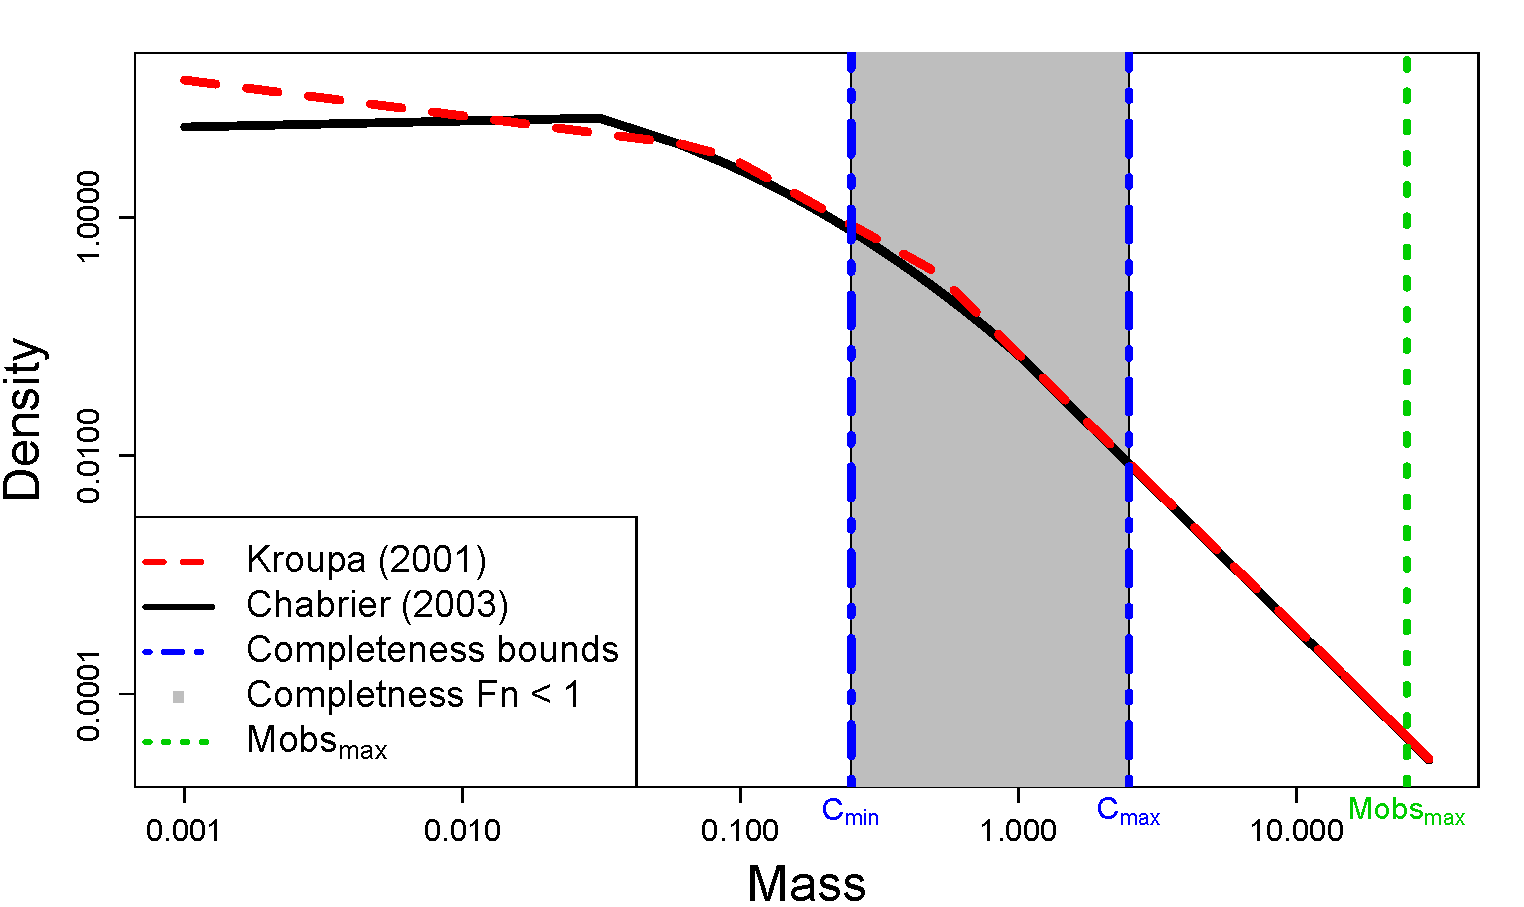
\includegraphics[width = .5\textwidth]{figures/CompareOthers3.pdf} 
   \caption{The broken power law model of \cite{kroupa2001} (red, dashed) and the lognormal with a power law tail model of \cite{Chabrier:2003om, Chabrier:2003oq} (black, solid) are displayed along with vertical lines representing several observational challenges.  The blue vertical dotted-dashed lines indicate the range of values ($C_{\min}, C_{\max}$) on which the completeness function may be defined, and the vertical green dotted line indicates the maximum observable mass (Mobs$_{\max}$) due to the aging cutoff.  The observational challenges are discussed further in \S\ref{sec:obs_challenges}.}
   \label{fig:imf_models}
\end{figure}


There are additional uncertainties involved in translating the actual observables  (e.g. photometric magnitudes) into a mass measurement; that is, the mass values for observable stars are only estimates. The {\it Hertzsprung-Russell (H-R) Diagram} is a classic visual summary of the distribution of the luminosity and temperature of a collection of stars. A typical H-R Diagram includes a {\it main sequence} of stars that trace a line from bright and hot stars to dim and cool stars. Stellar mass also evolves along this one-dimensional feature, and since luminosity and temperature are estimable, mass can thus also be estimated. The mass of binary stars can be determined via Kepler's Laws, and hence a {\it mass-luminosity relationship} can be fit to binaries and then extended to other stars on the main sequence. Unfortunately, luminosity and temperature are nontrivial to estimate, as corrections for effects such as {\it accretion} and {\it extinction} are required, along with an accurate estimate of the distance to the stars \citep{Da-Rio:2010aa}. 
The process is further complicated by the dependence of how these transformations are made on the {\it spectral type} of the star. Careful budgeting of the errors that accumulate is required in order to produce a reasonable error bars on mass estimates; \cite{Da-Rio:2010aa} utilize a Monte Carlo approach in which the errors in magnitudes are propagated forward through to uncertainties in the spectral type, the accretion and reddening corrections, and finally to an uncertainty on the mass.  


\subsection{Approximate Bayesian Computation}

Standard approaches to Bayesian inference, either analytical or built on
MCMC, require the specification of a
likelihood function, $f(m \mid \btheta)$, with data $\mobs \in \mathcal D$, 
and parameter(s) $\btheta \in \Theta$. In many modern scientific inference 
problems, such as for some emerging models for the stellar IMF, the likelihood is too complicated to be derived or otherwise
specified. 
As noted previously, ABC provides an approximation to the posterior
without specifying a likelihood function, and instead relies on forward simulation of the data generating
process.

The basic algorithm for sampling from the ABC posterior is attributed to 
\cite{TavareEtAl1997} and \cite{PitchardEtAl1999}, used for applications to population 
genetics. The algorithm has three main steps which are repeated until a sufficiently
large sample is generated:
\emph{Step 1}, Sample $\btheta^*$ from the prior; \emph{Step 2}, 
Generate $\msim$ from forward process assuming truth $\btheta^*$; 
 \emph{Step 3},  
Accept $\btheta^*$ if some distance function $\rho(\mobs, \msim) \leq \epsilon$, where $\epsilon$ is a tuning parameter that should be close to 0.
This last step typically consists of comparing low-dimensional summary statistics generated
for the observed and simulated datasets. 
Adequate statistical and computational performance of ABC algorithms depends greatly on the
selection of such summary statistics
\citep{JoyceMarjoram2008,BlumFrancois2010, Blum2010, FearnheadPrangle2012, BlumEtAl2013}.

The basic ABC algorithm can be inefficient in cases where the parameter space is of moderate
or high dimension.
Hence, important adaptations of the basic ABC algorithm incorporate ideas of sequential Monte Carlo (SMC) in 
order to improve the sampling efficiency \citep{MarjoramEtAl2003,SissonEtAl2007,beaumont2009, DelMoralEtAl2011}.  A nice overview of ABC can be found in \cite{MarinEtAl2012}.  
Here, we use a sequence of decreasing tolerances $\epsilon_{1:T} = (\epsilon_1, \ldots, \epsilon_T)$ 
with the tolerance $\epsilon_t$ shrinking until further reductions do not significantly affect the 
resulting ABC posterior.
The improvement in efficiency is due to the modification that happens after the first time step: 
instead of sampling from the prior distribution, the proposed $\btheta$ are drawn from the previous time step's ABC posterior.  Using this adaptive proposal distribution can help to improve the sampling efficiency.  The resulting draws, however, are not targeting the correct posterior, and so importance weights, $W_t$, are used to correct this discrepancy.

%----------------------------------------------------------------------------------------------------------------------------------------------
%-----------------------------------------------------------------------------------------------Methodology
%----------------------------------------------------------------------------------------------------------------------------------------------


\section{Forward Model for the IMF}
\label{PAmodelSection}
% Reason for doing this
Due to their simple interpretations, mathematical ease, and demonstrated consistency with observations, power law IMFs (or similar variants) have been widely adopted in the astronomy literature \citep{kroupa2012}; however, open questions remain about stellar formation processes.  The proposed forward model is a way to link a possible stellar formation process with the realized mass function (MF).  One known underlying mechanism for producing data with power-law tails is based on {\em preferential attachment} (PA).  
The earliest PA model, the Yule-Simon process, was popularized by \cite{simon55}, and was originally used to model biological genera and word frequencies\jessi{add more citations}.  \jessi{make connection to IMF}


\subsection{Preferential attachment for the IMF}

{\color{red} describe formation theory we are going to try to capture.}  
% Advantages 
%For physical interpretation, the model \eqref{eq:PAstars} has several advantages over the random sampling model of \cite{weisz13}. 
Rather than assuming that stellar masses in a cluster arise independently of each other, our PA model proposes a resource-limited mass accretion process between stellar cores whose ability to accumulate additional mass is a function of their existing masses. 
This dependence feature is particularly important for statistical inference, as models that assume independent observations of stellar masses are vulnerable to incorrect and misleading inference. 
Additionally, the mass of the largest star to form in a cluster is limited by the total cluster mass.


Our proposed stochastic model for stellar formation is as follows:~we first fix a total available cluster mass $\Mtot$. 
This quantity can be physically interpreted as the total mass available for stellar formation in a molecular cloud. 
At each time step $t = 1, 2, \ldots$, a random quantity of mass $m_t \sim Exponential(\lambda)$ enters the collection of stars; $M_{1,1} = m_1$ becomes the mass of the first star.
Subsequent masses entering the system form a new star with probability $\pi_t$ or join existing star $k = 1, \ldots, n_t$ with probability $\pi_{kt}$.
These probabilities are specified as
\begin{align}
	\pi_t = \min \left (1, \alpha \right ) \;\;\; \text{and} \;\;\; \pi_{kt} \propto M_{k,t}^{\gamma}\text{.}
\label{eq:PAstars}
\end{align}
The generating process is complete when the total mass of formed stars reaches $\Mtot$. 
The possible ranges of the three parameters are $\lambda > 0$, $\alpha \in [0,1)$, and $\gamma > 0$. 

% Interpretation
The parameter $\alpha$ defines the probability that entering mass forms a new star in a cluster.  For the growth component, the model allows for linear ($\gamma = 1$), sublinear ($\gamma < 1$), and superlinear ($\gamma > 1$) behavior; the limiting case of $\gamma \to 0$ gives a uniform attachment model.  Finally, the parameter $\lambda$ acts as a scaling factor which controls the average `coarseness' of masses joining the forming stellar cores. 

% We can get close to the usual IMF models 
The proposed PA mass generation model offers considerable flexibility to approximate existing IMF models in the literature.  To illustrate the generality of the proposed model, IMF realizations were drawn assuming the \cite{kroupa2001} 
%
broken power-law model as the true model, defined as
\begin{equation}
f(m) \propto \left\{
  \begin{array}{lr}
   m^{-0.3}, &  m \leq 0.08 \\
   k_1 \cdot m^{-1.3}, &  0.08 < m \leq 0.5 \\
   k_2 \cdot m^{-2.3}, &  m > 0.5,
  \end{array}
\right. \label{eq:kroupa}
\end{equation}
%
and the \cite{Chabrier:2003om, Chabrier:2003oq} lognormal model, defined as
%
\begin{equation}
f(m) \propto \left\{
  \begin{array}{lr}
    \frac{0.158}{m} \times \exp \left ( -\frac{(\log_{10}(m) - \log_{10}(0.079))^2}{2(0.69)^2}\right), &  m \leq 1\\
   k_3 \cdot m^{-2.3}, &  m > 1,
  \end{array}
\right. \label{eq:chab}
\end{equation}
%
where constants $k_1$, $k_2$, and $k_3$ are defined to make the densities continuous.
%
Our proposed PA ABC procedure was then used for inference and Figure~\ref{fig:otherModels} displays the resulting posterior predictive IMFs.  The proposed model captures the general shape of the true model.  Figures~\ref{subfig:kc_k} - \ref{subfig:kc_gamma} display ABC marginal posteriors for the broken power-law model of \cite{kroupa2001} and the lognormal model of  \cite{Chabrier:2003om, Chabrier:2003oq}.  Both the broken power-law and lognormal models have similar ABC posterior means for $\alpha$ (0.293 and 0.304, respectively).  However, the ABC posterior means for $\gamma$ are notably different.  The broken power-law model has an ABC posterior mean of 0.889 while the estimate for the lognormal model is 1.050.
\jessi{perhaps expand on the previous points to emphasize why this may be scientifically interesting}

\begin{figure} \centering
	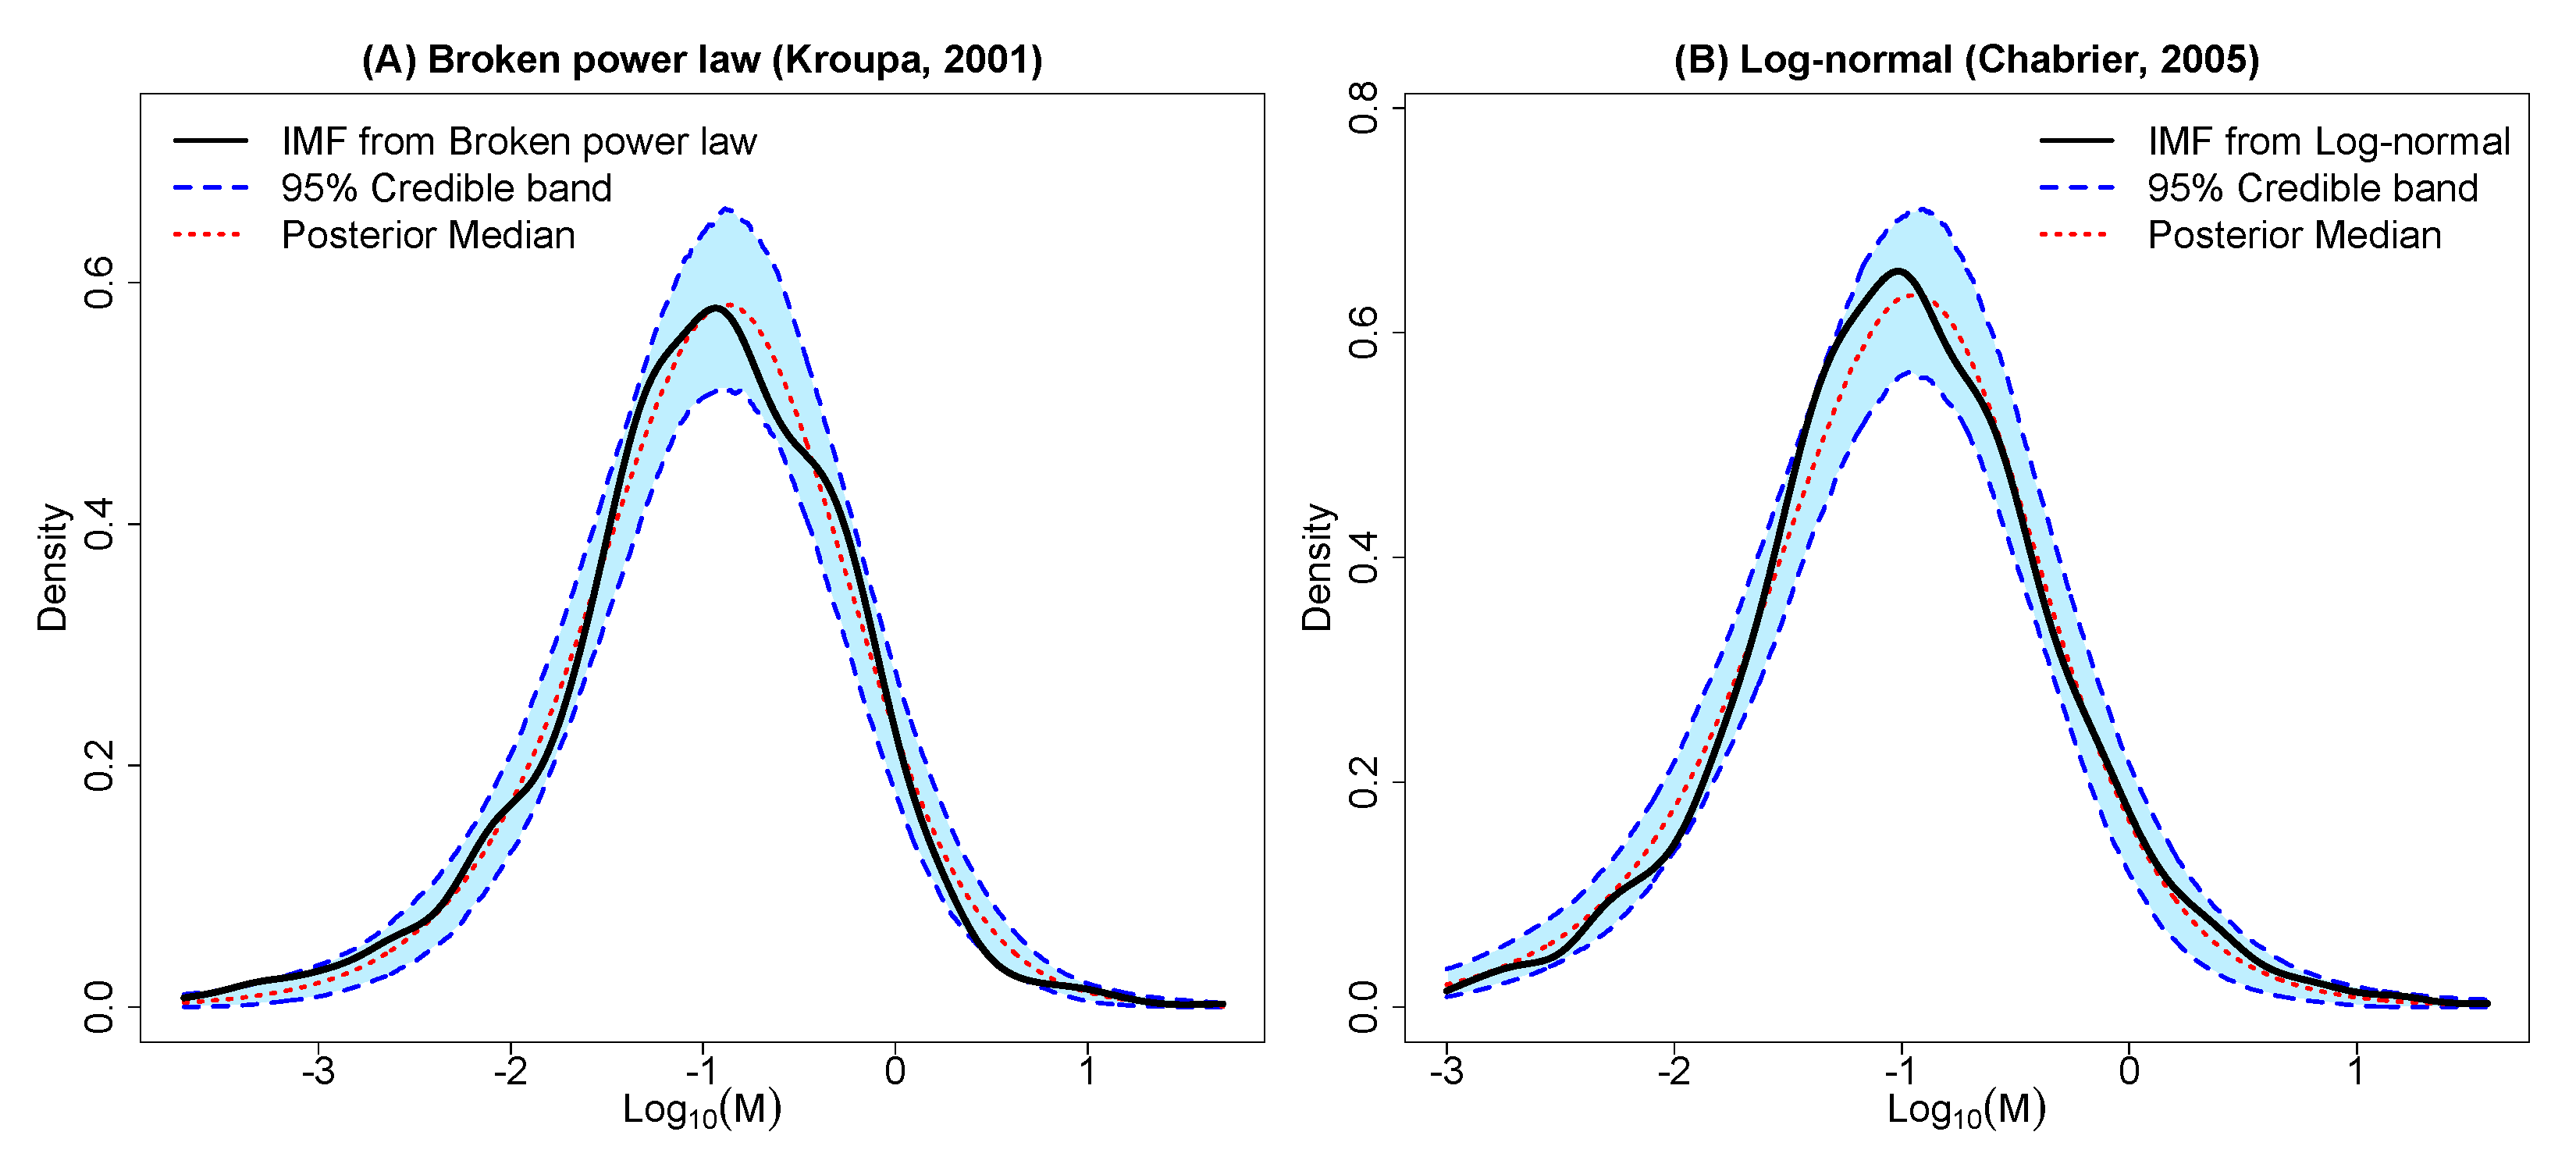
\includegraphics[width=0.85\textwidth]{figures/KroupaChabrier.pdf}
	\vspace{-0.1in}
	\caption{The solid black lines display the IMF with 1,000 stars simulated from (A) the broken power-law model of \cite{kroupa2001} (see Eq~\eqref{eq:kroupa}) and (B) the log-normal model of \cite{Chabrier:2003om, Chabrier:2003oq}  (see Eq~\eqref{eq:chab}).  The proposed PA ABC model was used with $N = 1,000$ particles, and 95\% point-wise credible bands are displayed (blue, dashed lines) along with the posterior median (red, dotted) for each data set.  The preferential attachment model provides flexibility to approximate both existing models.
Both models have similar ABC posterior means for $\alpha$ (0.293 and 0.304, respectively).  However, the ABC posterior means for $\gamma$ are notably different.  The broken power-law model has an ABC posterior mean of 0.889 while the estimate for the lognormal model is 1.050.
	}
	\label{fig:otherModels}
\end{figure}




\begin{figure}[htbp]
\begin{subfigure}{0.32\textwidth}
\centering
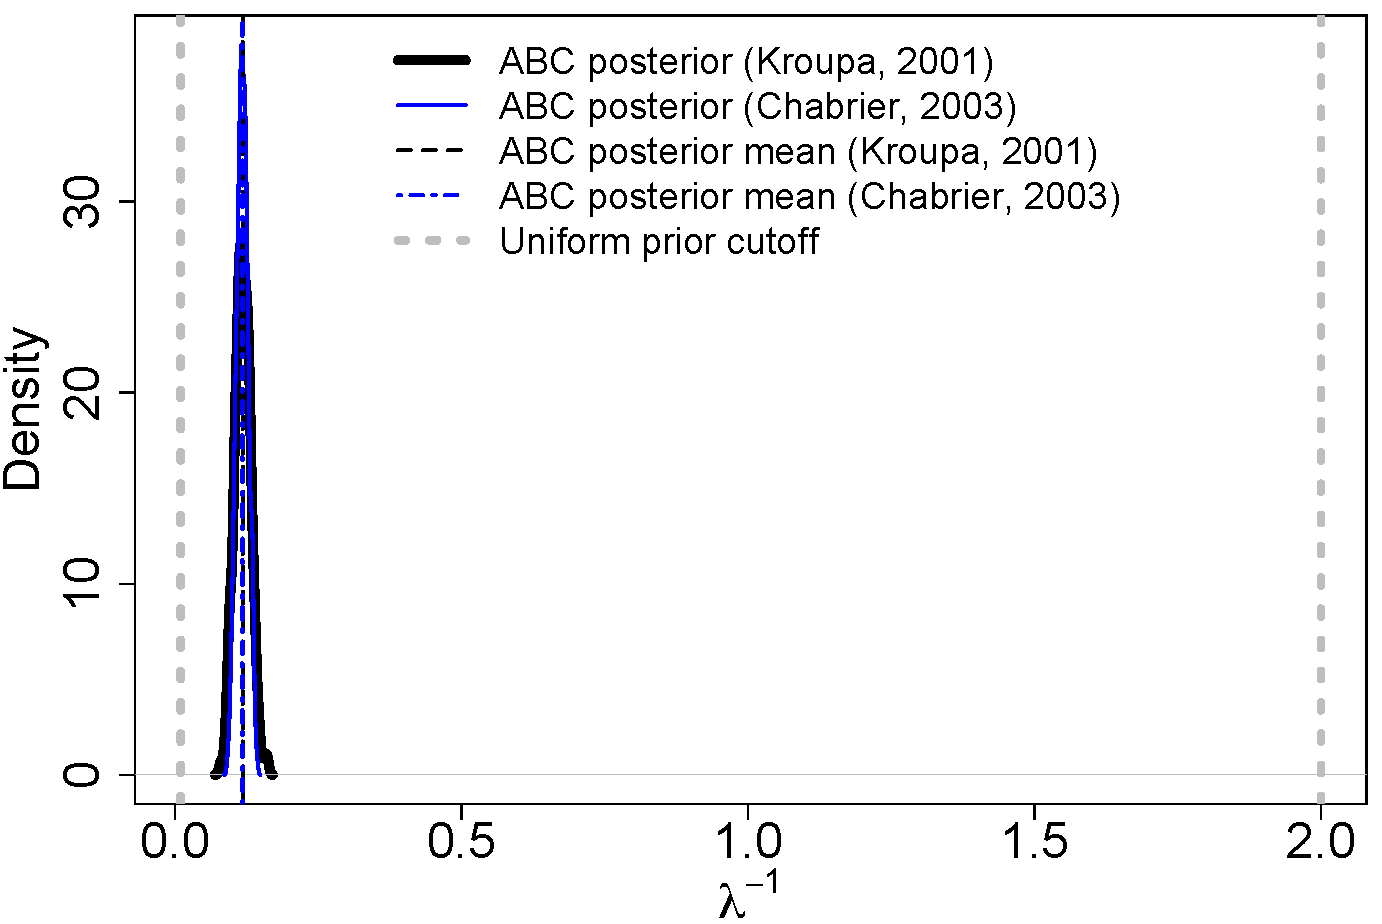
\includegraphics[width = .95\textwidth]{figures/kc_k.pdf} 
\caption{ABC posteriors for $\lambda^{-1}$}\label{subfig:kc_k}
\end{subfigure}
\begin{subfigure}{0.32\textwidth}
\centering
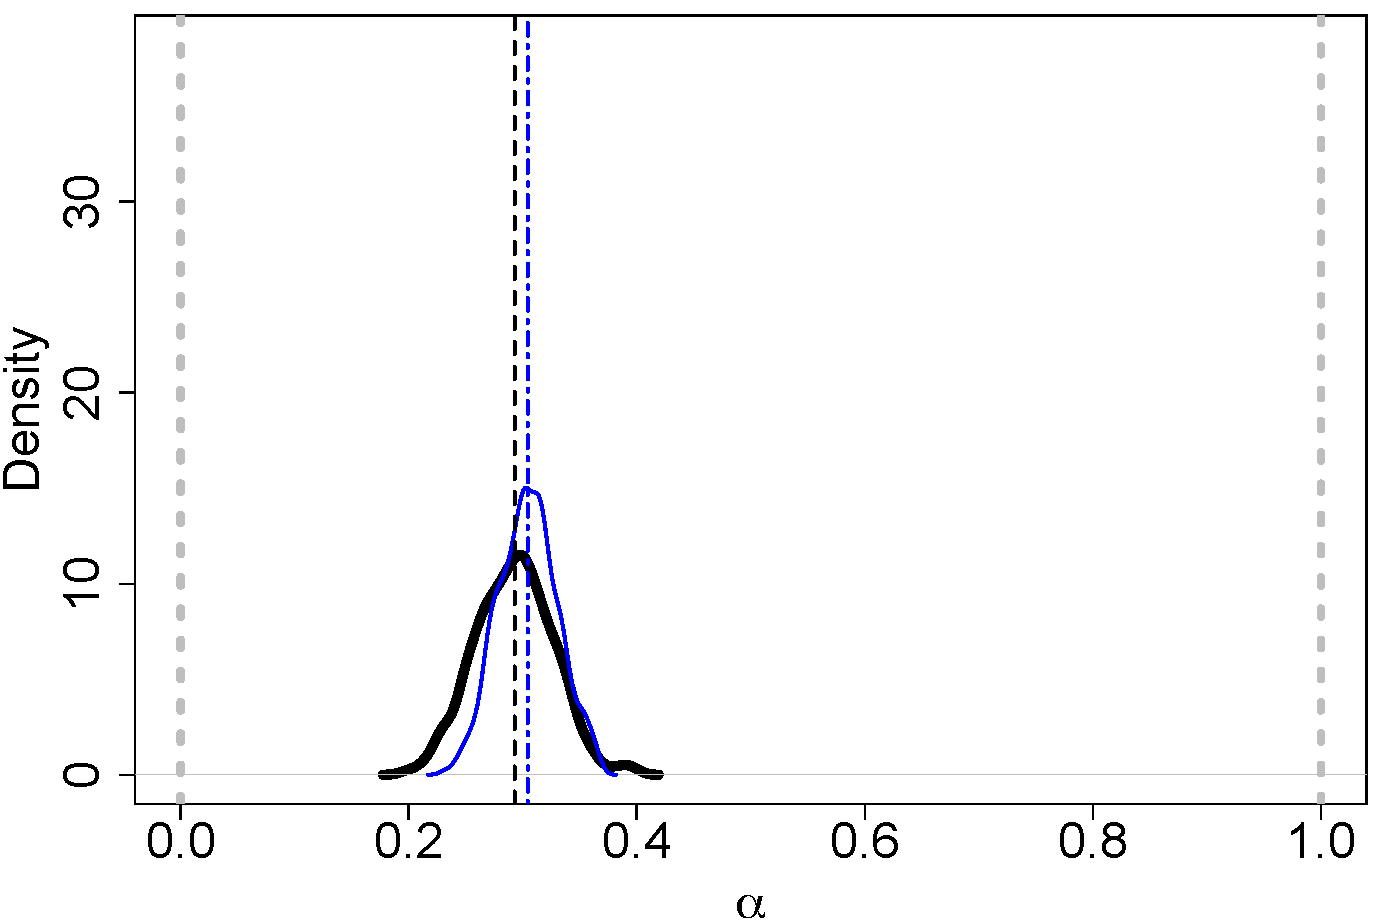
\includegraphics[width = .95\textwidth]{figures/kc_alpha.pdf} 
\caption{ABC posteriors for $\alpha$}\label{subfig:kc_alpha}
\end{subfigure}
\begin{subfigure}{0.32\textwidth}
\centering
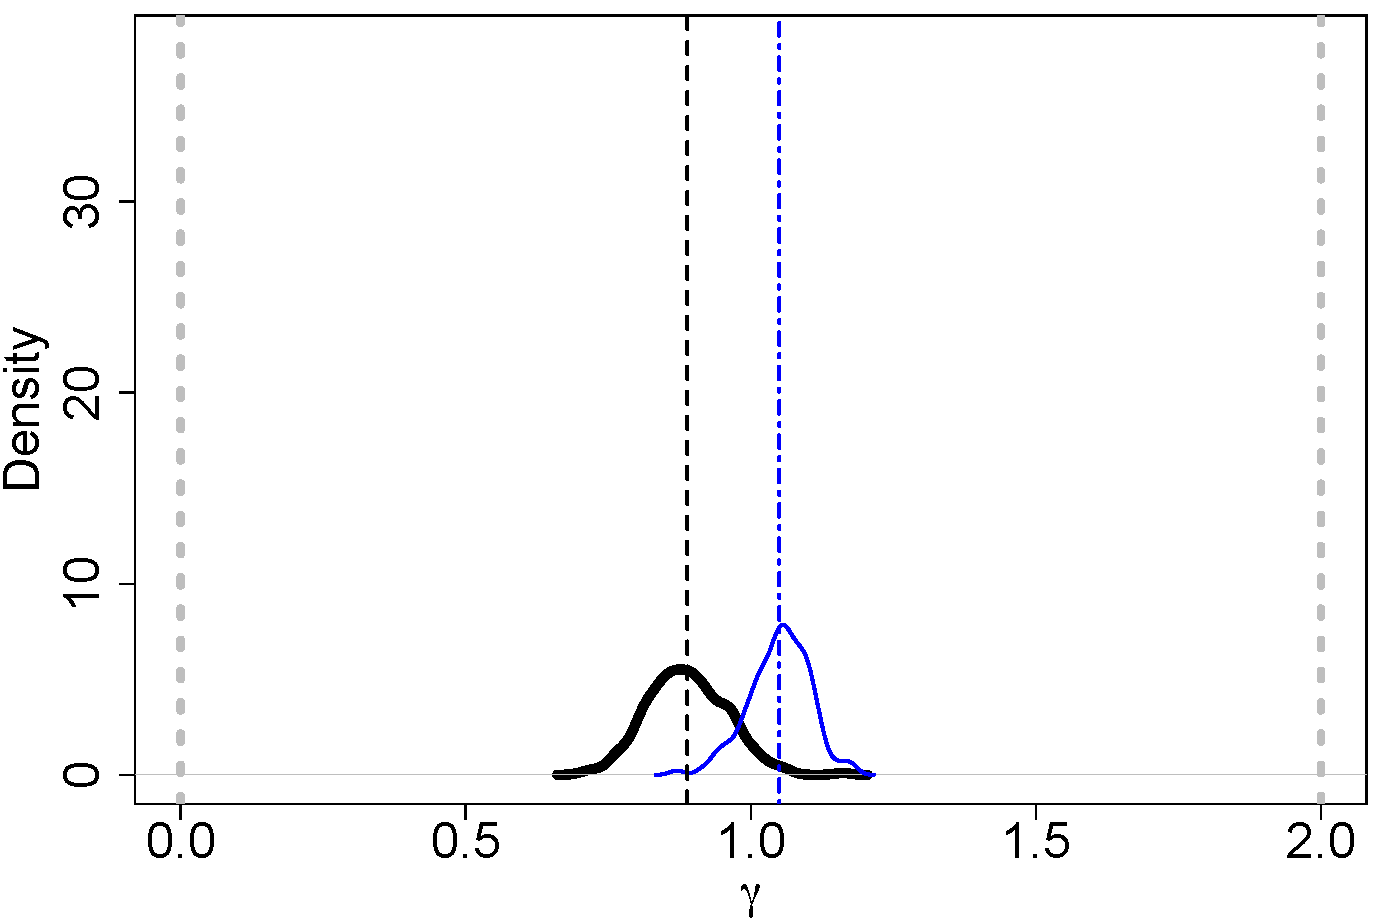
\includegraphics[width = .95\textwidth]{figures/kc_gamma.pdf} 
\caption{ABC posteriors for $\gamma$}\label{subfig:kc_gamma}
\end{subfigure} \\
%\begin{subfigure}{0.32\textwidth}
%\centering
%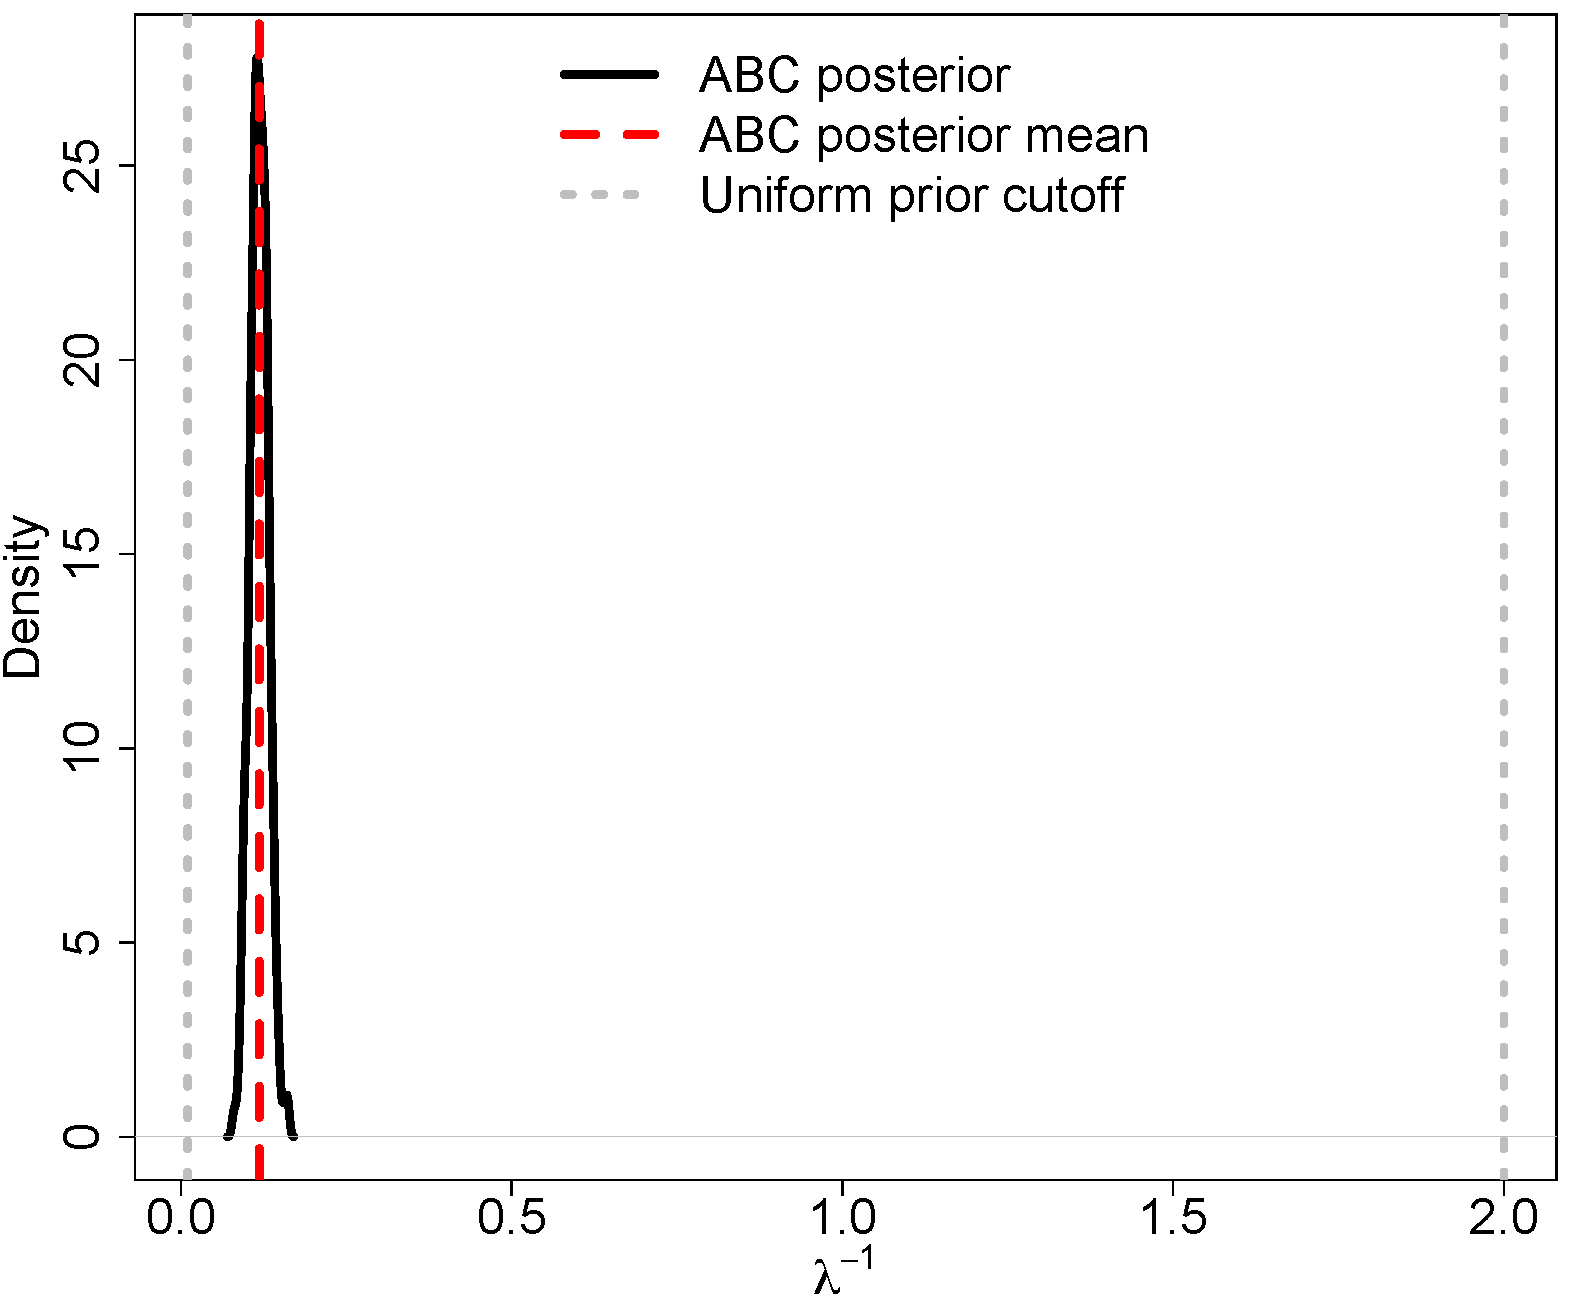
\includegraphics[width = .95\textwidth]{figures/kroupa_k.pdf} 
%\caption{ABC posterior for $\lambda^{-1}$}\label{subfig:kroupa_k}
%\end{subfigure}
%\begin{subfigure}{0.32\textwidth}
%\centering
%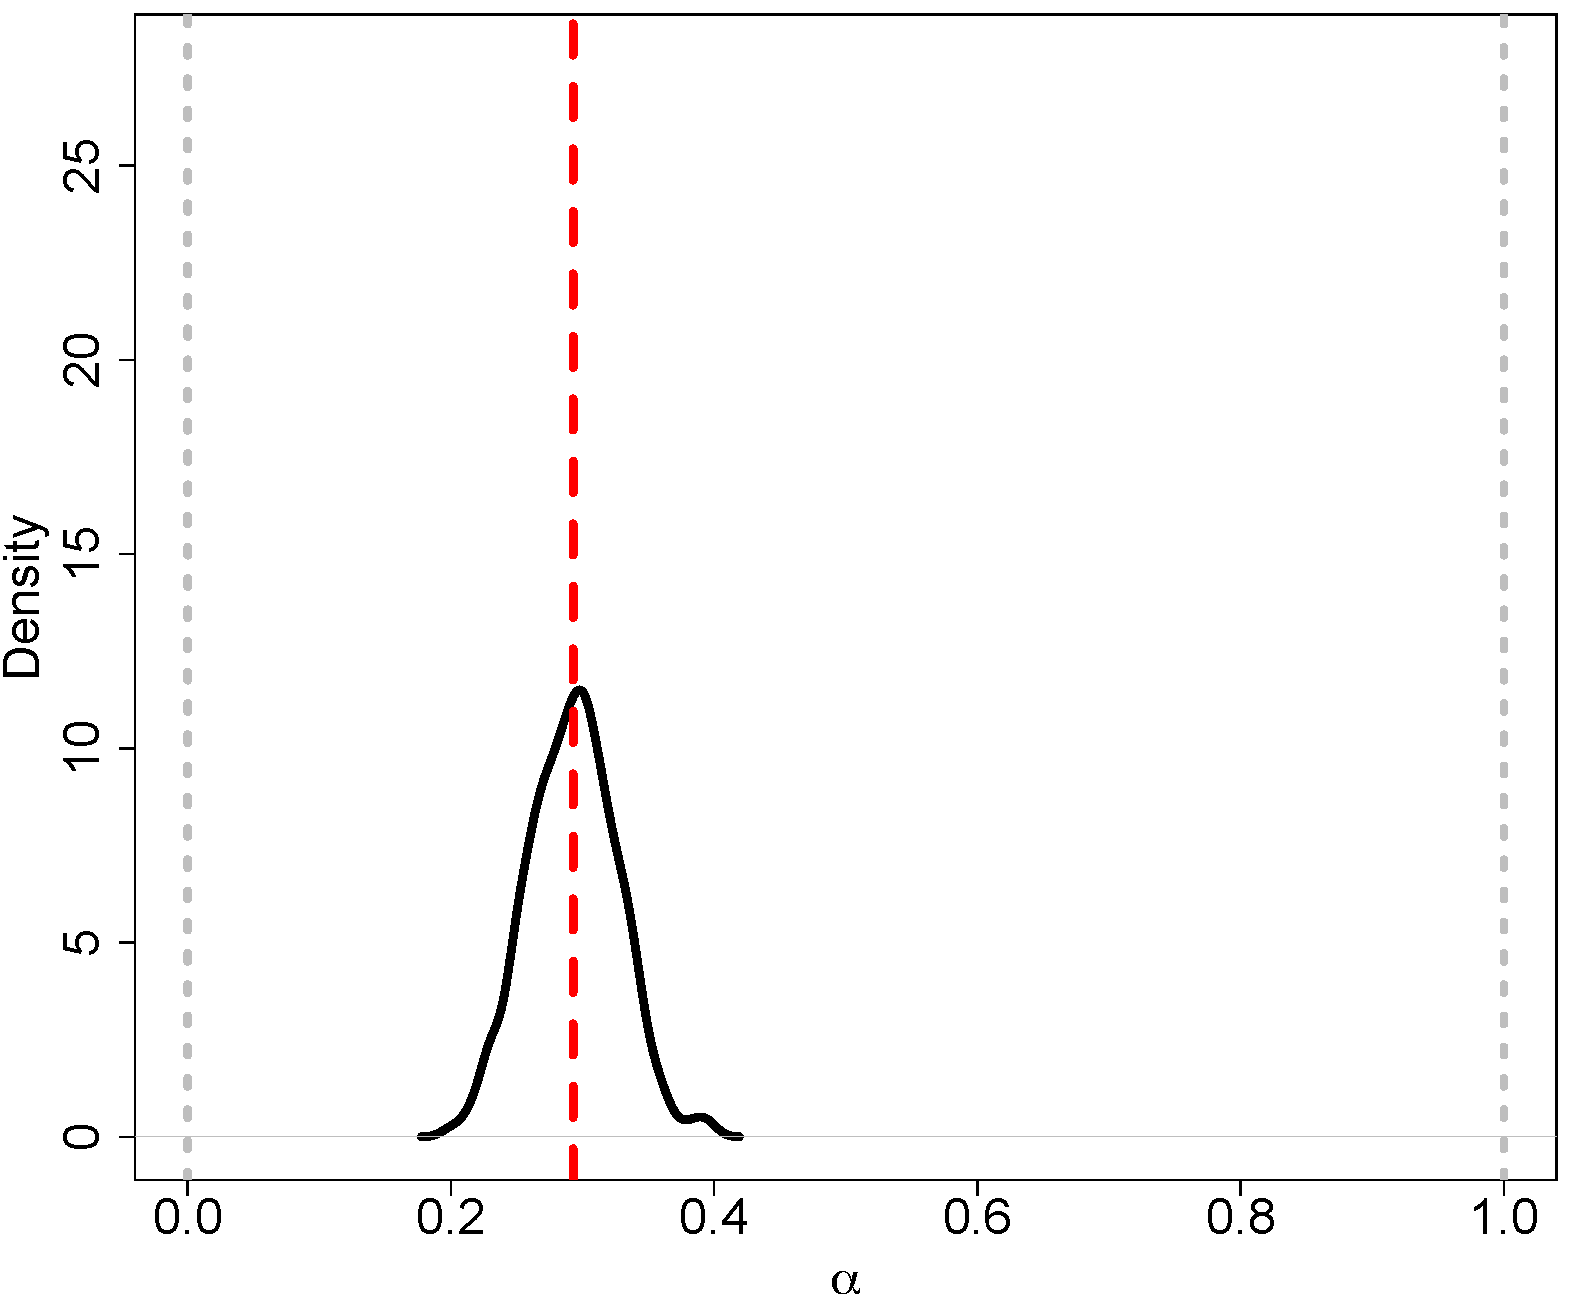
\includegraphics[width = .95\textwidth]{figures/kroupa_alpha.pdf} 
%\caption{ABC posterior for $\alpha$}\label{subfig:kroupa_alpha}
%\end{subfigure}
%\begin{subfigure}{0.32\textwidth}
%\centering
%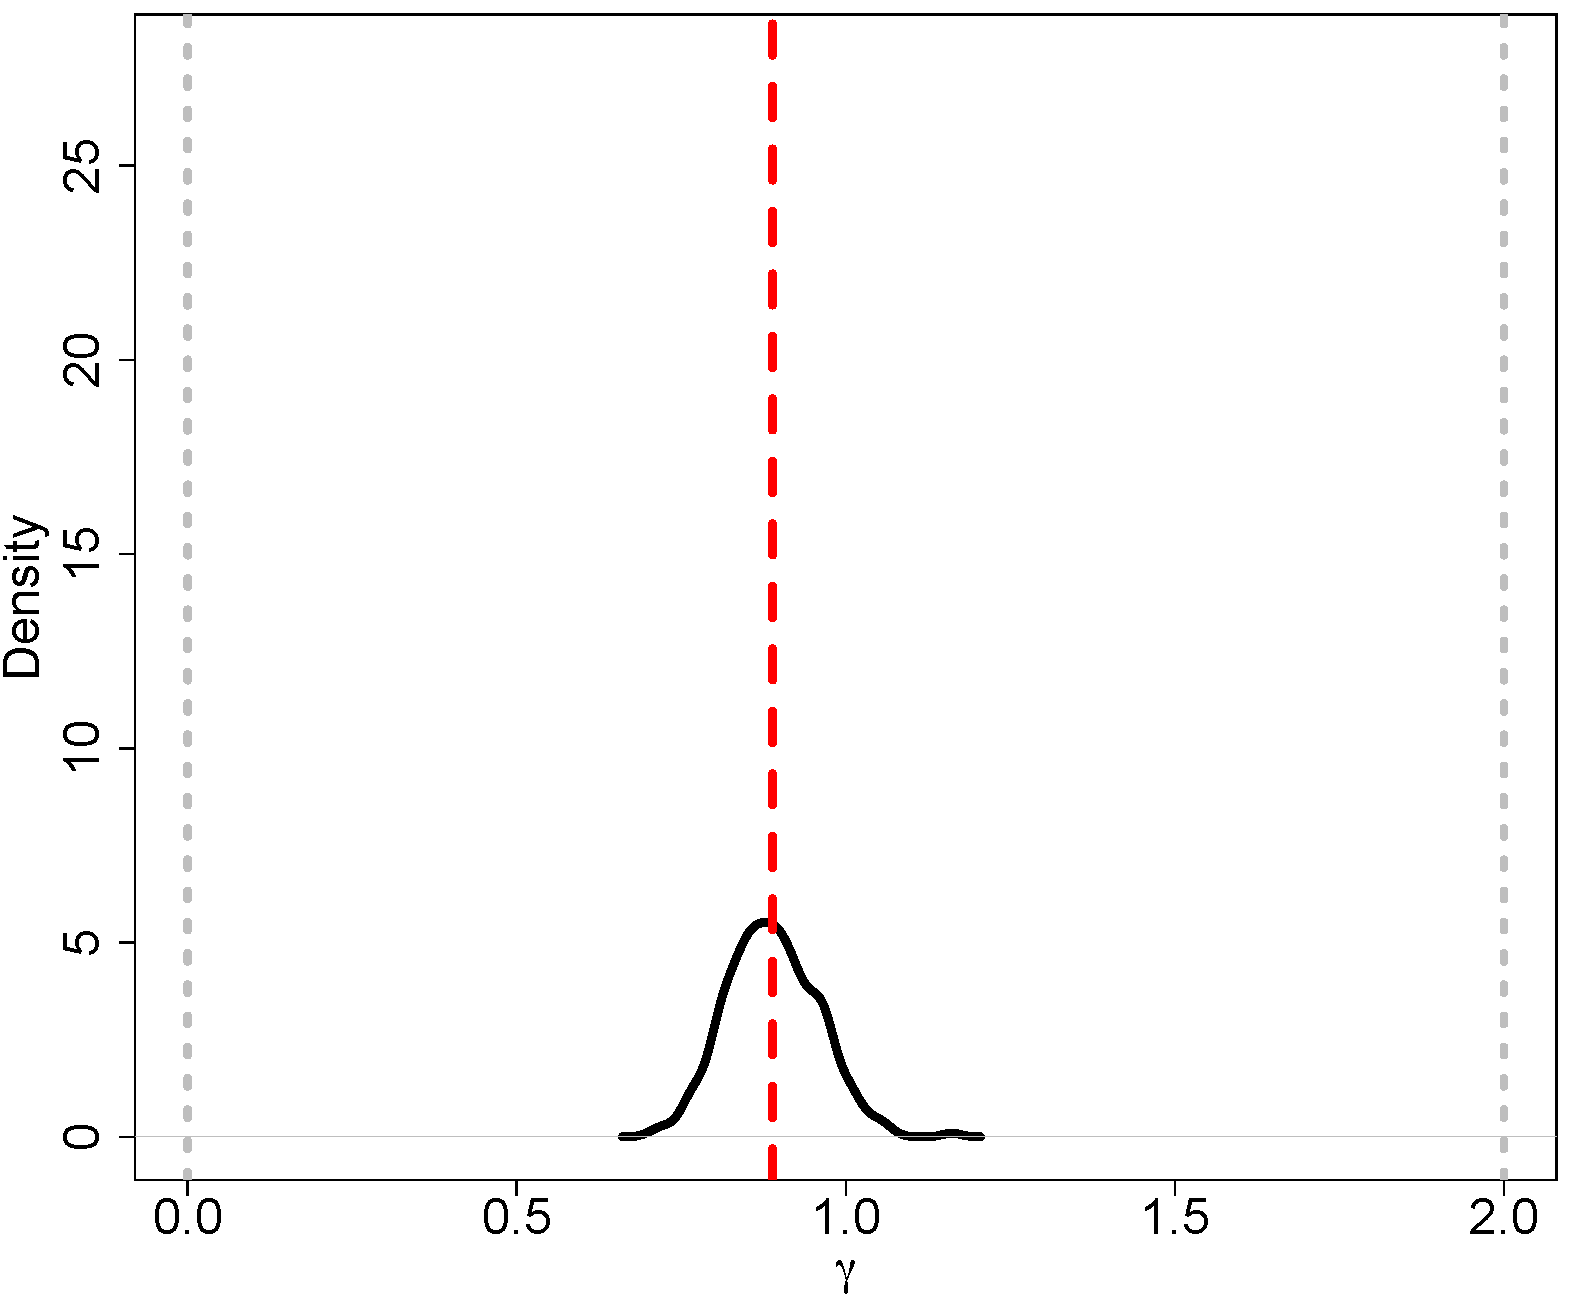
\includegraphics[width = .95\textwidth]{figures/kroupa_gamma.pdf} 
%\caption{ABC posterior for $\gamma$}\label{subfig:kroupa_gamma}
%\end{subfigure} \\
%\begin{subfigure}{0.32\textwidth}
%\centering
%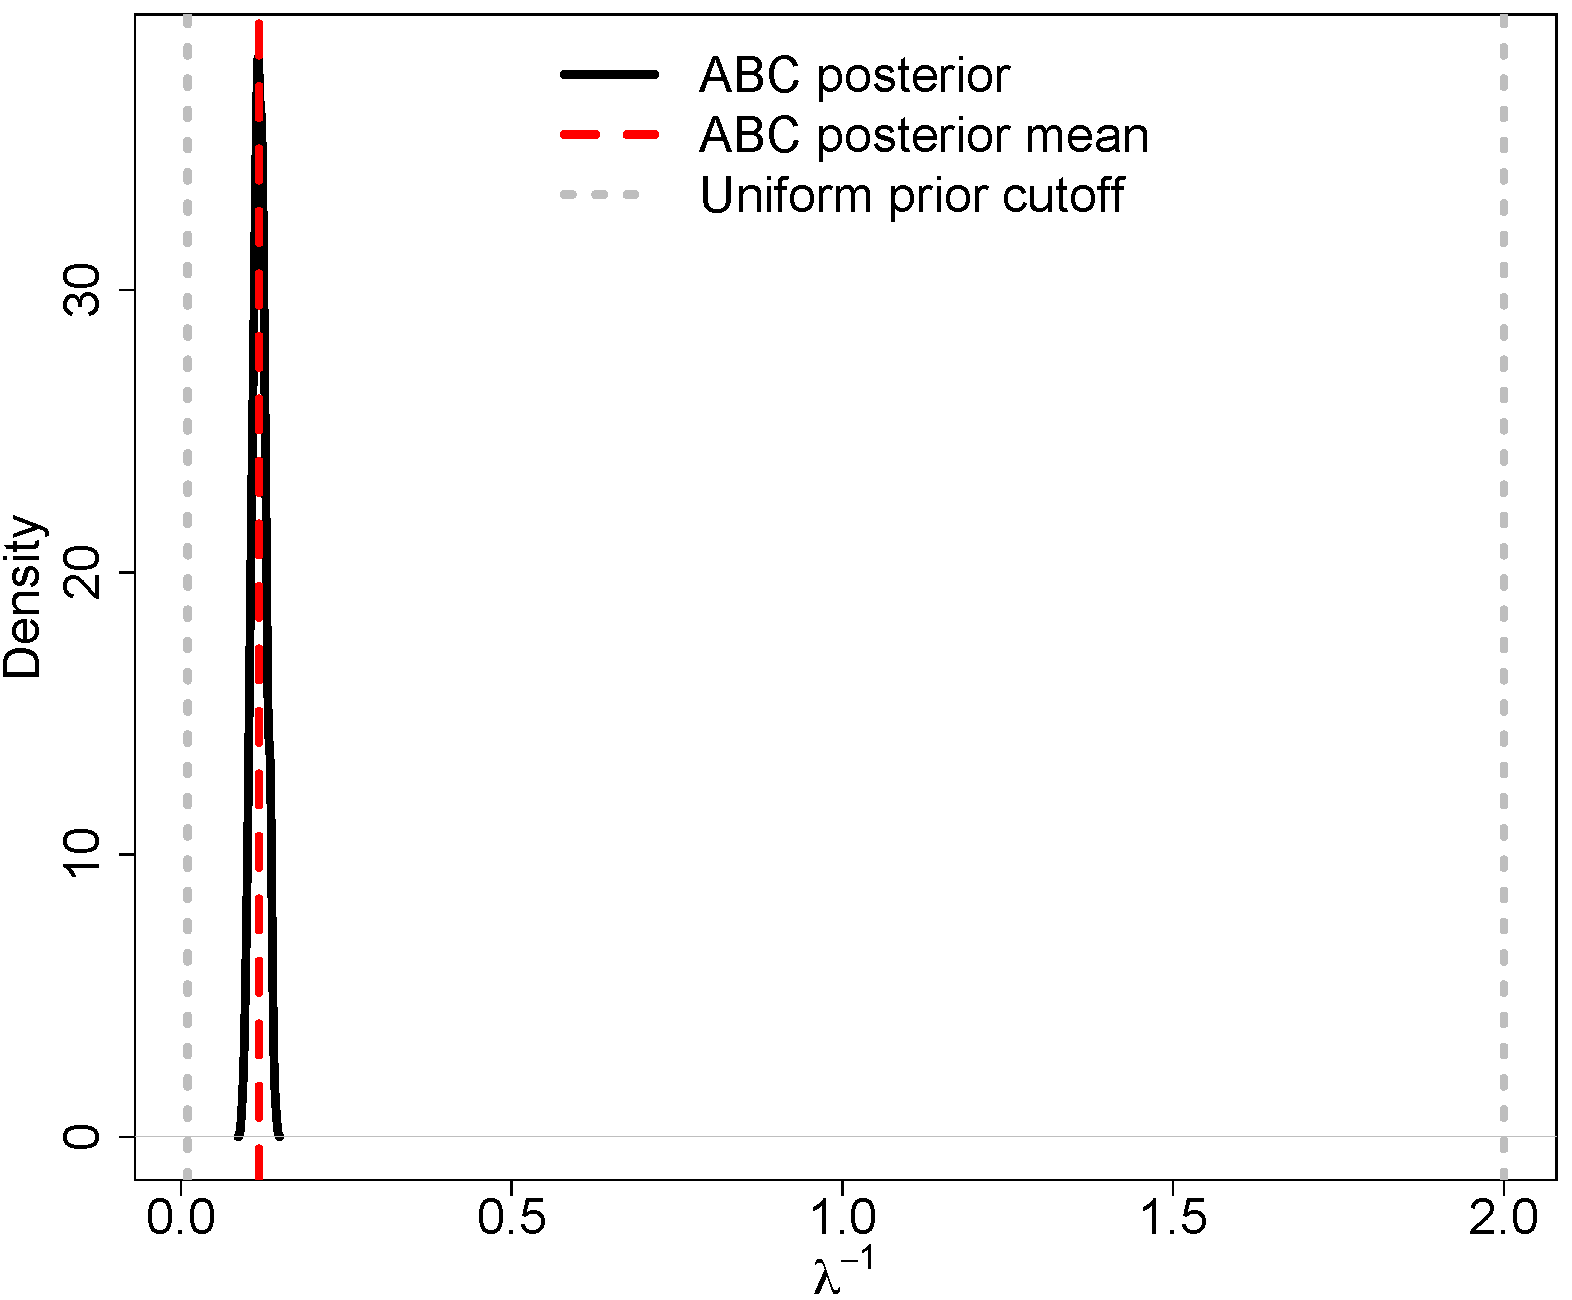
\includegraphics[width = .95\textwidth]{figures/chab_k.pdf} 
%\caption{ABC posterior for $\lambda^{-1}$}\label{subfig:chab_k}
%\end{subfigure}
%\begin{subfigure}{0.32\textwidth}
%\centering
%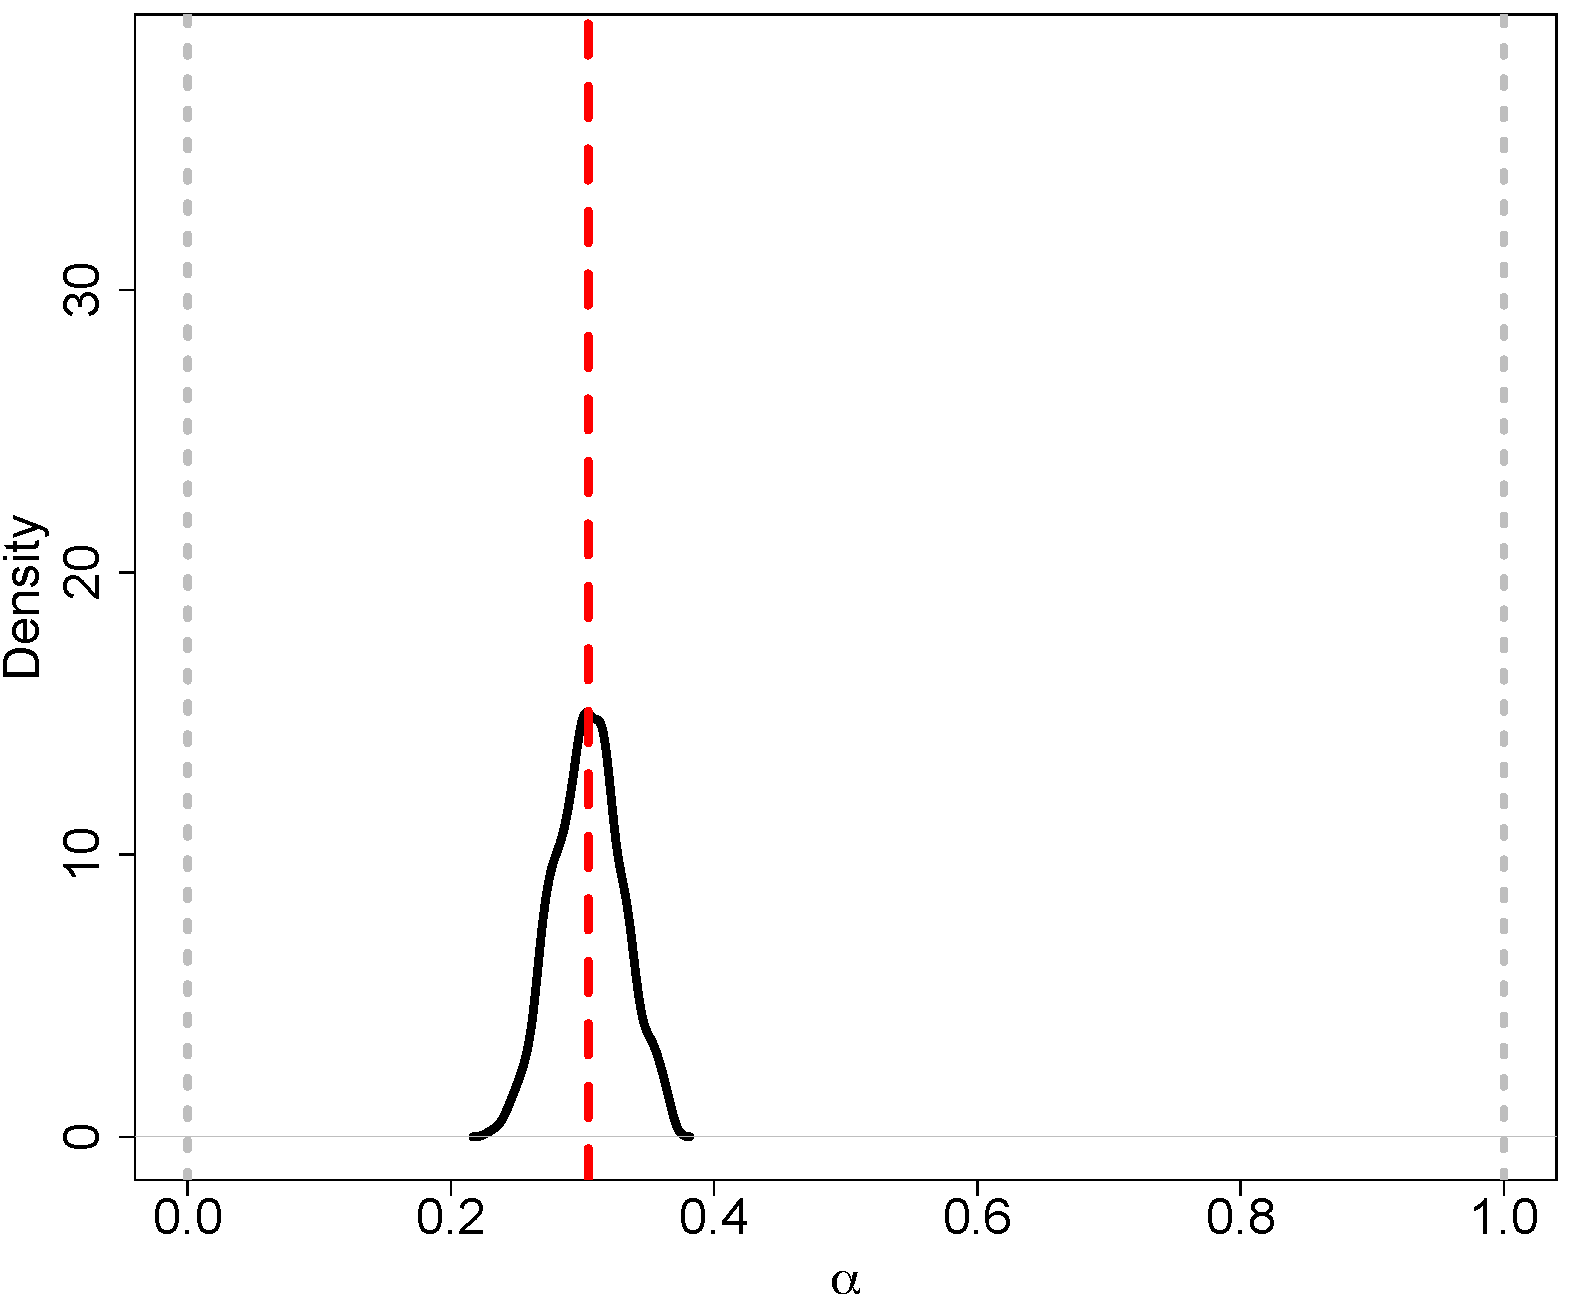
\includegraphics[width = .95\textwidth]{figures/chab_alpha.pdf} 
%\caption{ABC posterior for $\alpha$}\label{subfig:chab_alpha}
%\end{subfigure}
%\begin{subfigure}{0.32\textwidth}
%\centering
%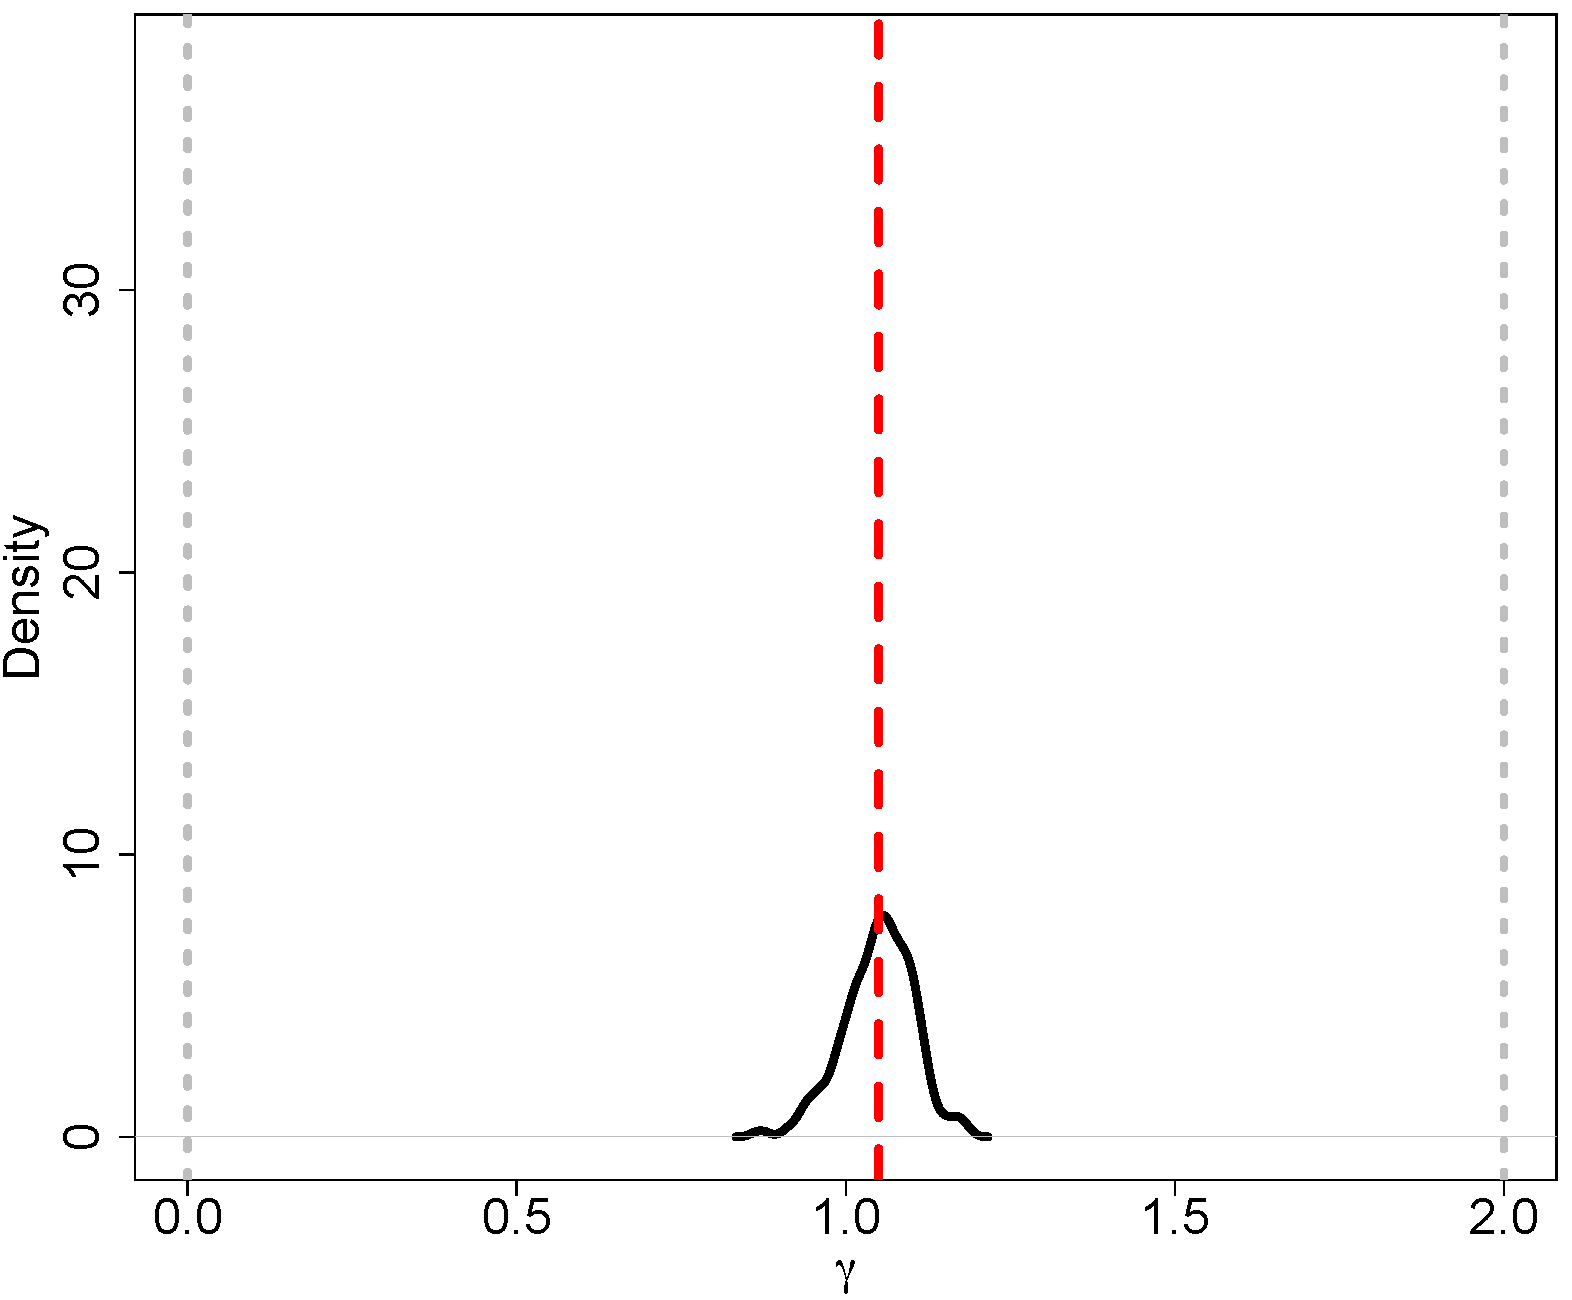
\includegraphics[width = .95\textwidth]{figures/chab_gamma.pdf} 
%\caption{ABC posterior for $\gamma$}\label{subfig:chab_gamma}
%\end{subfigure}
\caption{Marginal ABC posteriors for data generated from the broken power-law model of \cite{kroupa2001} (thick black lines)
and for data generated from the lognormal model of \cite{Chabrier:2003om, Chabrier:2003oq} (thin blue lines).  The vertical dashed black lines indicate the ABC posterior mean for the \cite{kroupa2001} model, vertical dashed and dotted blue lines indicate the ABC posterior mean for the \cite{Chabrier:2003om, Chabrier:2003oq} model, and the dotted gray lines indicate the range of the uniform prior for the parameter.  
 }
\label{fig:kroupa_chab_marginals}
\end{figure}




\subsubsection{Connection to power law tails?}
In the stellar formation context, linear PA models generate power law IMFs; sublinear variants produce slight deviations from power laws, 
and exponential cutoffs can also be induced. \jessi{I'm not sure about the previous statement - it may have been written in a much earlier draft.  It can/should be revised based on what we decide to include in the discussion about the power law tails}




\subsection{Initial Mass Function to the Observed Mass Function} \label{sec:obs_challenges}
The PA model describes the formation of a star cluster at initial formation.  However, we are not generally able to observe the star cluster after initial formation due to observational uncertainties, measurement uncertainties, and aging and dynamical evolution of the cluster.  A cluster's present-day observed mass function (MF) is the observed distribution of the stellar masses of a particular cluster.

% Completeness functions
Observation limitations can be easily incorporated into the ABC framework.  For simplicity, we adopt a ``linear ramp" completeness function describing the probability of observing a star of mass $m$:
\begin{align}
	\Proba(\text{observing a star} \mid m) = \begin{cases} 0 \text{,} & m < \Cmin\\
								\frac{m - \Cmin}{\Cmax - \Cmin}\text{,} & m \in [\Cmin, \Cmax] \\
								1 \text{,} & m > \Cmax \text{.}
								\end{cases} \label{eq:ramp}
\end{align}
We assume that the values $\Cmin$ and $\Cmax$ are known, though we note that selecting an appropriate completeness function is a difficult process which requires quantification from the observational astronomers for each set of data.
Different models for the completeness function could also be considered, including those which allow for spatially-varying observational completeness.  A benefit of ABC is the ease at which a new completeness function can be incorporated -- it amounts to a simple change in the forward model.  

% Observational uncertainties - normal on log scale
Due to measurement error and practical limitations in translating luminosities into masses, the masses of stars are not perfectly known. 
This uncertainty can be incorporated in different ways; following \cite{weisz13}, we assume that the inferred mass of a star $m_i$ is related to its true mass $M_i$ via 
\begin{align}
	\log m_i = \log M_i + \sigma_i \eta_i \text{,}
	\label{eq:masserror}
\end{align}
where $\eta_i$ is a standard normal random variable, and $\sigma_i$ is known measurement error.   %Hence, the $m_i$ arise from a truncated IMF convolved with log-normal mass uncertainties.  
% Potential extensions
The model for mass uncertainties in \eqref{eq:masserror} is simple and could be extended to account for other sources of uncertainty (e.g. redshift).

% STELLAR EVOLUTION
As noted previously, the lifecycle of a star depends on certain characteristics such as mass.  In the proposed algorithm, stars generated in a cluster are aged using a simple truncation of the largest masses.  
That is, the distribution of stellar masses for a star cluster of age $\tau$ Myr is given by
	\begin{align}
	f_M(m \mid \theta, \tau) = f_M(m \mid \theta) \indic \{M \leq \tau^{-1/3} \times 10^{4/3}\} \text{,}
	\label{eq:age}
	\end{align}
corresponding to stellar lifetimes of 10$^4$ $M^{-3}$ Myr, where $M$ is the mass of the star \citep{hansen2004, Chaisson:2011}. 
More sophisticated models that account for effects such as binary stars and stellar wind mass loss can be inserted into this framework.  
%For example, \cite{schneider2014} proposes a stellar evolution model that accounts for the effects of binary stars, stellar wind mass loss, and other phenomena which impact the shape of the observed MF and have implications for inference on the most massive star that could initially form in a cluster.



\section{Methods}
\label{methodSec}

We propose an ABC framework to make inferences on the IMF given a cluster's present-day observed MF.  The proposed ABC algorithm is displayed in Algorithm~\eqref{alg1}, where $N$ is the desired particle sample size to approximate the posterior distribution, and is motivated by the adaptive ABC algorithm of \cite{beaumont2009}.  The forward model, $F$, in Algorithm~\eqref{alg1} is where observational limitations and uncertainties, stellar evolution, and other astrophysical elements can be incorporated as outlined in Section~\ref{PAmodelSection}.


\subsection{Proposed ABC algorithm}
Algorithm~\eqref{alg1} is initialized using the basic ABC rejection algorithm at time step $t = 1$ using a distance function $\rho(\msim, \mobs)$ to measure the distance between the simulated and observed datasets, $\msim$ and $\mobs$, respectively.  The first tolerance, $\epsilon_1$, is adaptively selected by drawing $kN$ particles for some $k >0$.  Then the $N$ particles that have the smallest distance are retained, and $\epsilon_1$ is defined as the largest of those $N$ distances retained.
%
For subsequent time steps ($t > 1$), rather than proposing a draw, $\theta^*$, from the prior, $\pi(\theta)$, the proposed $\theta^*$ is selected from the previous time step's ($t-1$) ABC posterior samples.  The selected $\theta^*$ is then moved according to some kernel, $K(\theta^*, \cdot)$, to ameliorate degeneracy as the sampler evolves.  In order to ensure the true posterior (which requires sampling from the prior) is targeted, the retained draws are weighted according to the appropriate importance weights, $W_t$ -- this incorporates the proposal distribution's kernel.


\begin{algorithm}[ht]
 \caption{Stellar IMF ABC algorithm with sequential sampling} \label{alg1}
 \KwData{Observed stellar masses, ($\mobs$)}
 \KwResult{ABC posterior sample of $\theta$}

 {\em At iteration $t = 1$:}\\
  \For{$j = 1, \ldots, kN$}{
% \While{$\rho(\msim, \mobs) > \epsilon_t$}{
 Propose $\theta_t^{(j)}$ by drawing $\theta_t^* \sim \pi(\theta)$ \\
 Generate cluster stellar masses $\msim$ from $F(m \mid \theta_t^*)$ \\
Calculate distance $\rho_t^{(j)} \gets \rho(\msim, \mobs)$
% }
 }
 
$\theta_t^{(j)} \gets \theta_t^{(l)}, l = $ index of $N$ smallest $\rho_t^{(q)}, q = 1, \ldots, kN$\\
$W_t^{(j)} \gets 1/N, j = 1, \ldots, N$\\

{\em At iterations $t = 2, \ldots, T$:}\\
 \For{$j = 1, \ldots, N$}{
 \While{$\rho(\msim, \mobs) > \epsilon_t$}{
 Select $\theta^{(j)}$ by drawing from the $\theta^{(i)}_{t-1}$ with probabilities $W^{(i)}_{t-1}, i = 1, \ldots, N$ \\
 Generate $\theta^{*(j)}$ from transition kernel $K(\theta^{(j)}, \cdot)$ \\
 Generate cluster stellar masses $\msim$ from $F(m \mid \theta^{*(j)})$ \\
% Calculate distance $\rho(\msim, \mobs)$
 }
$\theta_t^{(j)} \gets \theta^{*(j)}$\\
$W_t^{(j)} \gets \frac{\pi(\theta_t^{(j)})}{\sum_{i = 1}^N  W_{t-1}^{(i)} K(\theta_{t-1}^{(i)}, \theta_t^{(j)})} $
}
$W_t^{(j)} \gets \frac{W_t^{(j)}}{\sum_{l = 1}^N W_t^{(l)}}, j = 1, \ldots, N$ \bigskip
\end{algorithm}


A key step in the implementation of an ABC algorithm is to quantify the distance between the simulated and observed stellar masses.  We define a bivariate summary statistic and distance function that captures the shape of the present-day MF and the random number of stars observed, displayed in Equations~\eqref{eq:2da} and \eqref{eq:2db}, respectively.  For the shape of the present-day MF, we use a kernel density estimate of the $\log_{10}$ masses (due to the heavy-tailed distribution of the initial masses), and an $L_2$ distance between the simulated and observed $\log_{10}$ mass function estimates.  The number of stars observed is the other summary statistic, with the distance being the absolute value of the difference in the ratio of the counts from 1. The bivariate summary statistic is defined as
\begin{align}
\rho_1(\msim, \mobs) &= \left [\displaystyle \int \left \{\hat f_{\log \msim}(x) - \hat f_{\log \mobs}(x) \right \}^2 dx \right]^{1/2} \label{eq:2da} \\ 
\rho_2(\msim, \mobs) &= \max\left\{\left|1 - \nsim/ \nobs\right |, \left|1 - \nobs/ \nsim\right |  \right\} \text{,}   \label{eq:2db}
\end{align}
where the $\hat f$ are kernel density estimates, and $\nsim$ and $\nobs$ are the number of stars comprising the observed MF.  These summary statistics were selected based on performance of a simulation study using the high-mass section of the broken power-law model because the true posterior is known in this setting.  Results and additional discussion of the simulation study can be found in Appendix~\ref{app:summary}.

With the bivariate summary statistic, we use a bivariate tolerance sequence, $(\epsilon_{1t}, \epsilon_{2t})$, for $t = 1, \ldots, T$ is such that $\epsilon_{i1} \geq \epsilon_{i2} \geq \cdots \geq \epsilon_{iT}$ for $i = 1, 2$.  At time step $t$, the tolerances are determined based on the  empirical distribution of the retained distances from time step $t-1$ (e.g. the $25th$ percentile).  As noted previously, the tolerance sequence is initialized adaptively by selecting $kN$ proposals from the prior distributions, then the $N$ proposals that result in the $N$ smallest distances were selected.\footnote{The $kN$ sampled distances were scaled, squared, and then added together; the $N$ smallest of these combined distances were retained.}

In practice, $\Mtot$ is an unknown quantity of interest.  A prior can be assigned to $\Mtot$ and an additional summary statistic and tolerance sequence can be used.  The summary statistics we select in this case is
\begin{equation}
\rho_3(\msim, \mobs) = \left| \sum_{i = 1}^{\nsim} m_{\text{sim}, i} - \sum_{j = 1}^{\nobs} m_{\text{obs}, j} \right|, \label{eq:2dc}
\end{equation}
where $m_{\text{sim}, i}$ and $m_{\text{obs}, j}$ are the masses of the individual simulated and observed stars, respectively.  



\subsection{Simulation study}
A short simulation study was carried out to illustrate the performance of the proposed model in the case where the solution is known, using the summary statistics in Equations~\eqref{eq:2da}-\eqref{eq:2dc}.  Values for the parameters $(\lambda^{-1}, \alpha, \gamma, \Mtot)$ are displayed in Table~\ref{tab:sim_study} along with the number of stars produced, $\nobs$, which are used in the simulation as the observations.  The generated IMF's used as the observations for each setting are displayed in Figure~\ref{fig:true_imf}; number counts rather than densities are displayed in order to emphasize the different number of stars produced under each setting.


One of the more notable differences in the simulated IMFs displayed in Figure~\ref{fig:true_imf} used as the observations in the simulation study is the number of stars generated.  The $\alpha$ parameter controls the numbers stars that form and so there appears to be two groups of IMFs:  one with $\alpha = 0.3$ and one with $\alpha = 0.7$.  


\begin{table}[htbp]
\begin{minipage}[b]{0.48\linewidth}
\centering
   \begin{tabular}{|c|c|c|c|c|} % Column formatting, @{} suppresses leading/trailing space
   \hline
   Number & $\lambda^{-1}$ & $\alpha$ & $\gamma$  & $\Mtot$ \\
   \hline
1	&	0.25	&	0.3	&	0.5	& 1000 \\
2	&	0.25	&	0.3	&	1.0	& 1000 \\
3	&	0.25	&	0.3	&	1.5	& 1000 \\
4	&	0.25	&	0.7	&	0.5	& 1000 \\
5	&	0.25	&	0.7	&	1.0	& 1000 \\
6	&	0.25	&	0.7	&	1.5	& 1000 \\
\hline
   \end{tabular}
   \begin{tabular}{|c|} % Column formatting, @{} suppresses leading/trailing space
   \hline
 $\nobs$ \\
   \hline
1166	 \\
1142	 \\
1148	 \\
2801	 \\
2698	 \\
2710	 \\
\hline
   \end{tabular}
   \caption{Parameter values for the simulation study and the number of stars in the data set, $\nobs$.}
   \label{tab:sim_study}
\end{minipage}\hfill
\begin{minipage}[b]{0.48\linewidth}
\centering
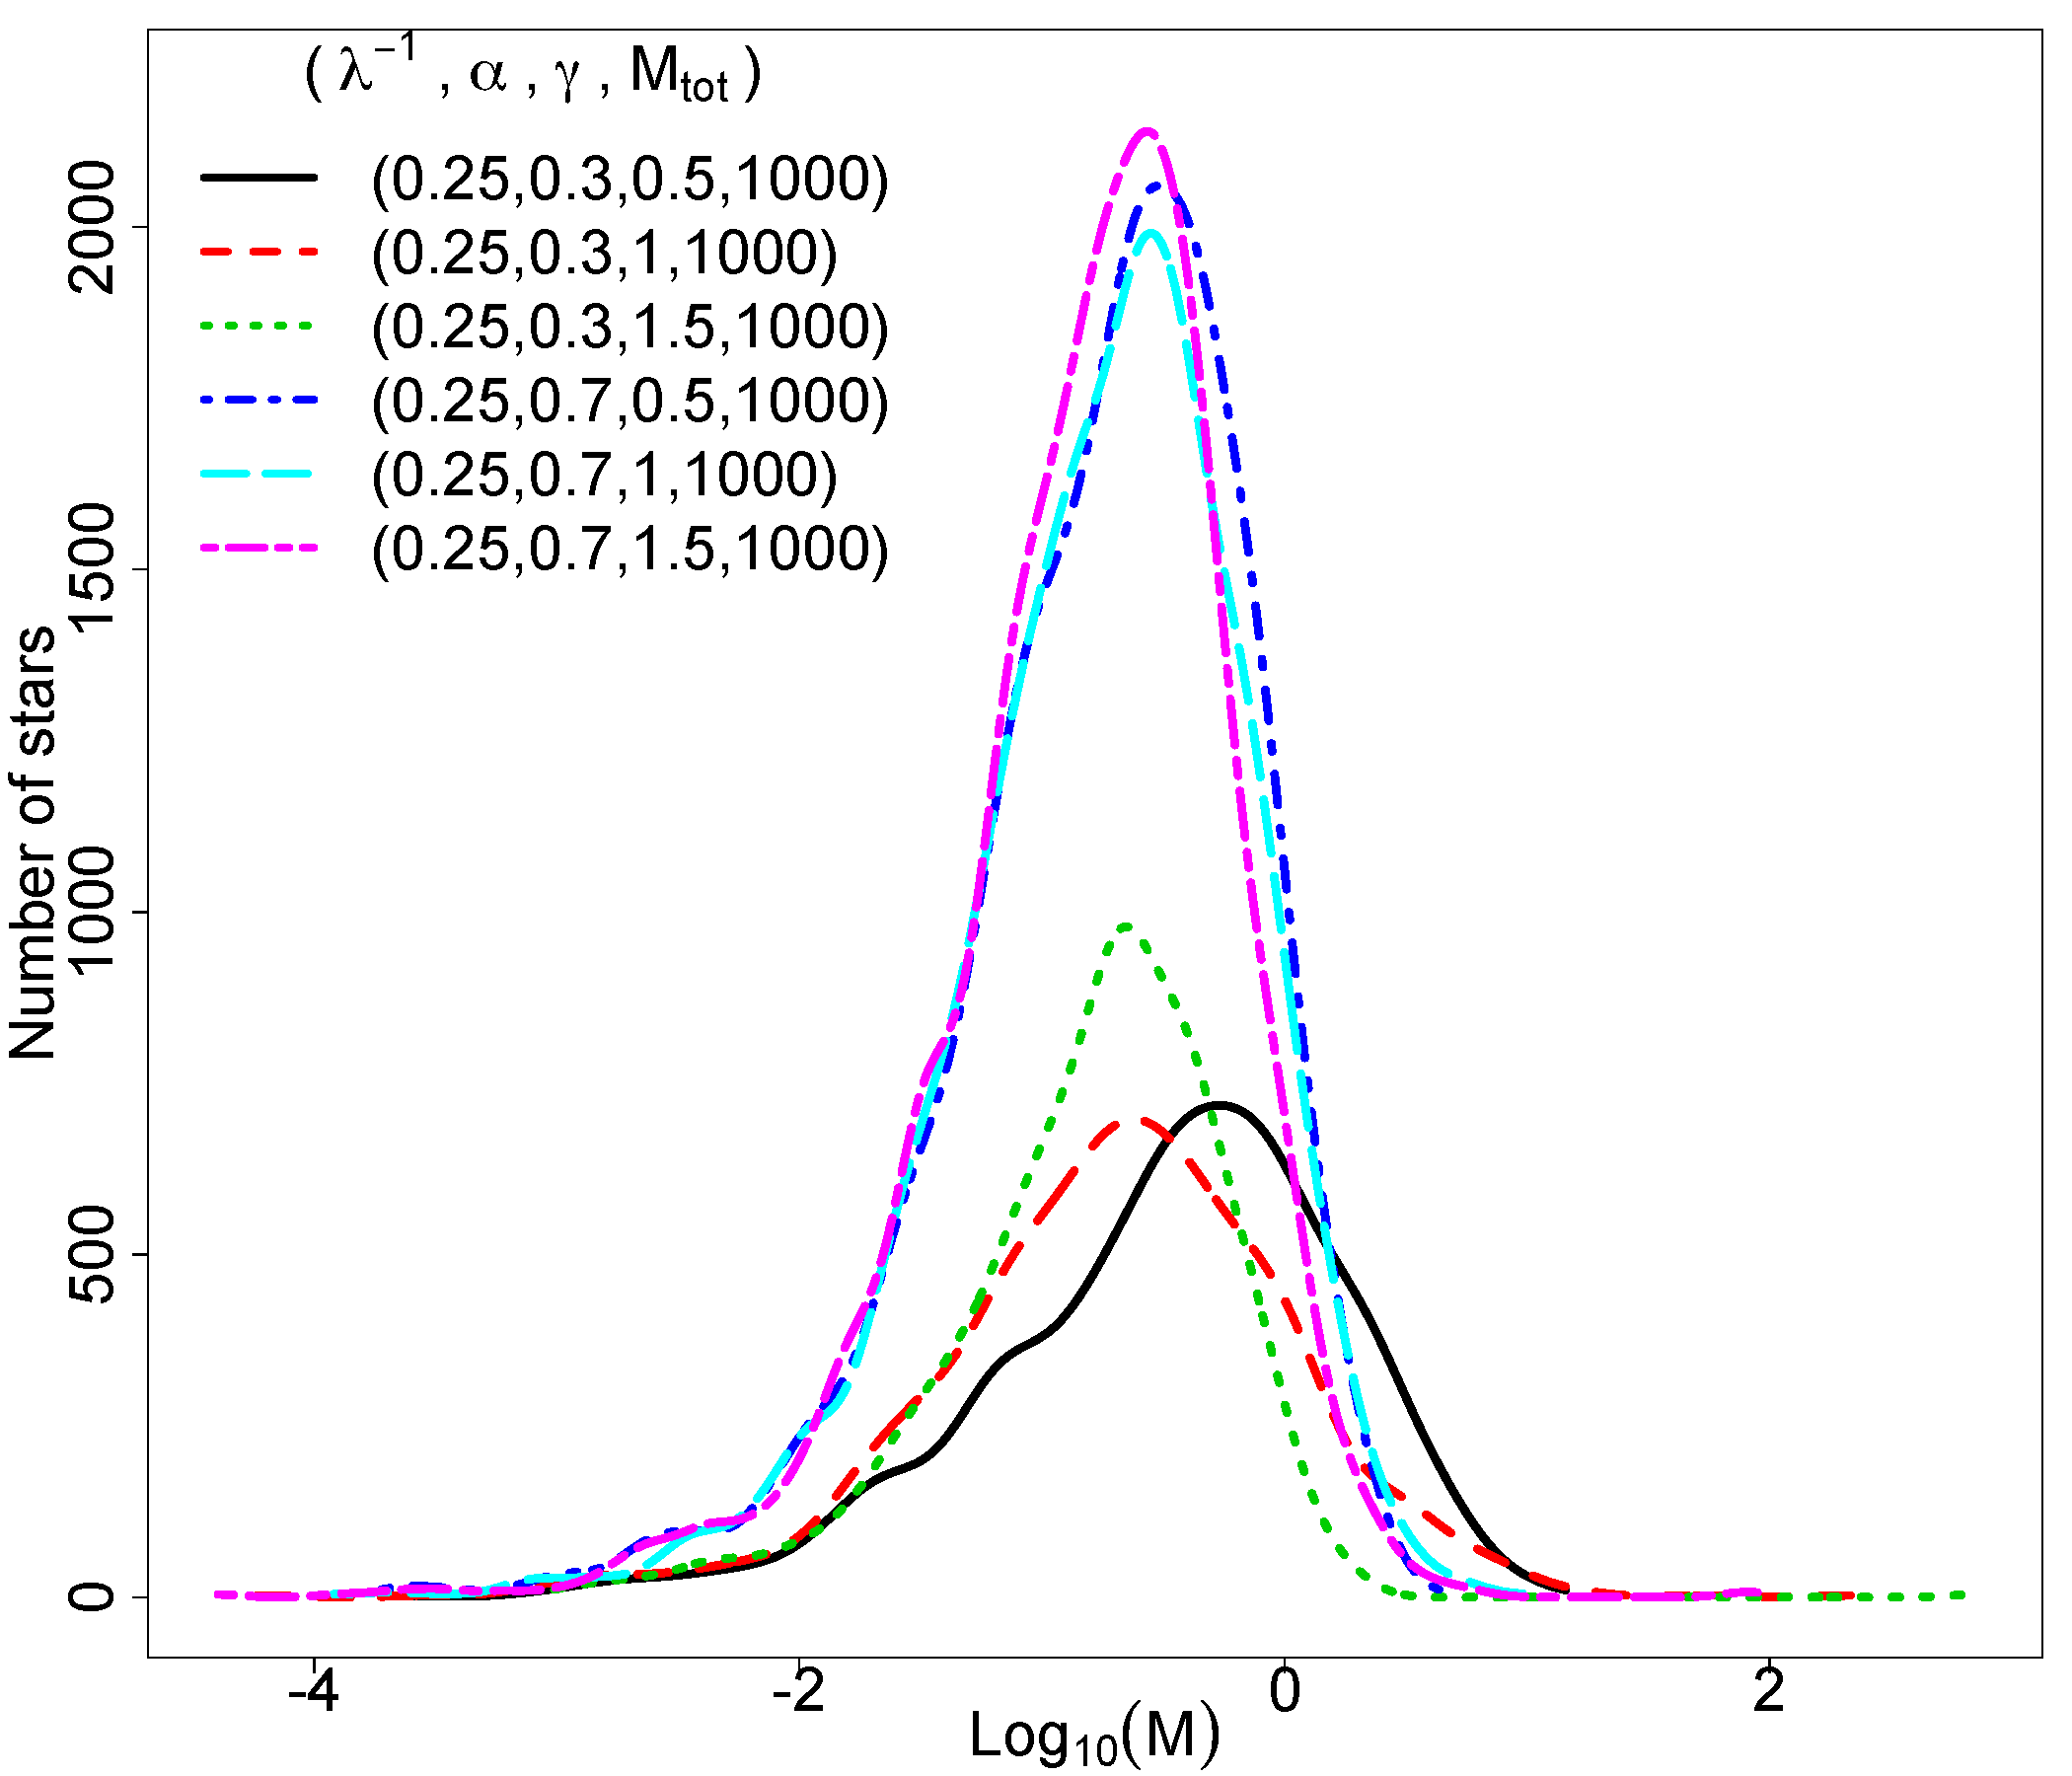
\includegraphics[width = .8\textwidth]{figures/sim_study_true_imf.pdf} 
   \captionof{figure}{The simulated IMF's used as the observations in the simulation study displayed as number of stars by Log$_{10}$ mass.
   }
   \label{fig:true_imf}
\end{minipage}
\end{table}



%
%\begin{table}[htbp]
%   \centering
%   \begin{tabular}{|c|c|c|c|c|} % Column formatting, @{} suppresses leading/trailing space
%   \hline
%   Number & $\lambda^{-1}$ & $\alpha$ & $\gamma$  & $\Mtot$ \\
%   \hline
%1	&	0.25	&	0.3	&	0.5	& 1000 \\
%2	&	0.25	&	0.3	&	1.0	& 1000 \\
%3	&	0.25	&	0.3	&	1.5	& 1000 \\
%4	&	0.25	&	0.7	&	0.5	& 1000 \\
%5	&	0.25	&	0.7	&	1.0	& 1000 \\
%6	&	0.25	&	0.7	&	1.5	& 1000 \\
%\hline
%   \end{tabular}
%   \begin{tabular}{|c|} % Column formatting, @{} suppresses leading/trailing space
%   \hline
% $\nobs$ \\
%   \hline
%1166	 \\
%1142	 \\
%1148	 \\
%2801	 \\
%2698	 \\
%2710	 \\
%\hline
%   \end{tabular}
%   \caption{Parameter values for the simulation study of Section~\ref{methodSec}, along with the number of stars in the data set, $\nobs$.}
%   \label{tab:sim_study}
%\end{table}


The resulting marginal ABC posteriors for $\lambda^{-1}$, $\alpha$, $\gamma$, and $\Mtot$ are displayed in Figure~\ref{fig:abc_pa_posterior}, and the pairwise ABC posterior samples are displayed in Figure~\ref{fig:abc_pa_joints}.  
For $\lambda^{-1}$ and $\Mtot$ (Figure~\ref{subfig:marg_k} and \ref{subfig:marg_mtot}, respectively) cover the input values well with differences in the width of the ABC posteriors.   
%
In general, the marginal ABC posteriors for $\alpha$ and $\gamma$ (Figure~\ref{subfig:marg_alpha} and \ref{subfig:marg_gamma}, respectively) cover the input values of the parameters, but their shapes and widths vary.  
%
For example, the width of the marginal posteriors for $\alpha$ appear to depend on the corresponding value of $\gamma$, where $\gamma = 0.5$ results in the broadest marginal ABC posteriors for the same $\alpha$ input, and $\gamma = 1.5$ results in the narrowest marginal ABC posteriors for the same $\alpha$ input. 
%
\jessi{I'm not really sure why the previous statement happens}
\jessi{Figure~\ref{subfig:joint_gamma_alpha} suggests there may be a degeneracy between $\alpha$ and $\gamma$ for the smaller values of $\gamma$.}
\jessi{There appears to be a degeneracy/correlation/dependency between  $\lambda^{-1}$ and $\alpha$, as displayed in Figure~\ref{subfig:joint_alpha_k}.  This makes sense because $\lambda^{-1}$ controls the size of the mass pieces and $\alpha$ controls how many of those mass pieces form new stars; a bigger mass piece EXPLAIN???}
%

The pattern for $\gamma$ is a bit more complicated.  
The marginal posteriors for $\gamma \leq 1$ appear to be narrower with smaller $\alpha$.  
This makes sense because a smaller $\alpha$ results in fewer new stars, which means the entering piece of mass has to join an already formed star, at a rate controlled by the value of $\gamma$.  Hence, more pieces that have to be assigned to existing stars seems to result in more information about the rate of growth of the stars.
However, for a  $\gamma > 1$, a larger $\alpha$ (producing more new stars) appears to lead to a narrower marginal ABC posterior for $\gamma$ than when $\alpha$ is larger (0.7).  
The marginal ABC posterior for $\gamma = 1.5$ corresponding to the smaller value for $\alpha$ (0.3) is wider and pushes against the boundary of the prior.  It turns out that this behavior seems to occur because when $\gamma$ is greater than 1 and $\alpha$ is smaller, all the mass that has to be distributed to the already existing stars (rather than forming a new star) tends to be assigned to the same, most massive star.  There ends up a being a runaway effect in this scenario ($\gamma > 1$ and smaller $\alpha$) where almost all of the incoming mass is assigned to the same star, resulting in one extremely massive star.  This means there is essentially only one star for providing information on the $\gamma$, which may be why the ABC posterior is wider and pushes against the upper boundary of the prior on $\gamma$.





\begin{figure}[htbp]
   \centering
%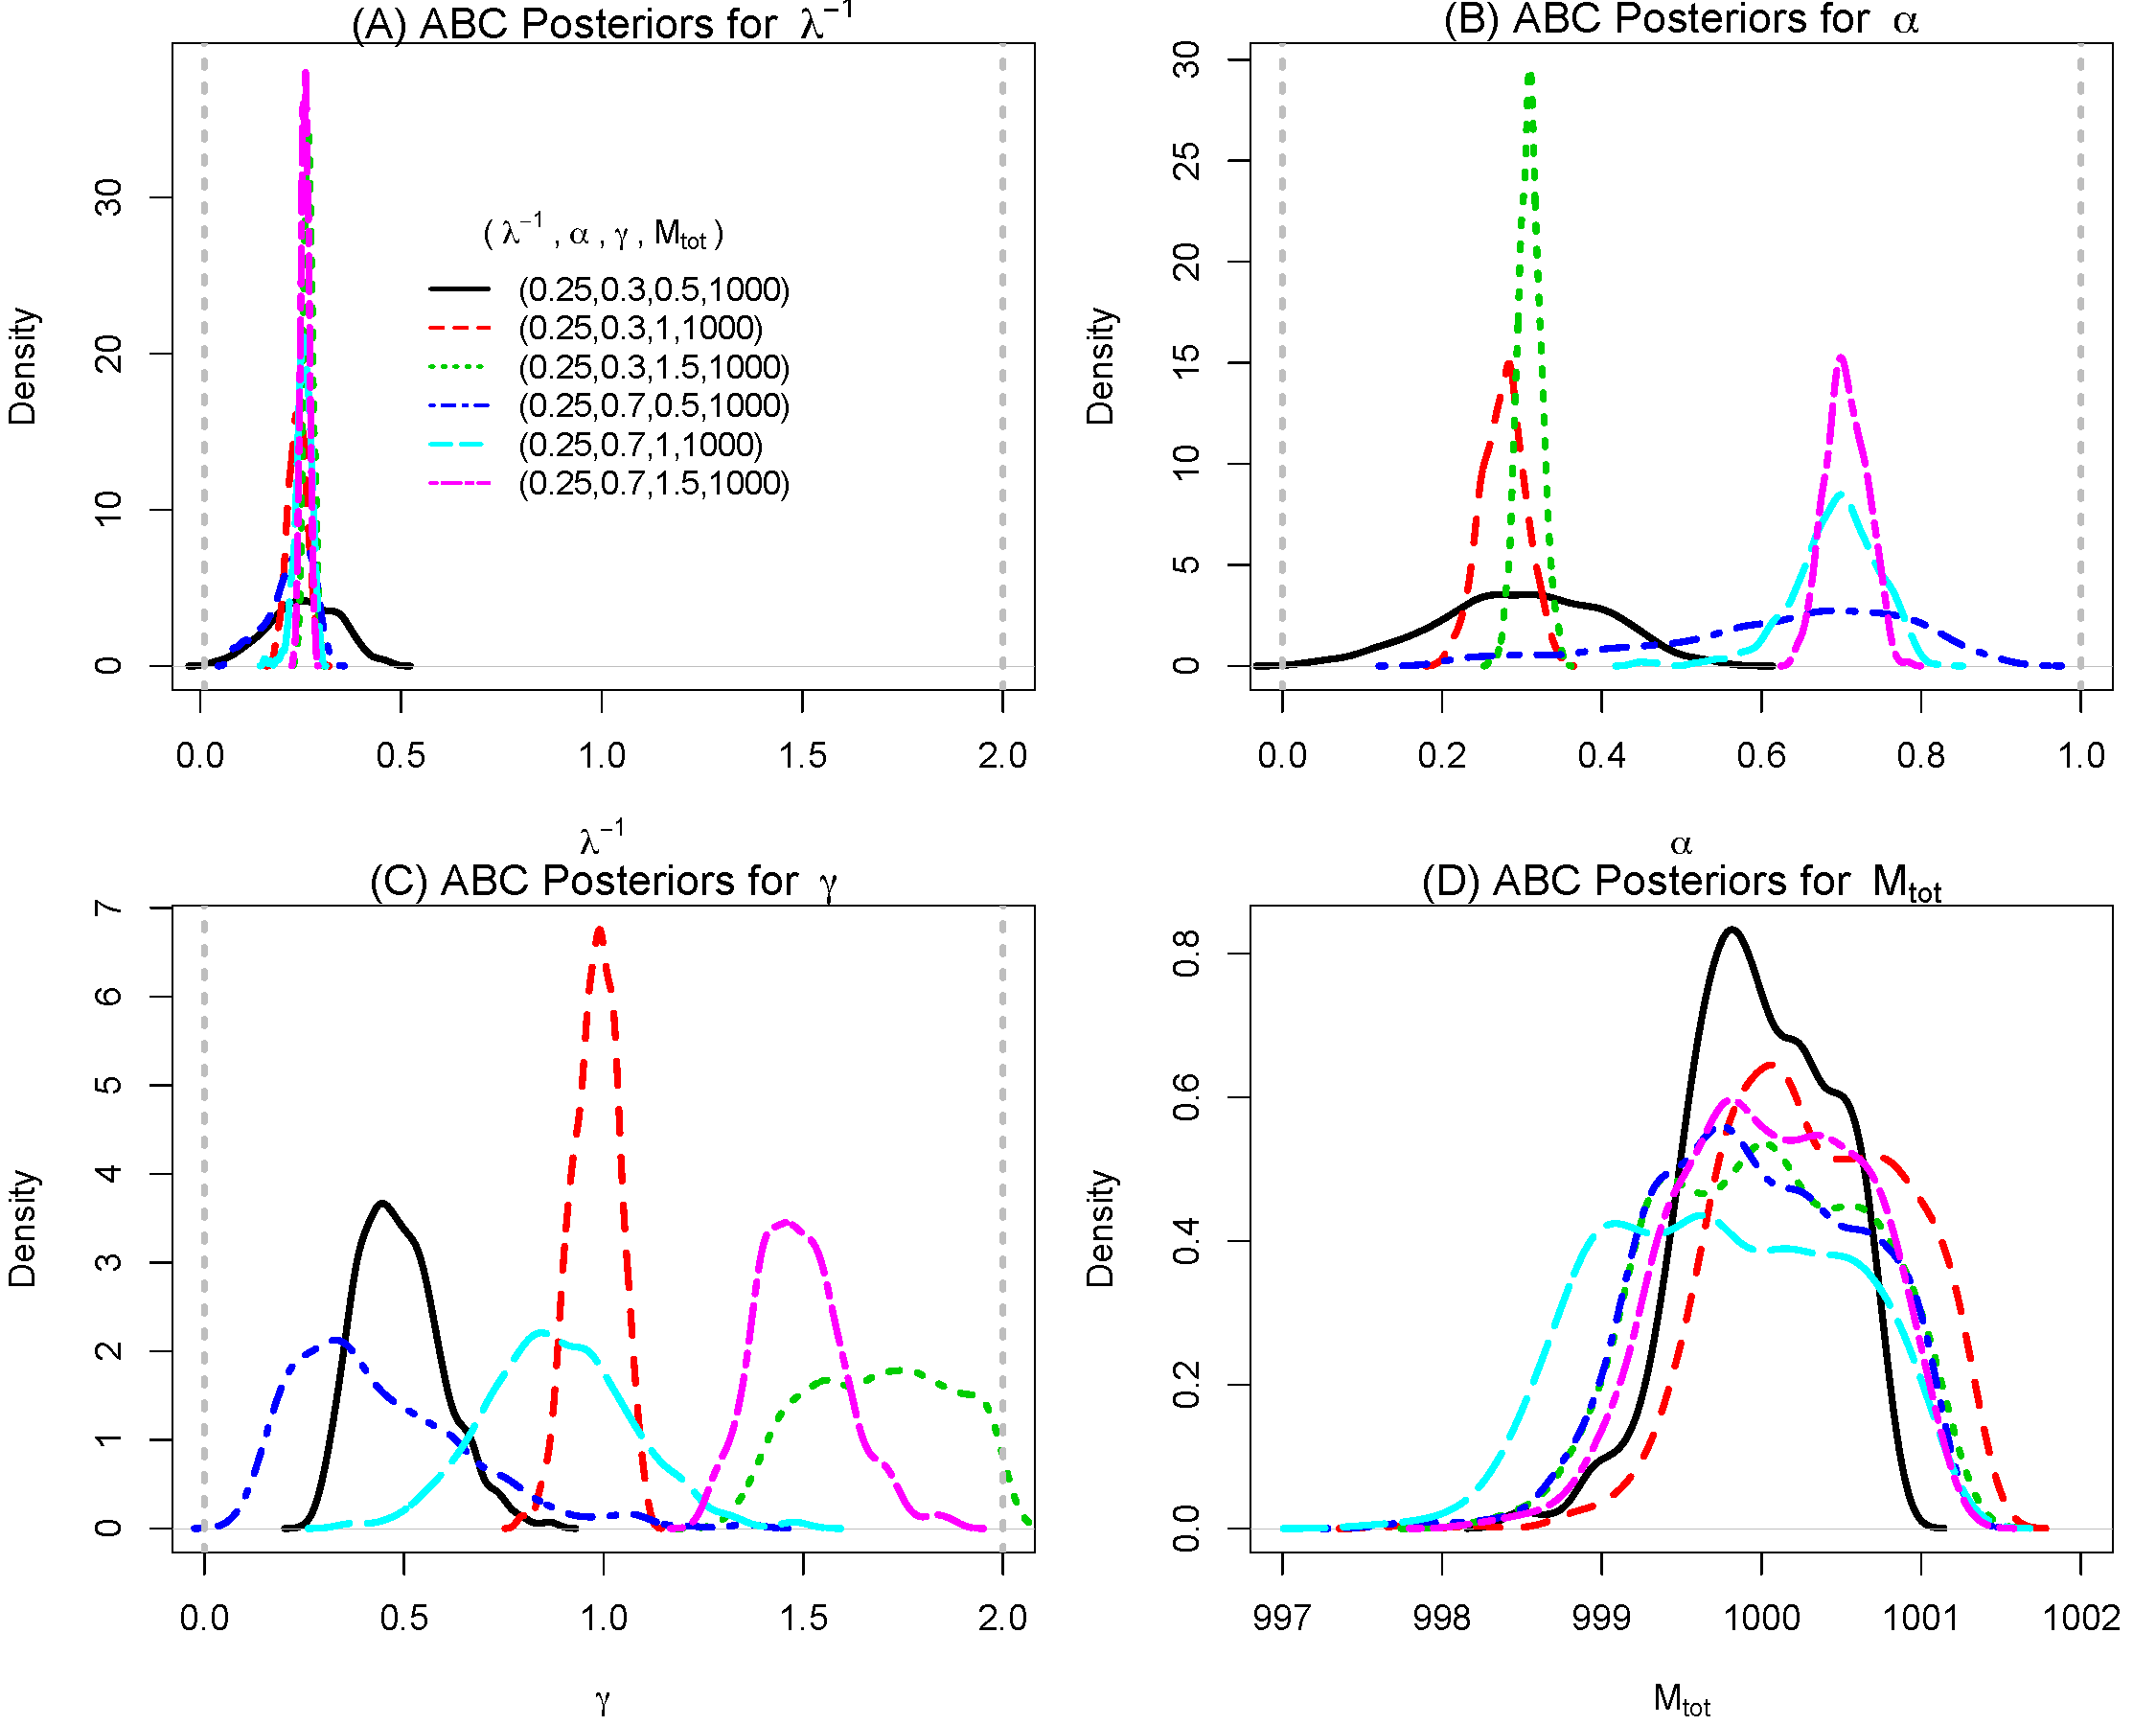
\includegraphics[width = .95\textwidth]{figures/sim_study_marginals.pdf} 
\begin{subfigure}{0.48\textwidth}
\centering
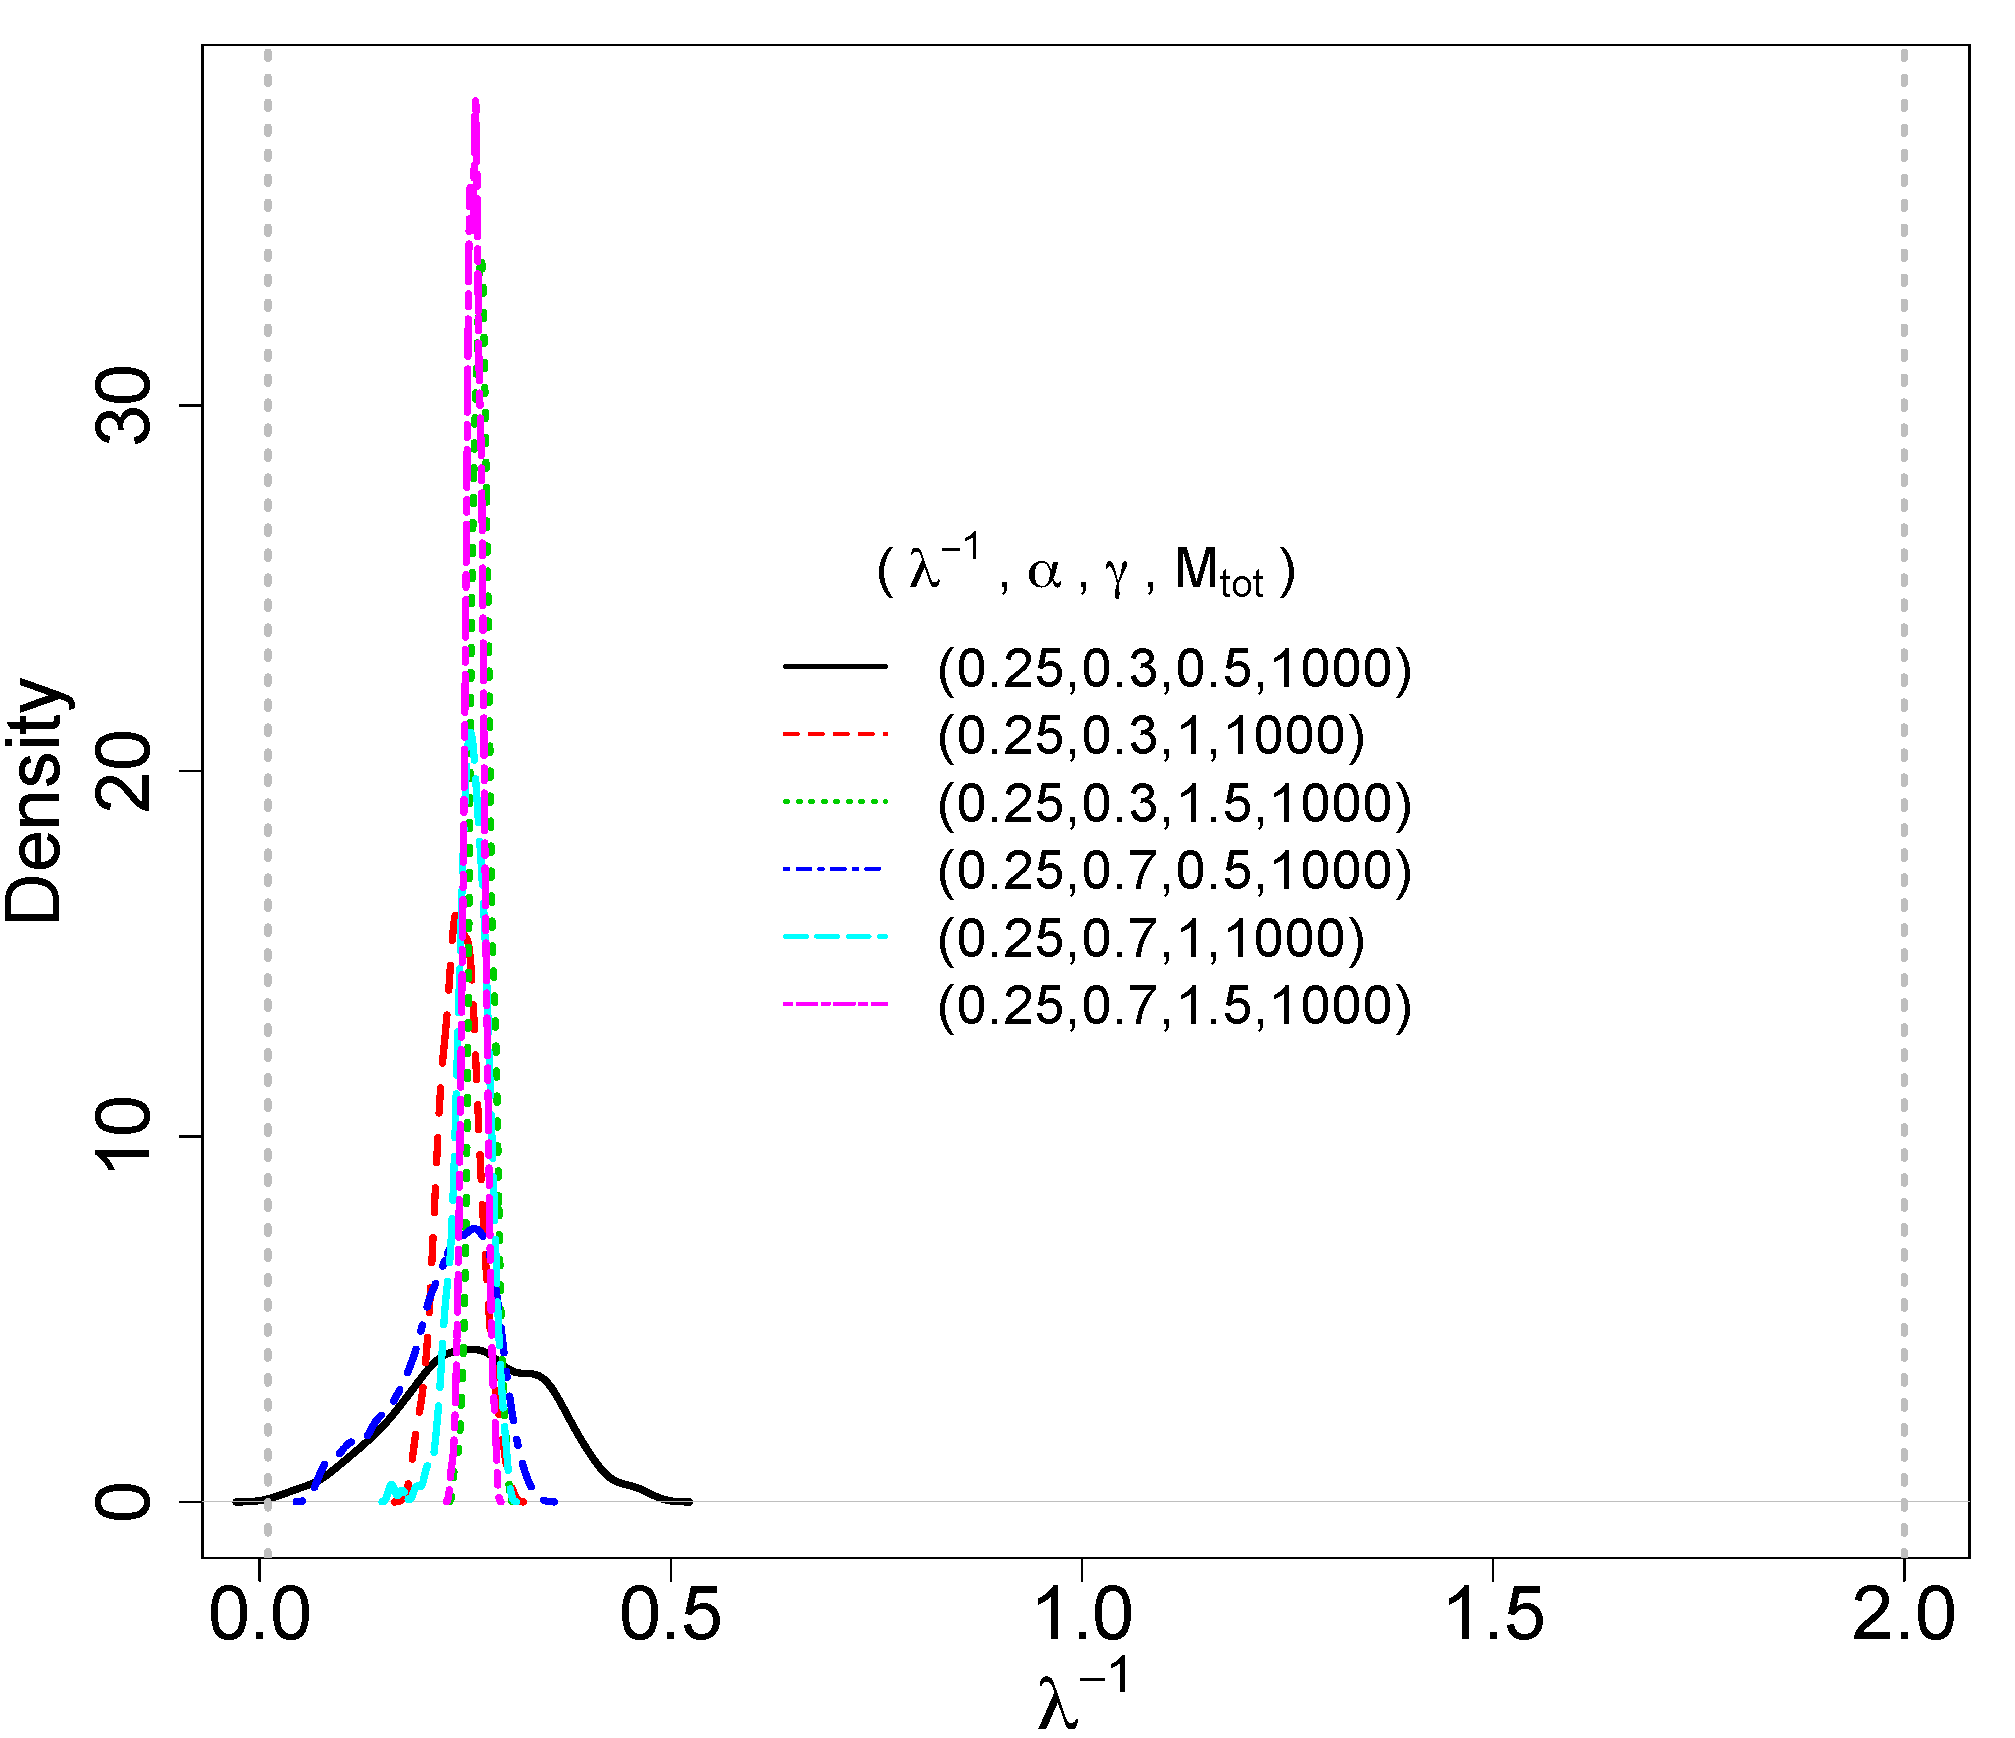
\includegraphics[width = \textwidth]{figures/marg_k.pdf} 
\caption{ABC marginal posterior for $\lambda^{-1}$}\label{subfig:marg_k}
\end{subfigure}
\begin{subfigure}{0.48\textwidth}
\centering
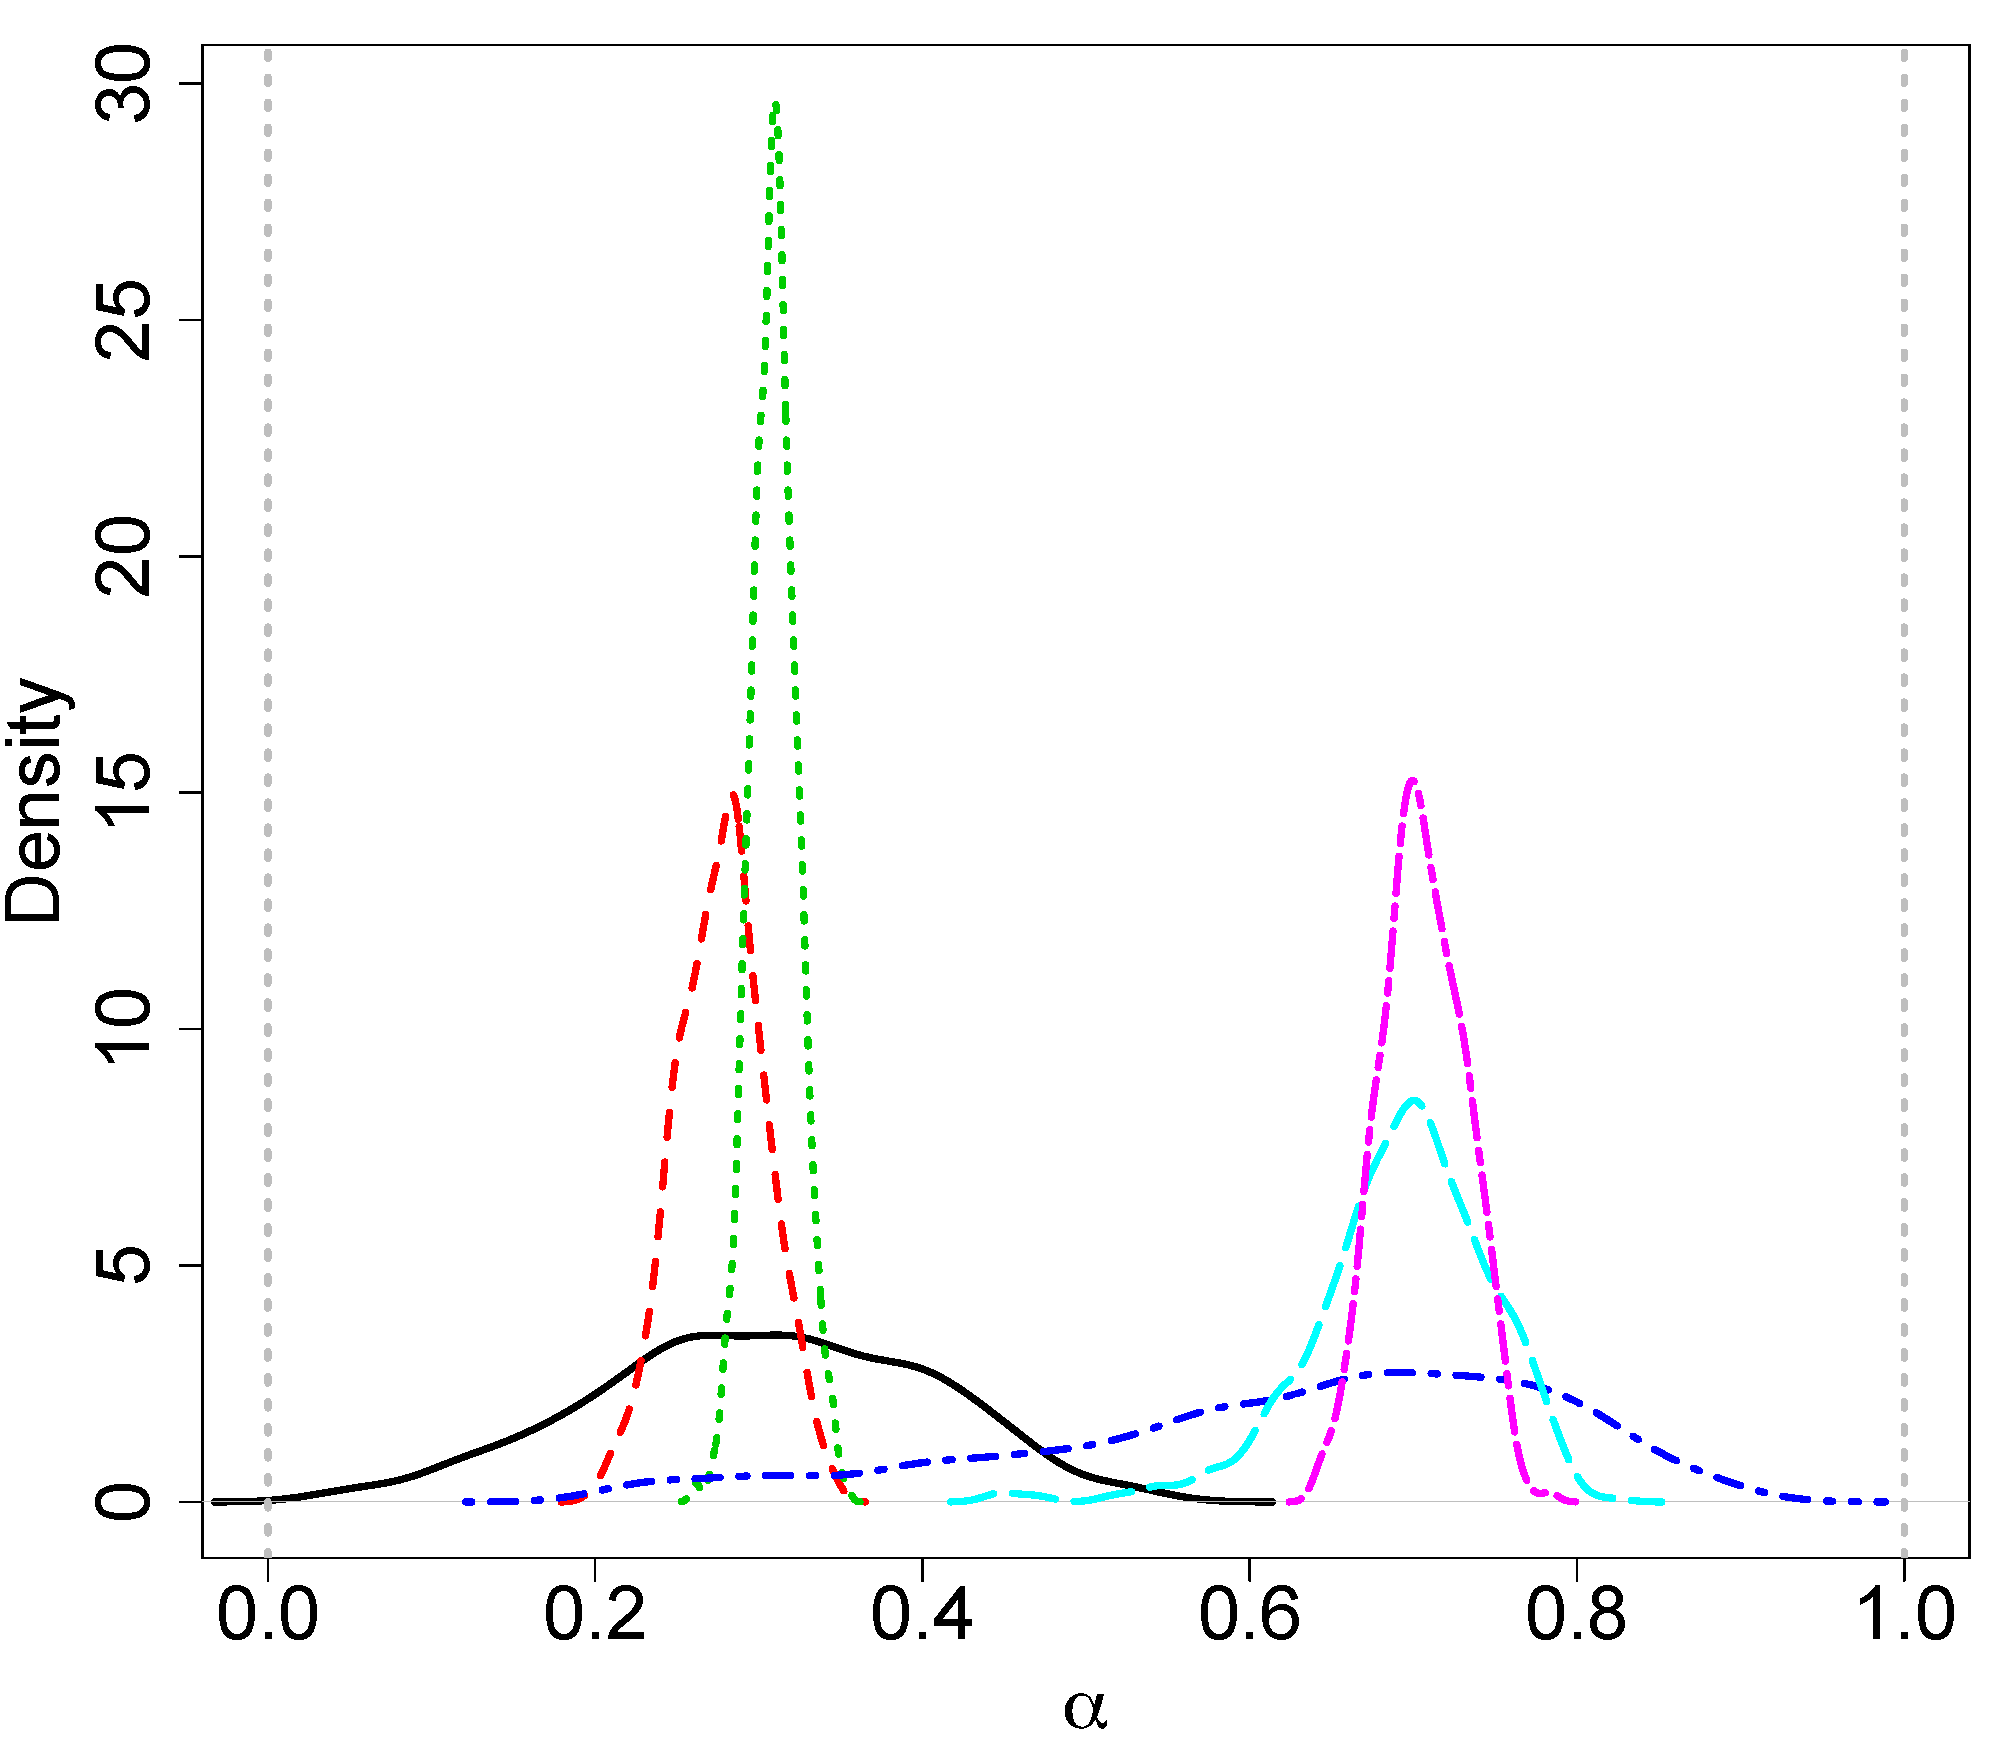
\includegraphics[width = \textwidth]{figures/marg_alpha.pdf} 
\caption{ABC marginal posterior for  $\alpha$}\label{subfig:marg_alpha} 
\end{subfigure} \\
\begin{subfigure}{0.48\textwidth}
\centering
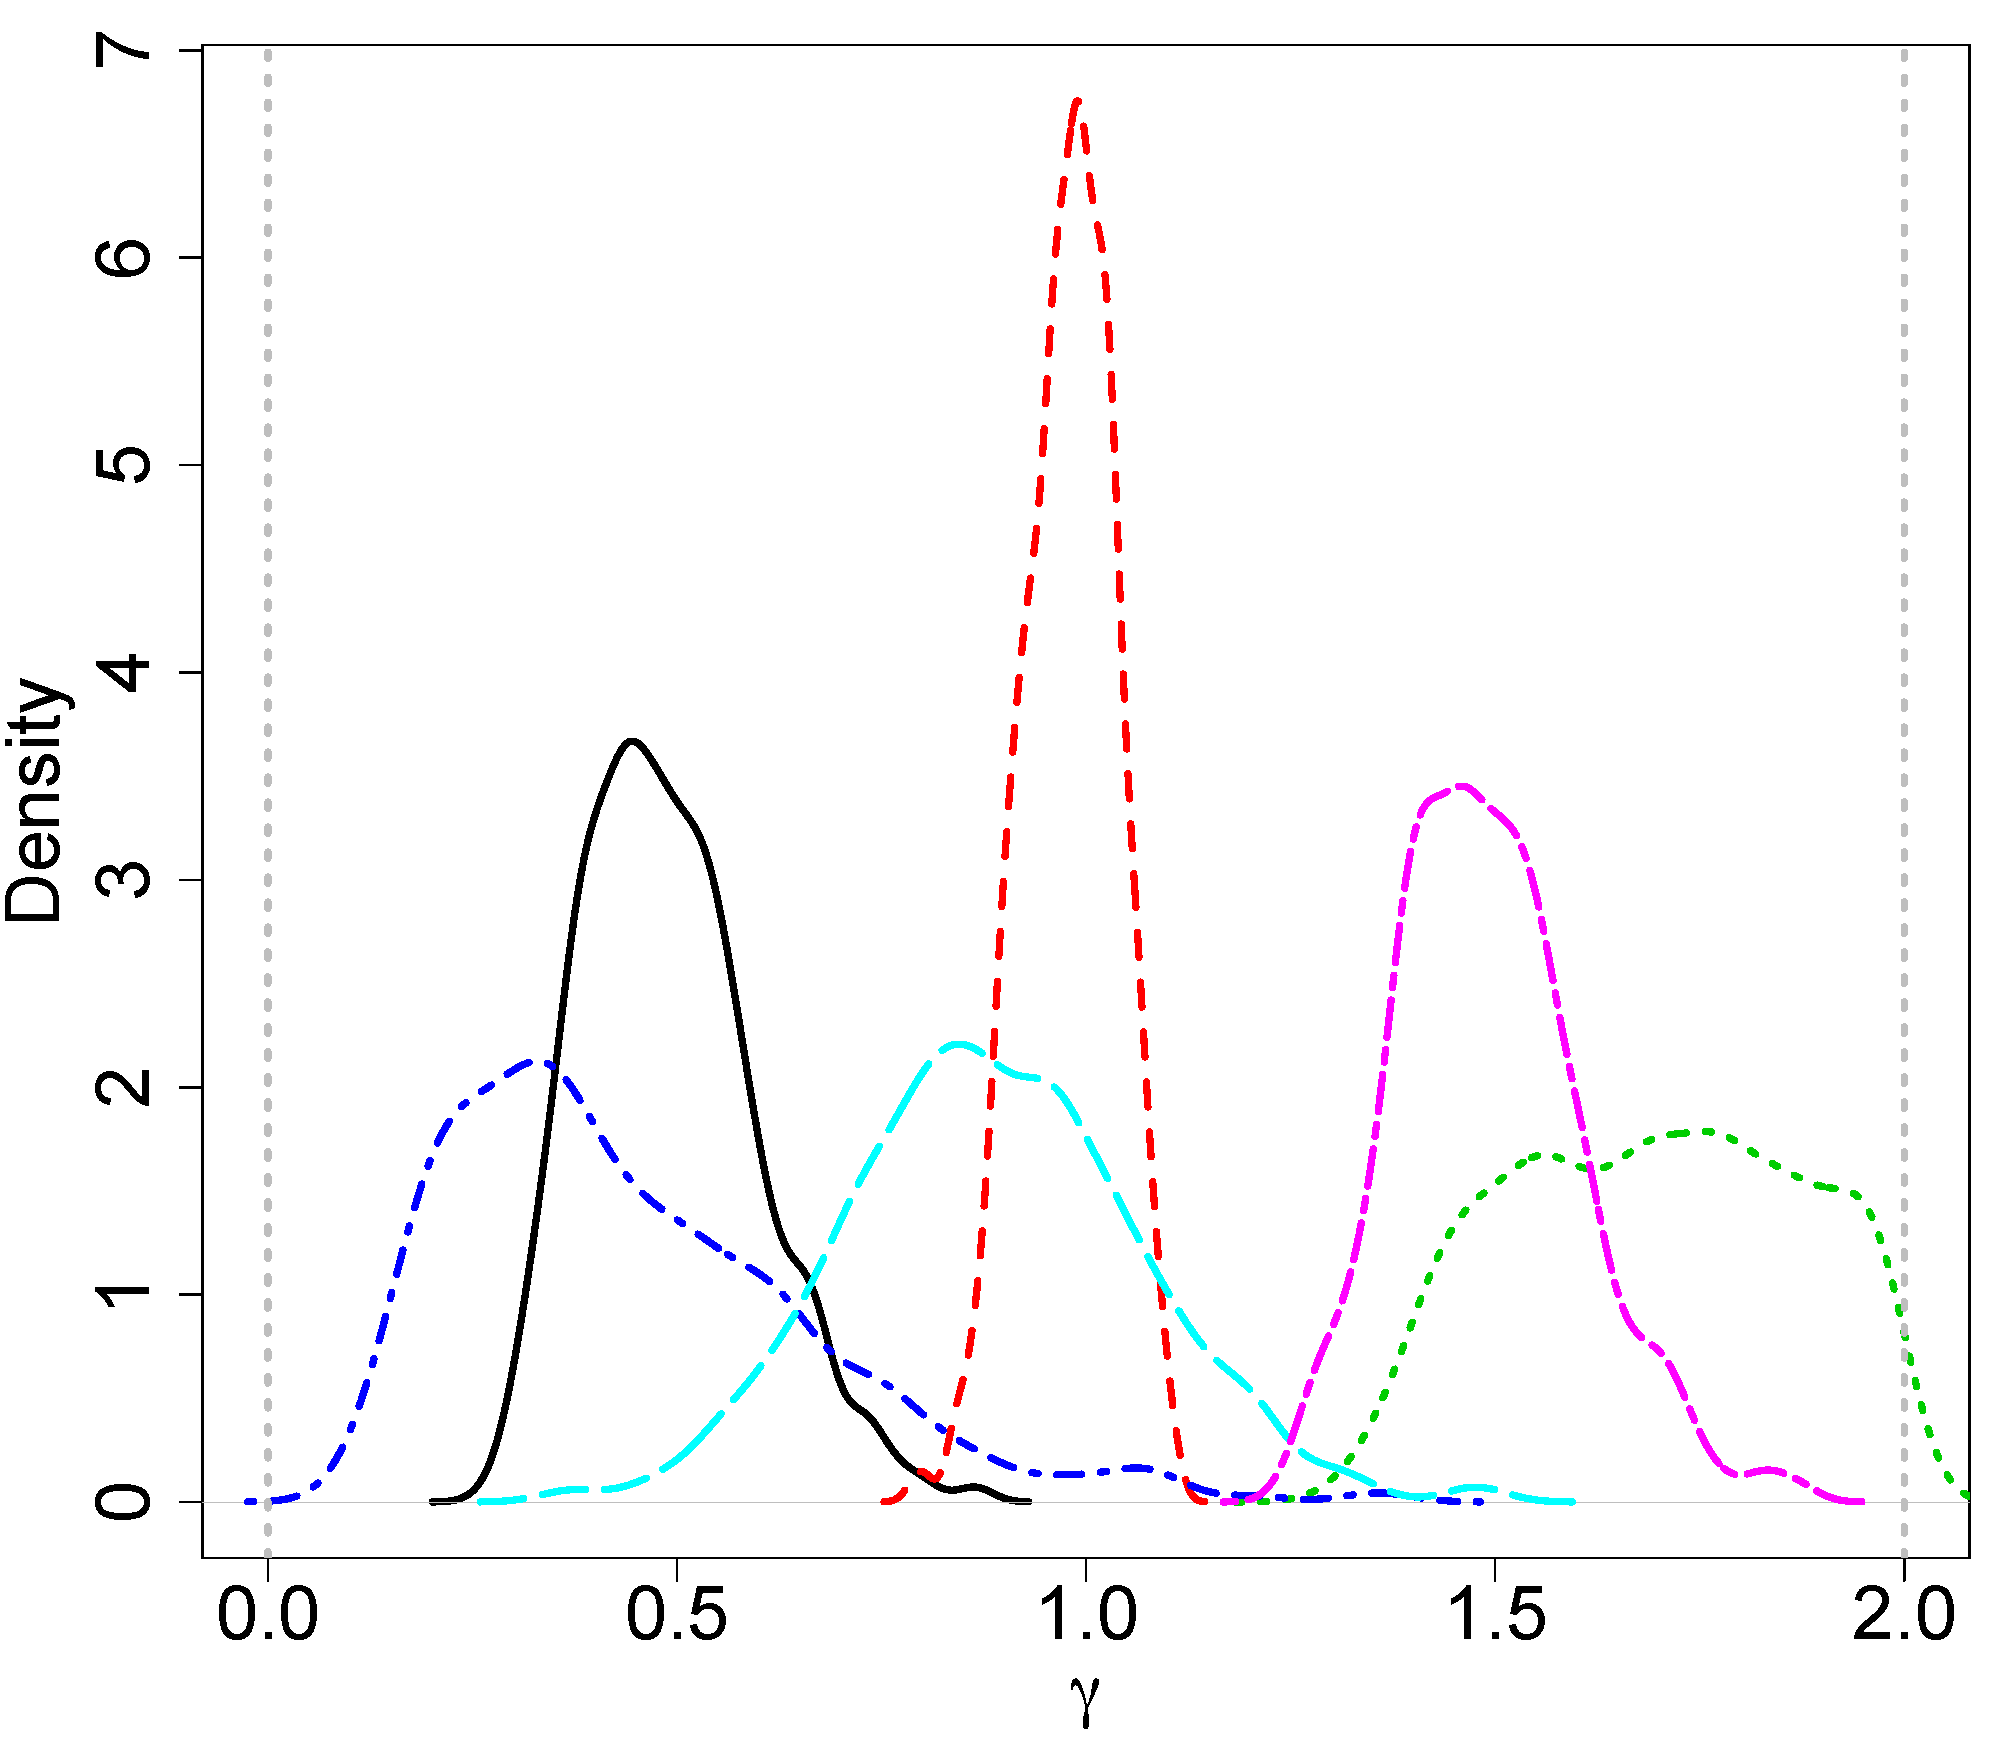
\includegraphics[width = \textwidth]{figures/marg_gamma.pdf} 
\caption{ABC marginal posterior for $\gamma$}\label{subfig:marg_gamma}
\end{subfigure}
\begin{subfigure}{0.48\textwidth}
\centering
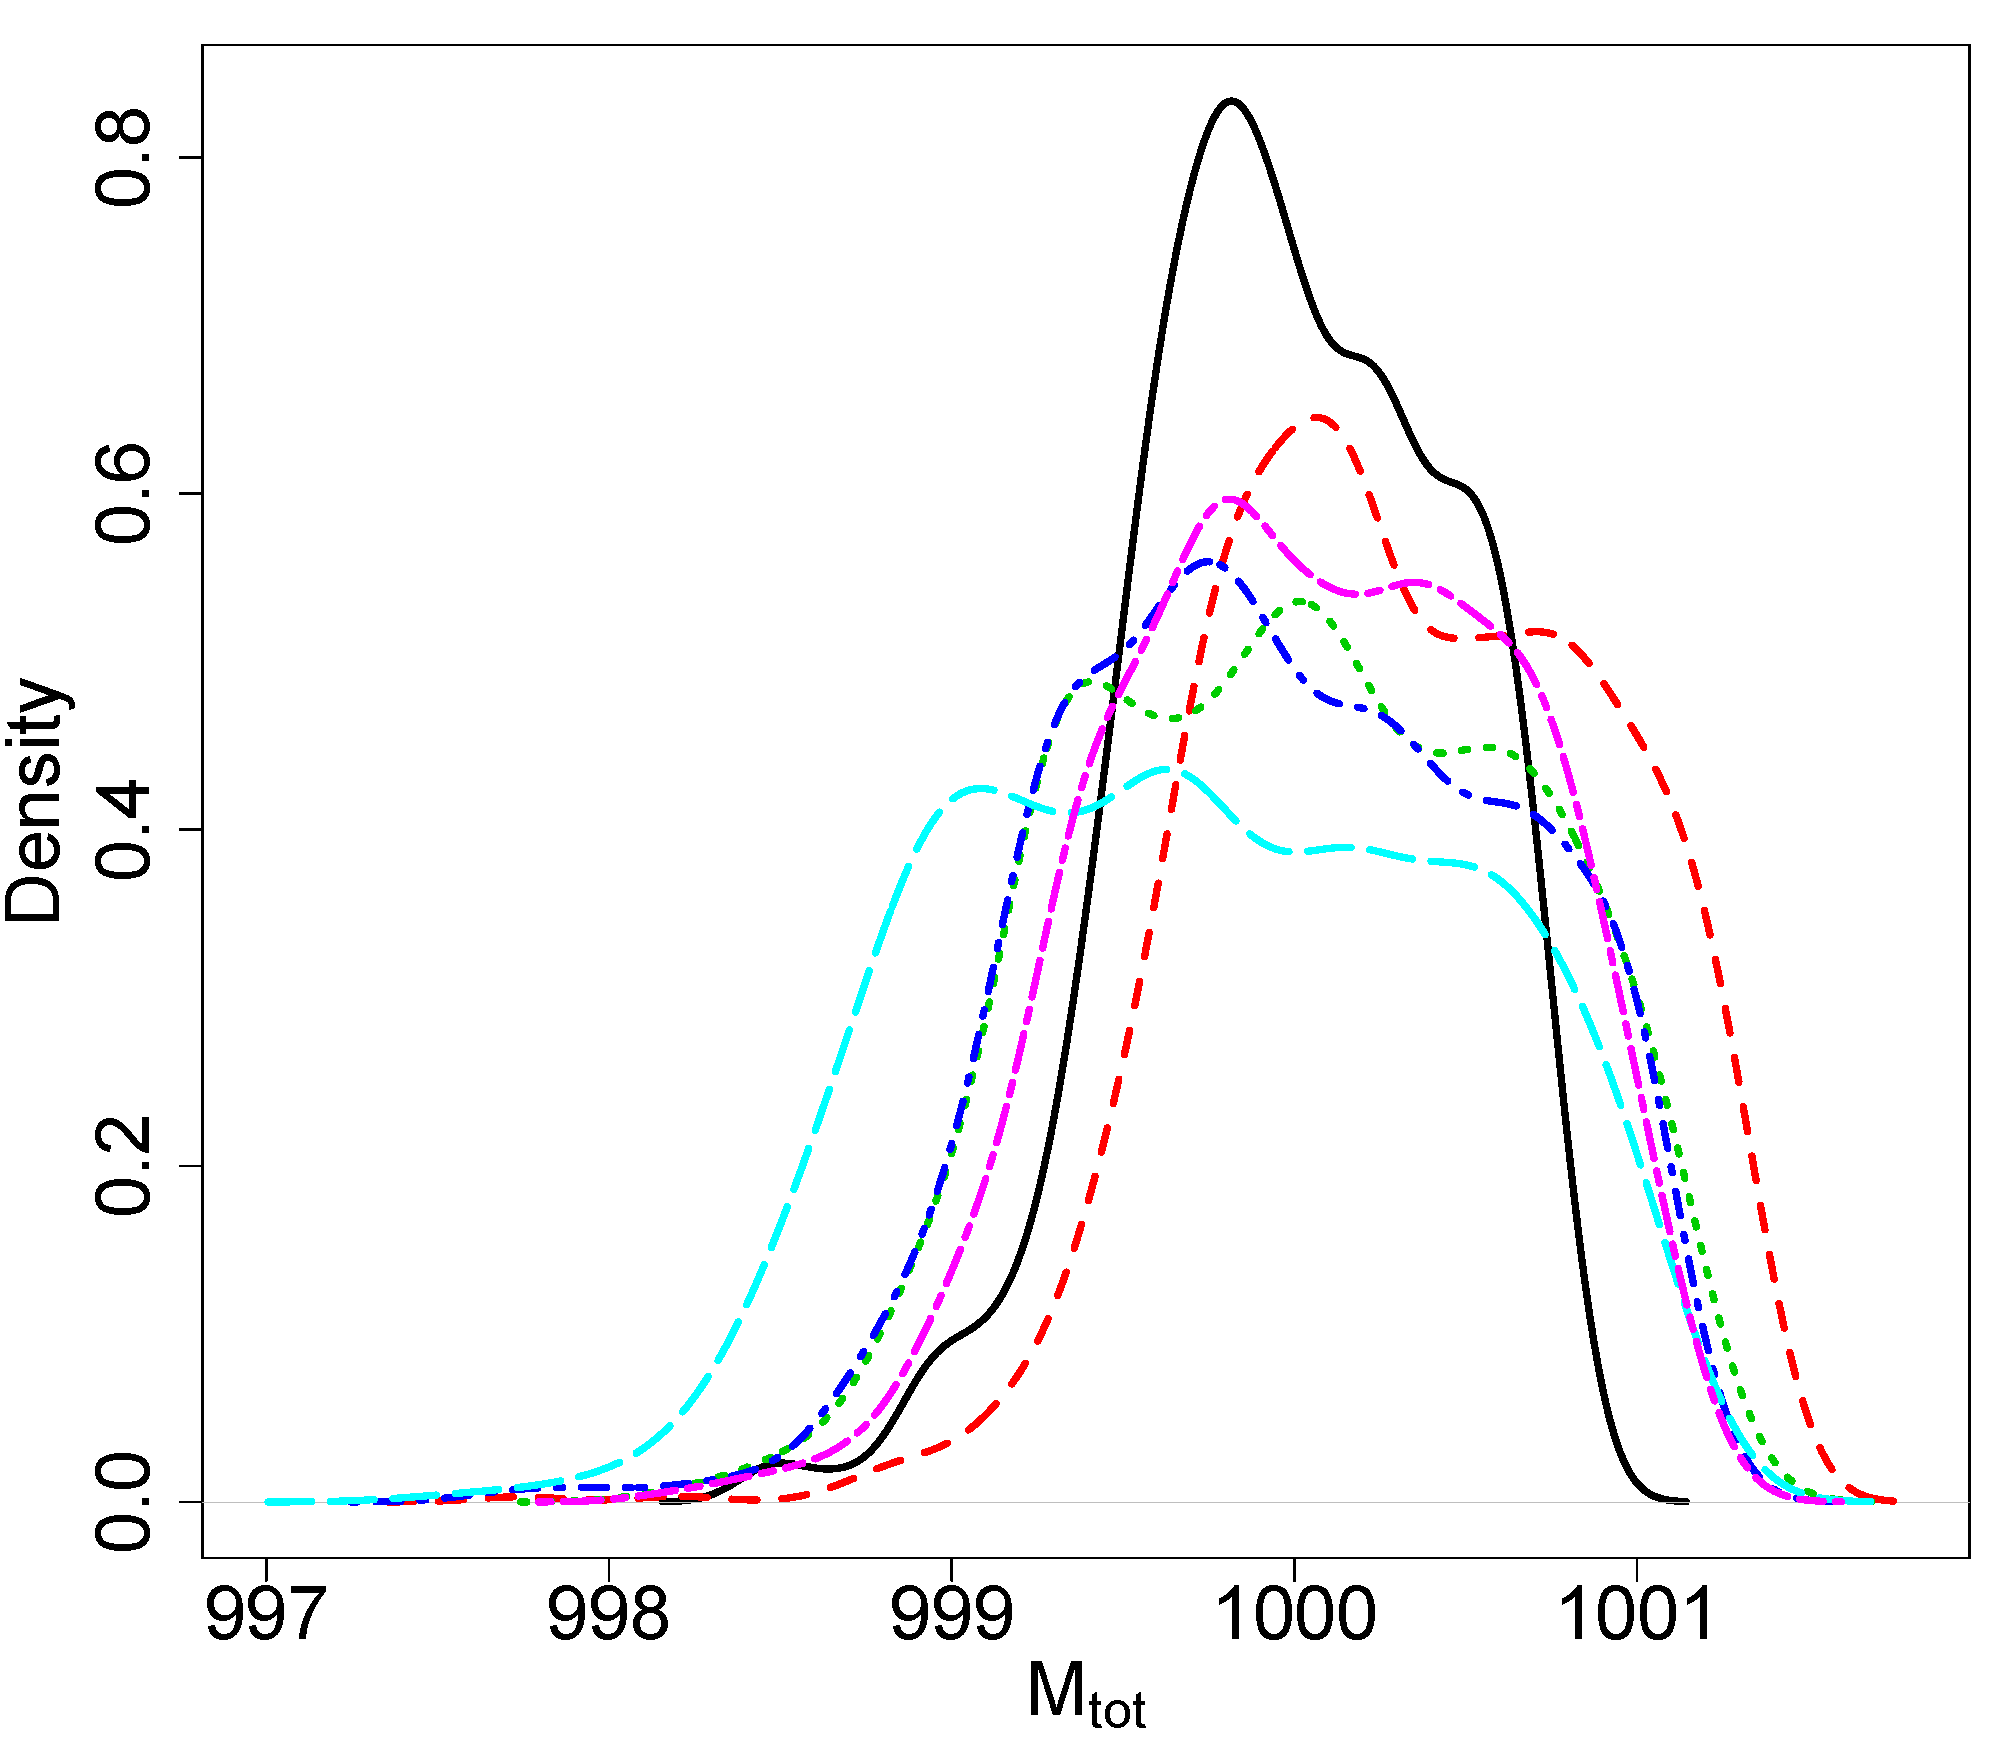
\includegraphics[width = \textwidth]{figures/marg_mtot.pdf} 
\caption{ABC marginal posterior for  $\Mtot$}\label{subfig:marg_mtot}
\end{subfigure}
%
 \caption{Marginal ABC posteriors for the simulation settings of Table~\ref{tab:sim_study}.  The different color and types of lines indicate the input parameter values corresponding to the weighted kernel density estimates of the marginal ABC posteriors for (a) $\lambda^{-1}$, (b) $\alpha$, (c) $\gamma$, and (d) $\Mtot$.  The vertical dotted gray lines in plots (a) - (c) indicate the range of the uniform prior for the parameter.  The prior used for $\Mtot$ was a Normal distribution with a prior mean of 1200 and a prior standard deviation of 600.
   }
   \label{fig:abc_pa_posterior}
\end{figure}


\begin{figure}[htbp]
   \centering
\begin{subfigure}{0.32\textwidth}
\centering
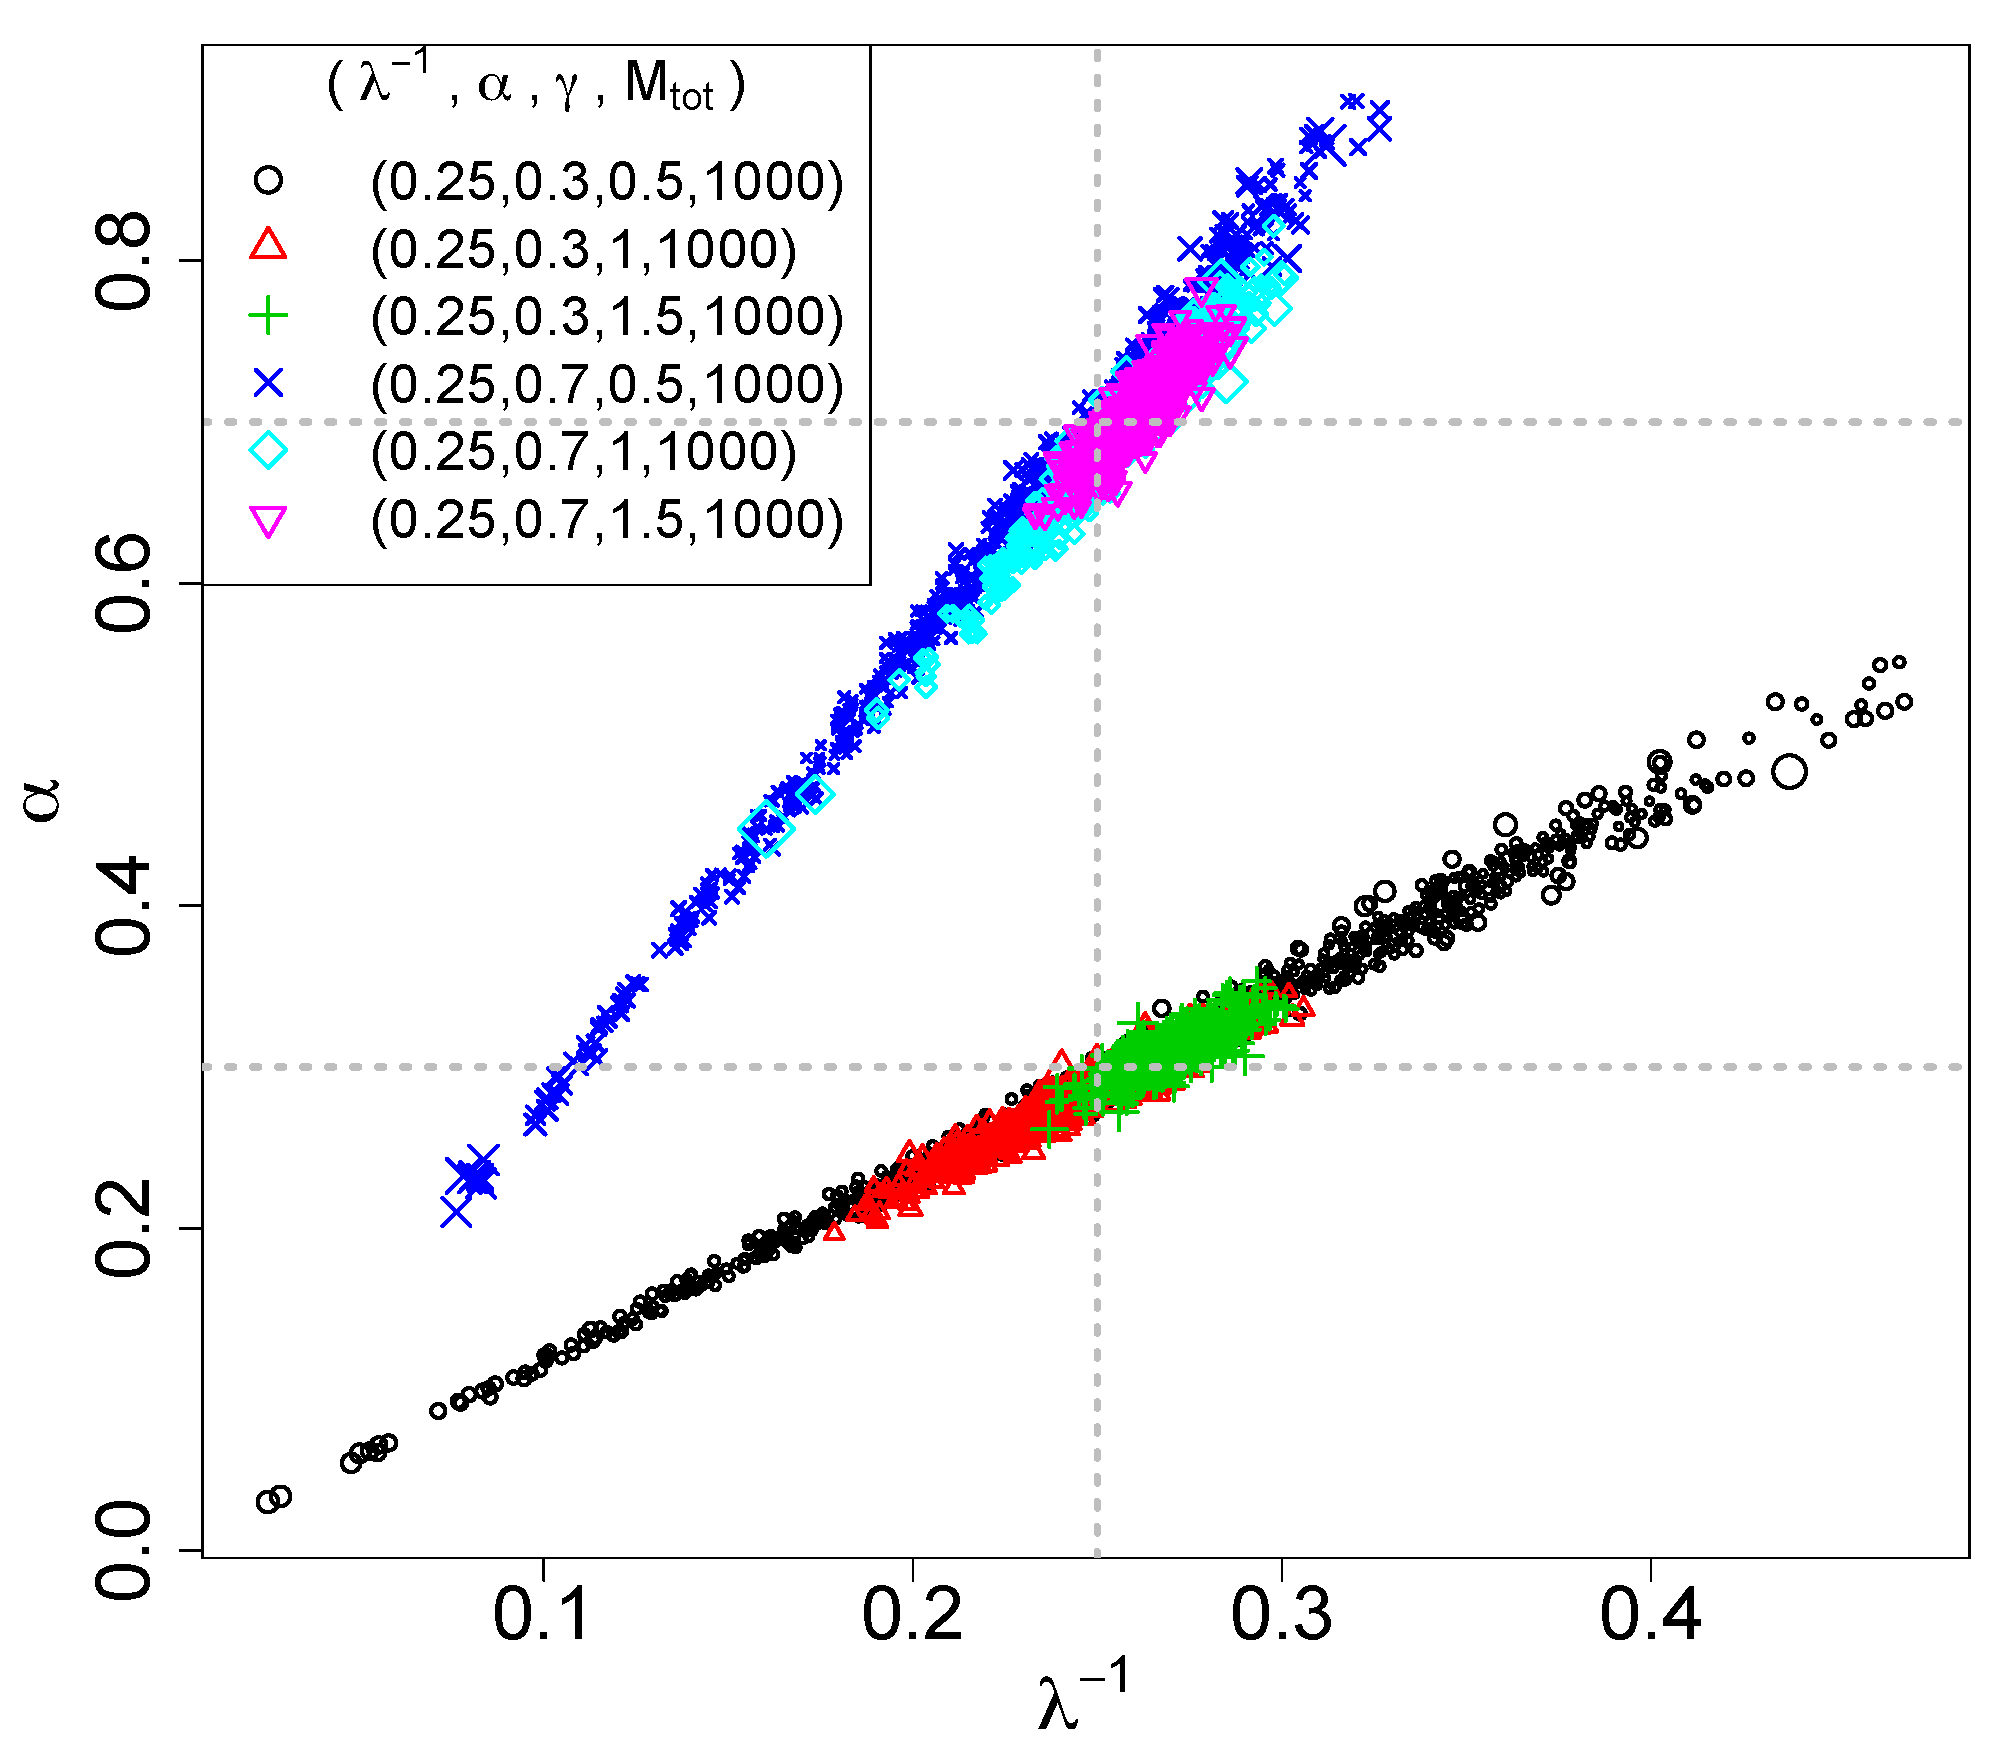
\includegraphics[width = \textwidth]{figures/joint_k_alpha.pdf} 
\caption{ABC Joint $(\lambda^{-1}, \alpha)$}\label{subfig:joint_alpha_k}
\end{subfigure}
\begin{subfigure}{0.32\textwidth}
\centering
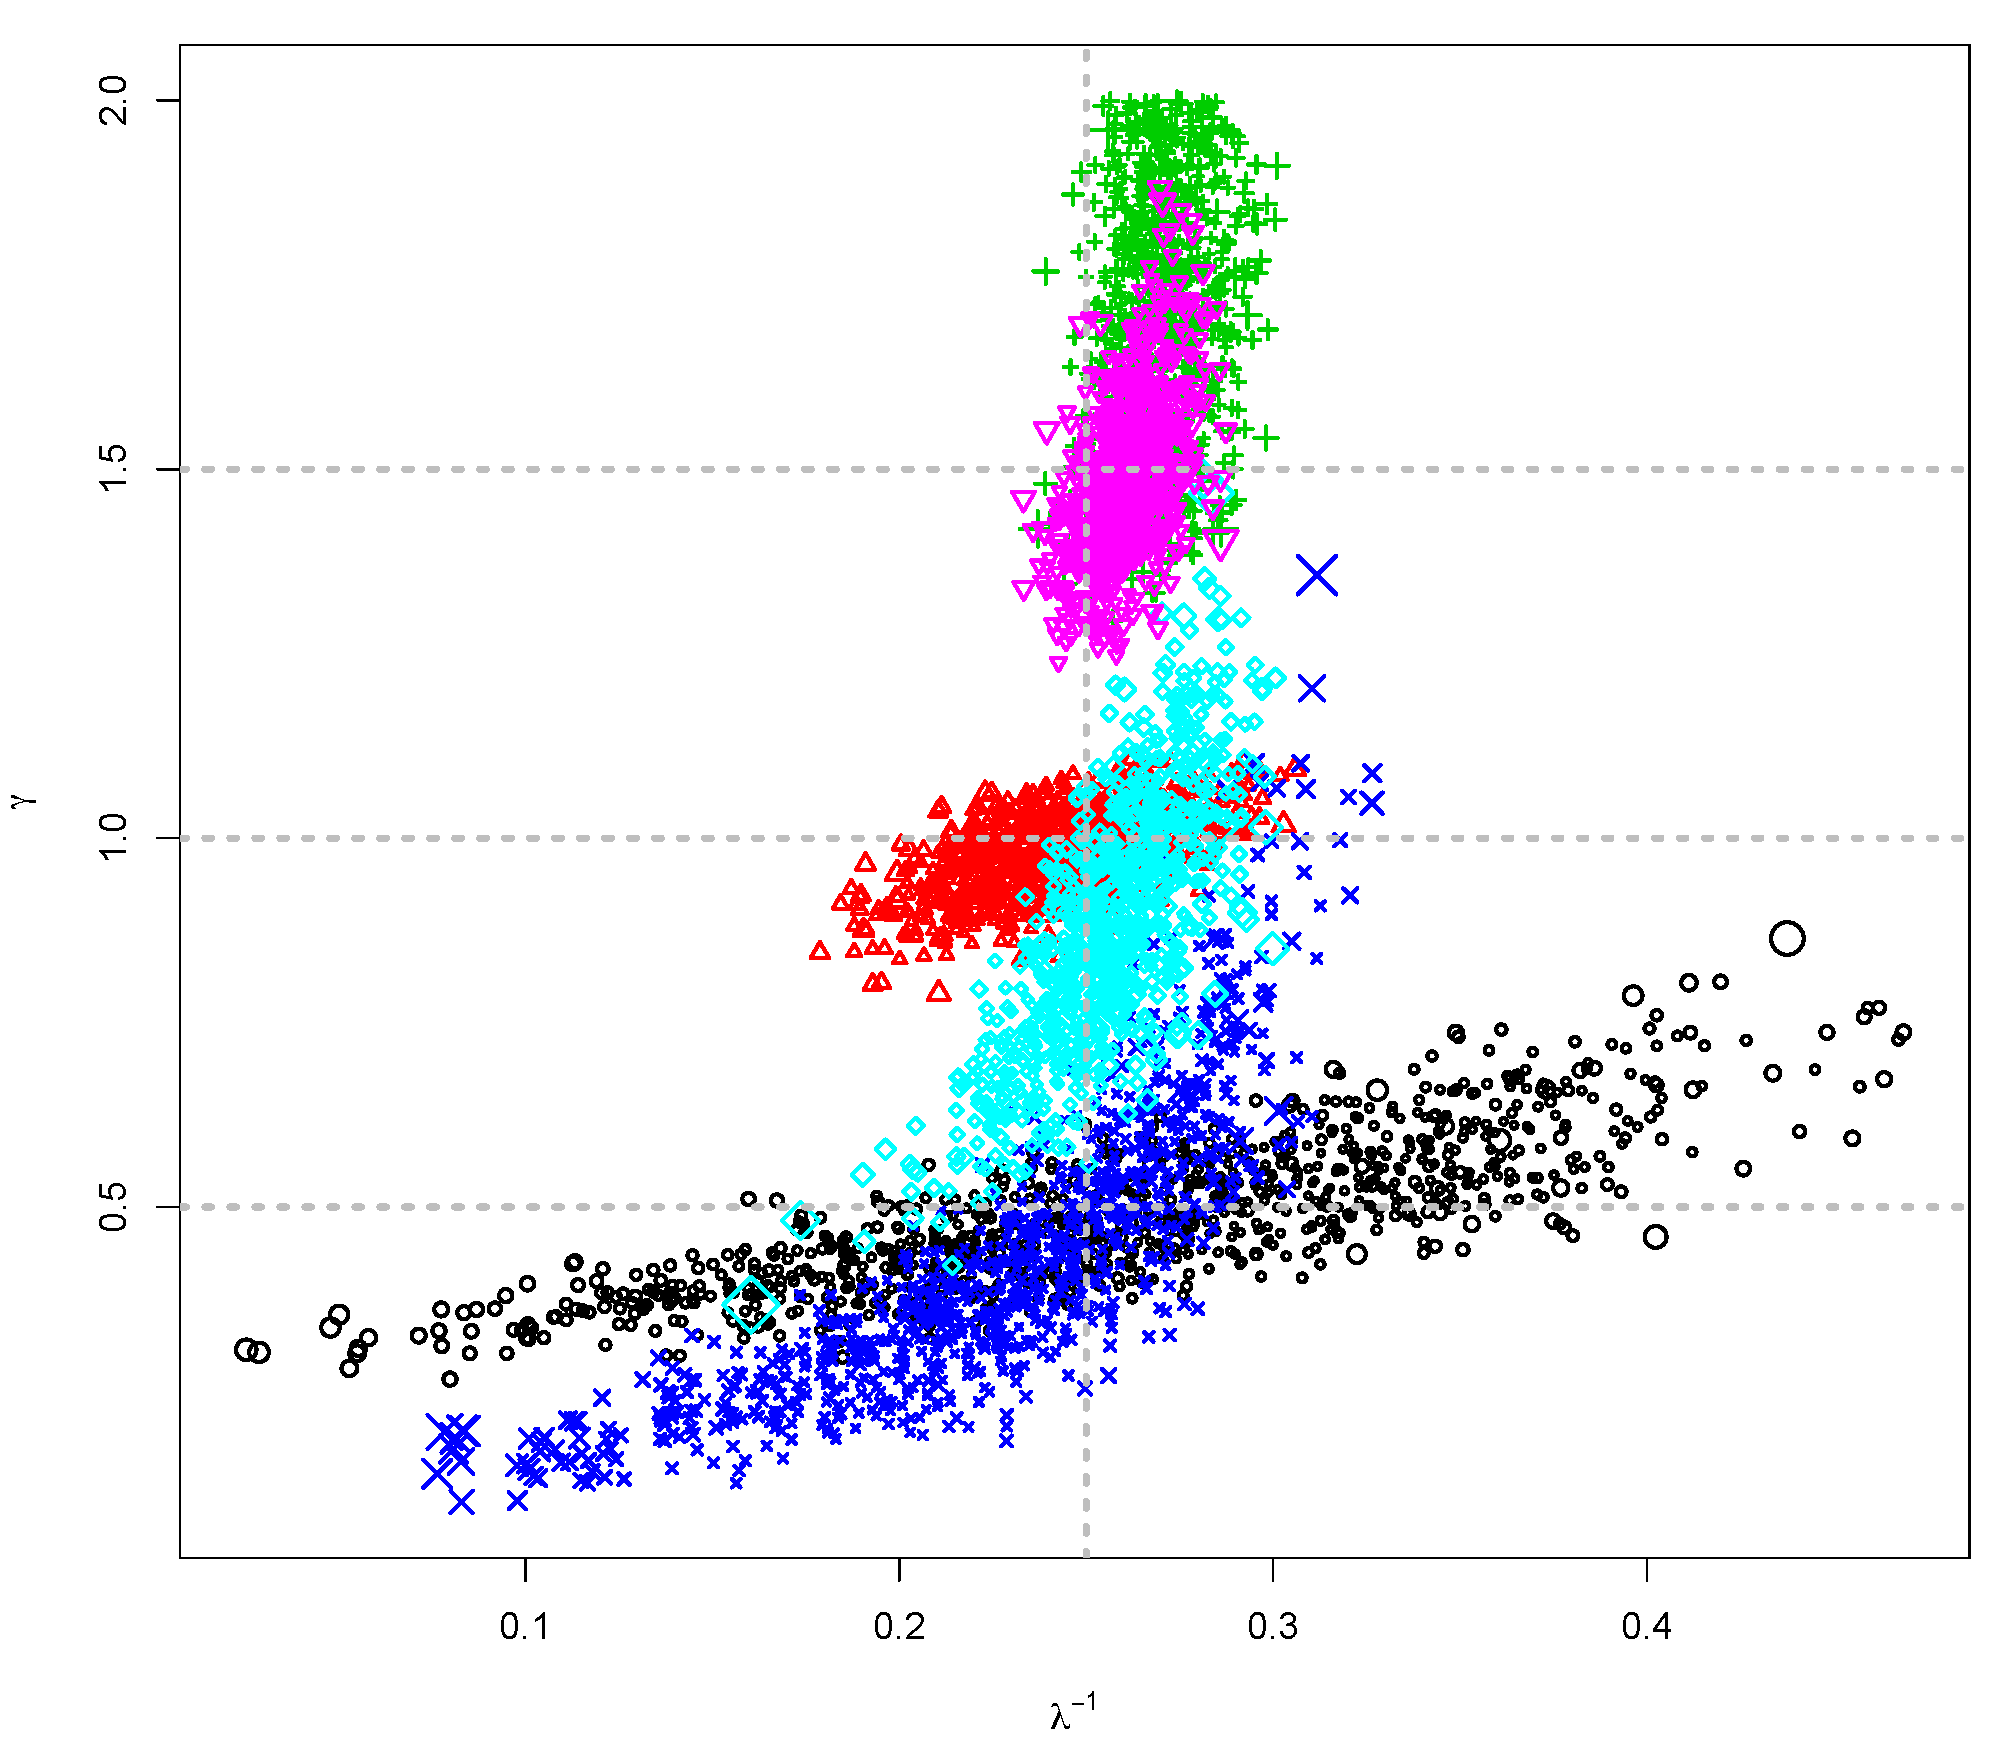
\includegraphics[width = \textwidth]{figures/joint_k_gamma.pdf} 
\caption{ABC Joint $(\lambda^{-1}, \gamma)$}\label{subfig:joint_gamma_k}
\end{subfigure}
\begin{subfigure}{0.32\textwidth}
\centering
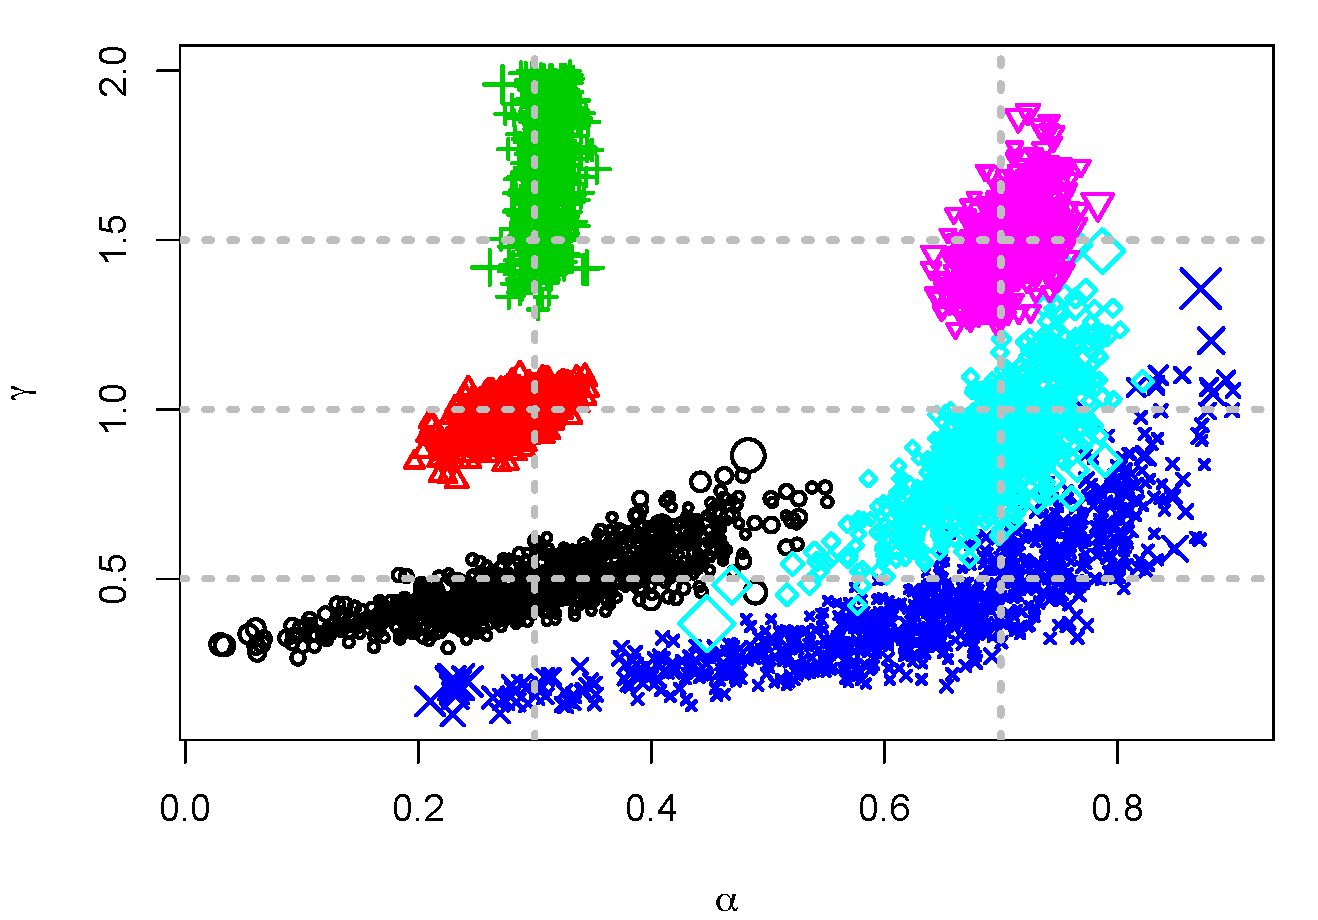
\includegraphics[width = \textwidth]{figures/joint_alpha_gamma.pdf} 
\caption{ABC Joint $(\alpha, \gamma)$}\label{subfig:joint_gamma_alpha}
\end{subfigure} \\
\caption{Pairwise ABC posterior particles samples of (a) $(\lambda^{-1}, \alpha)$, (b) $(\lambda^{-1}, \gamma)$, and (c) $(\alpha, \gamma)$ for the simulation settings of Table~\ref{tab:sim_study}.  The different color and types of points indicate the input parameter values, and the size of the plot symbol is scaled with the particle weight.
}
\label{fig:abc_pa_joints}
\end{figure}




\begin{figure}[htbp]
   \centering
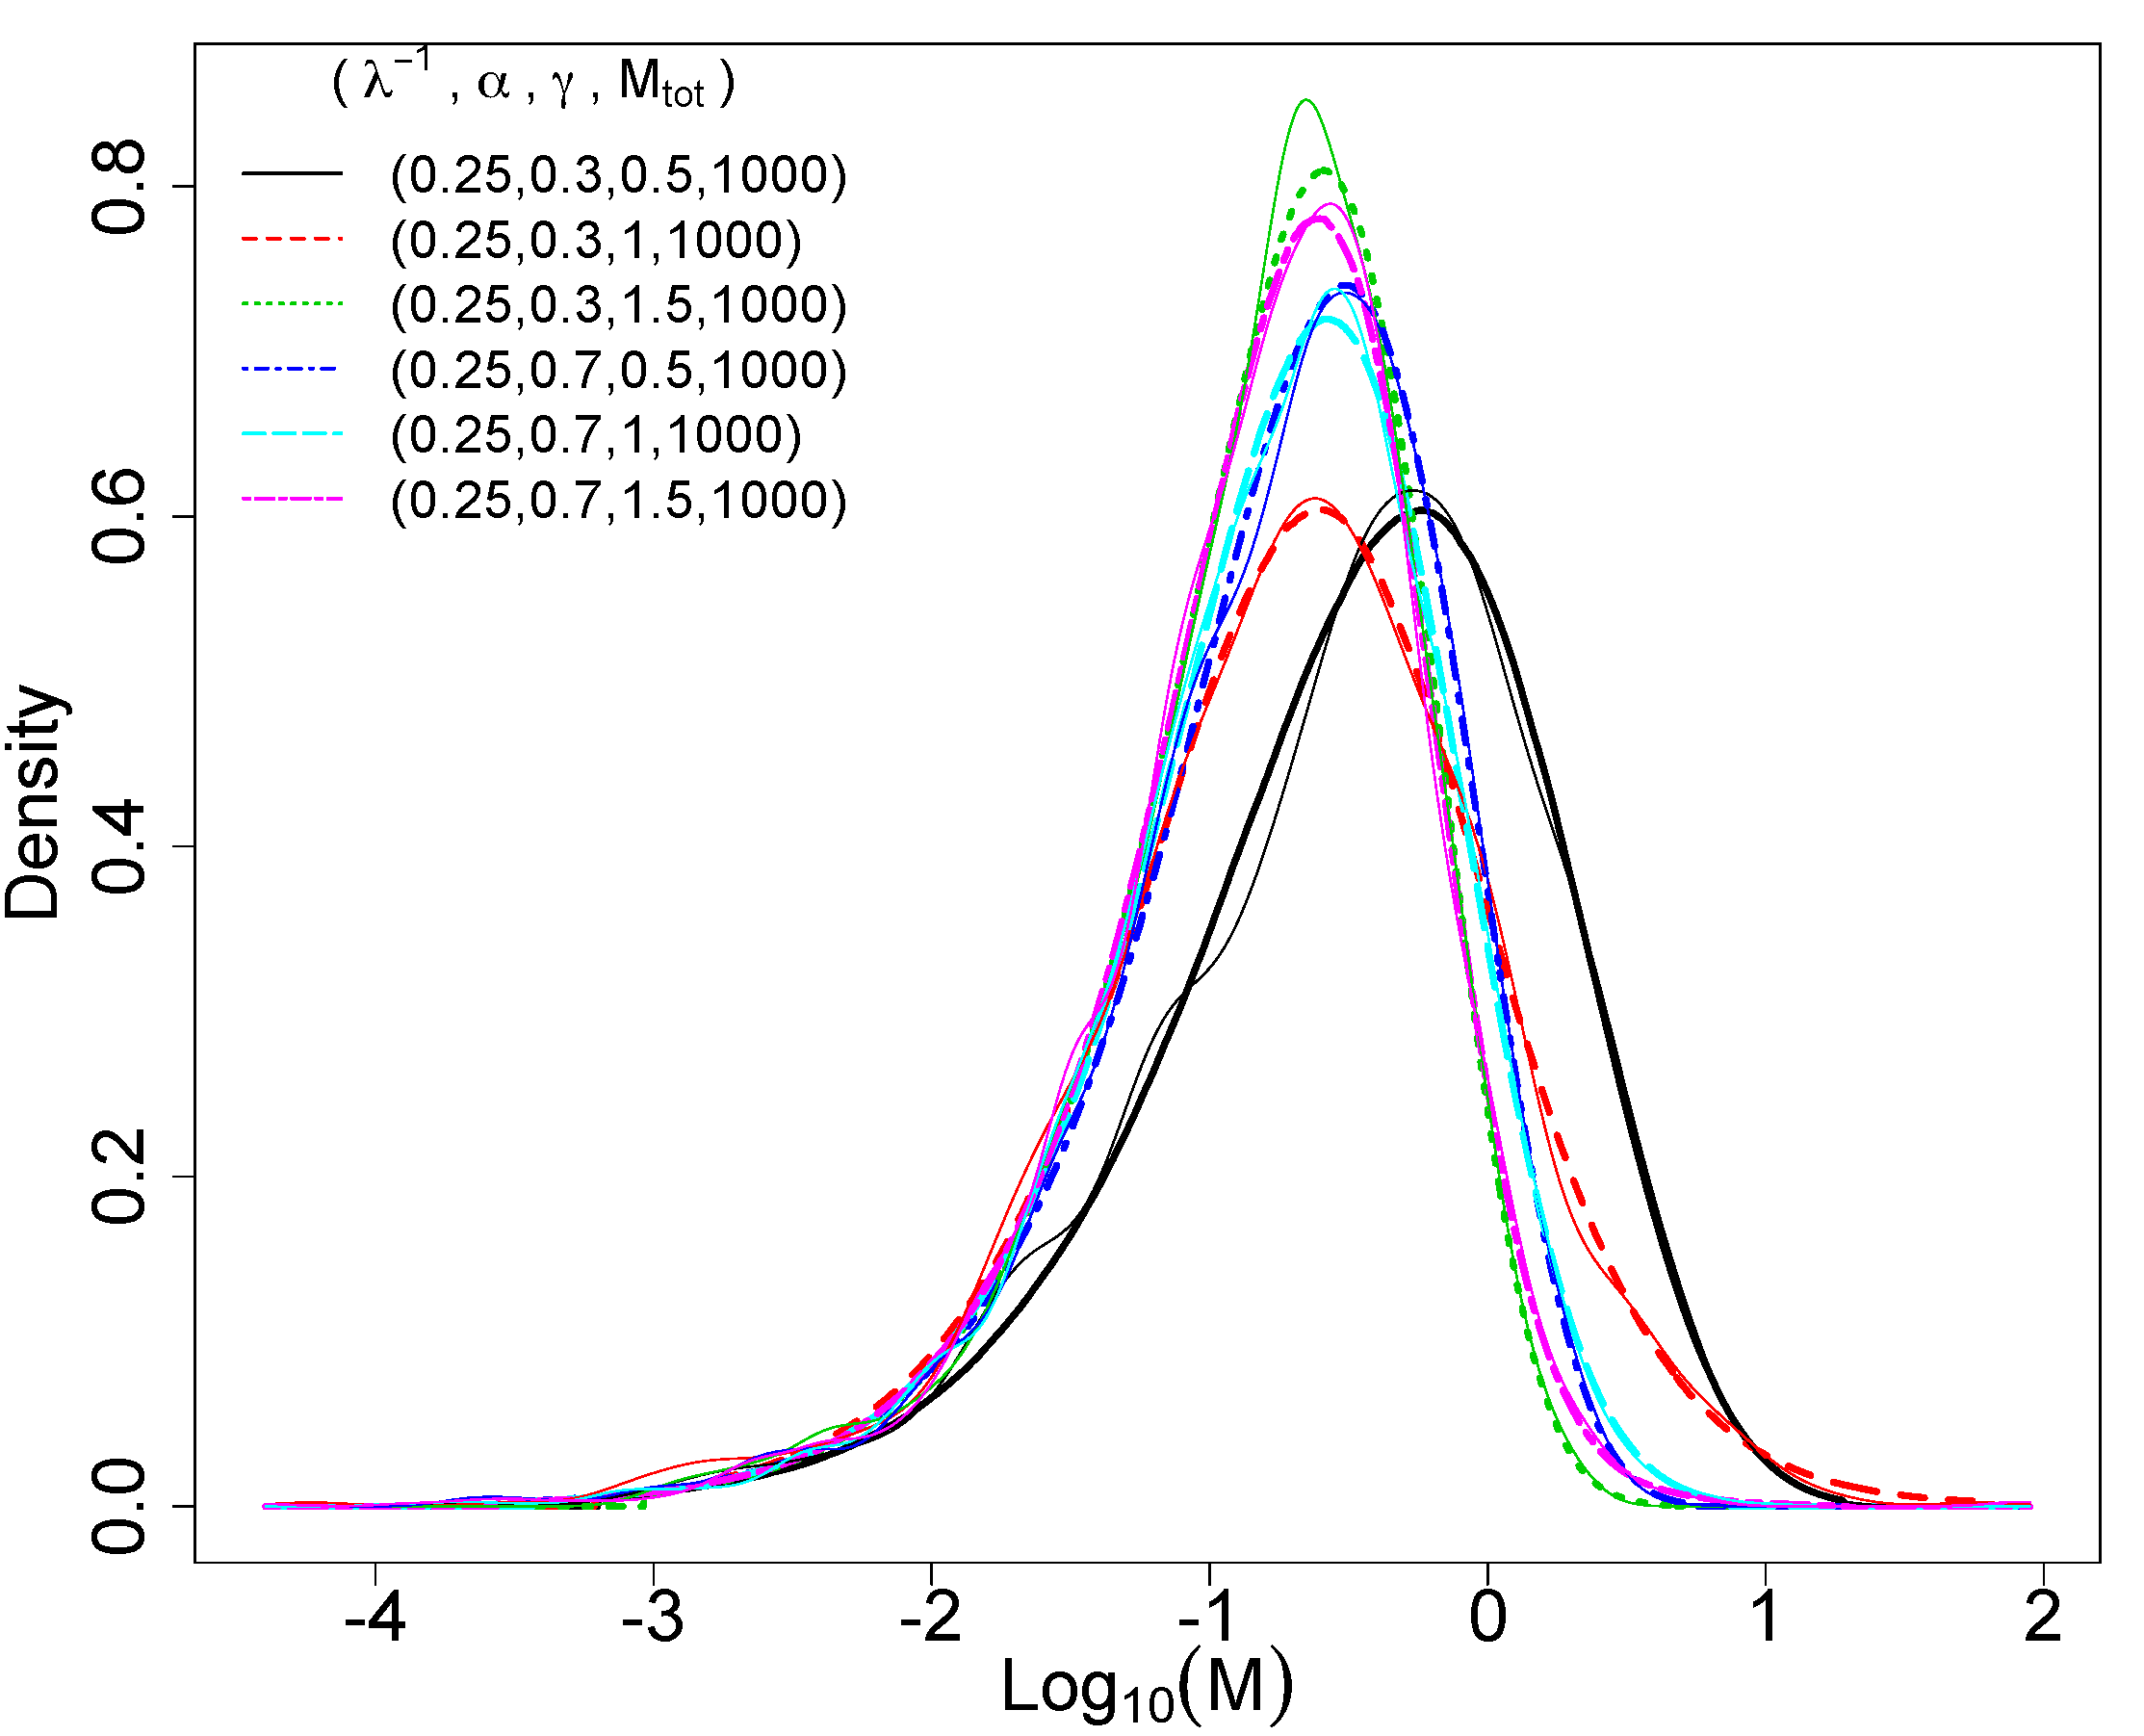
\includegraphics[width = .75\textwidth]{figures/sim_study_imf_combined.pdf} 
   \caption{ABC posterior predictive IMFs for the simulation settings of Table~\ref{tab:sim_study}.  The different color and line types indicate the median ABC posterior predictive IMF for the various input parameter values combinations, $(\lambda^{-1}, \alpha, \gamma, \Mtot)$; the thin solid lines of different colors display the observed IMF associated with the input parameter value combination with the matching color (see Figure~\ref{fig:true_imf}).
The posterior predictive IMFs were derived from taking 1000 draws from the final ABC posteriors in each setting, and then simulating an IMF using the sampled values. 
   }
%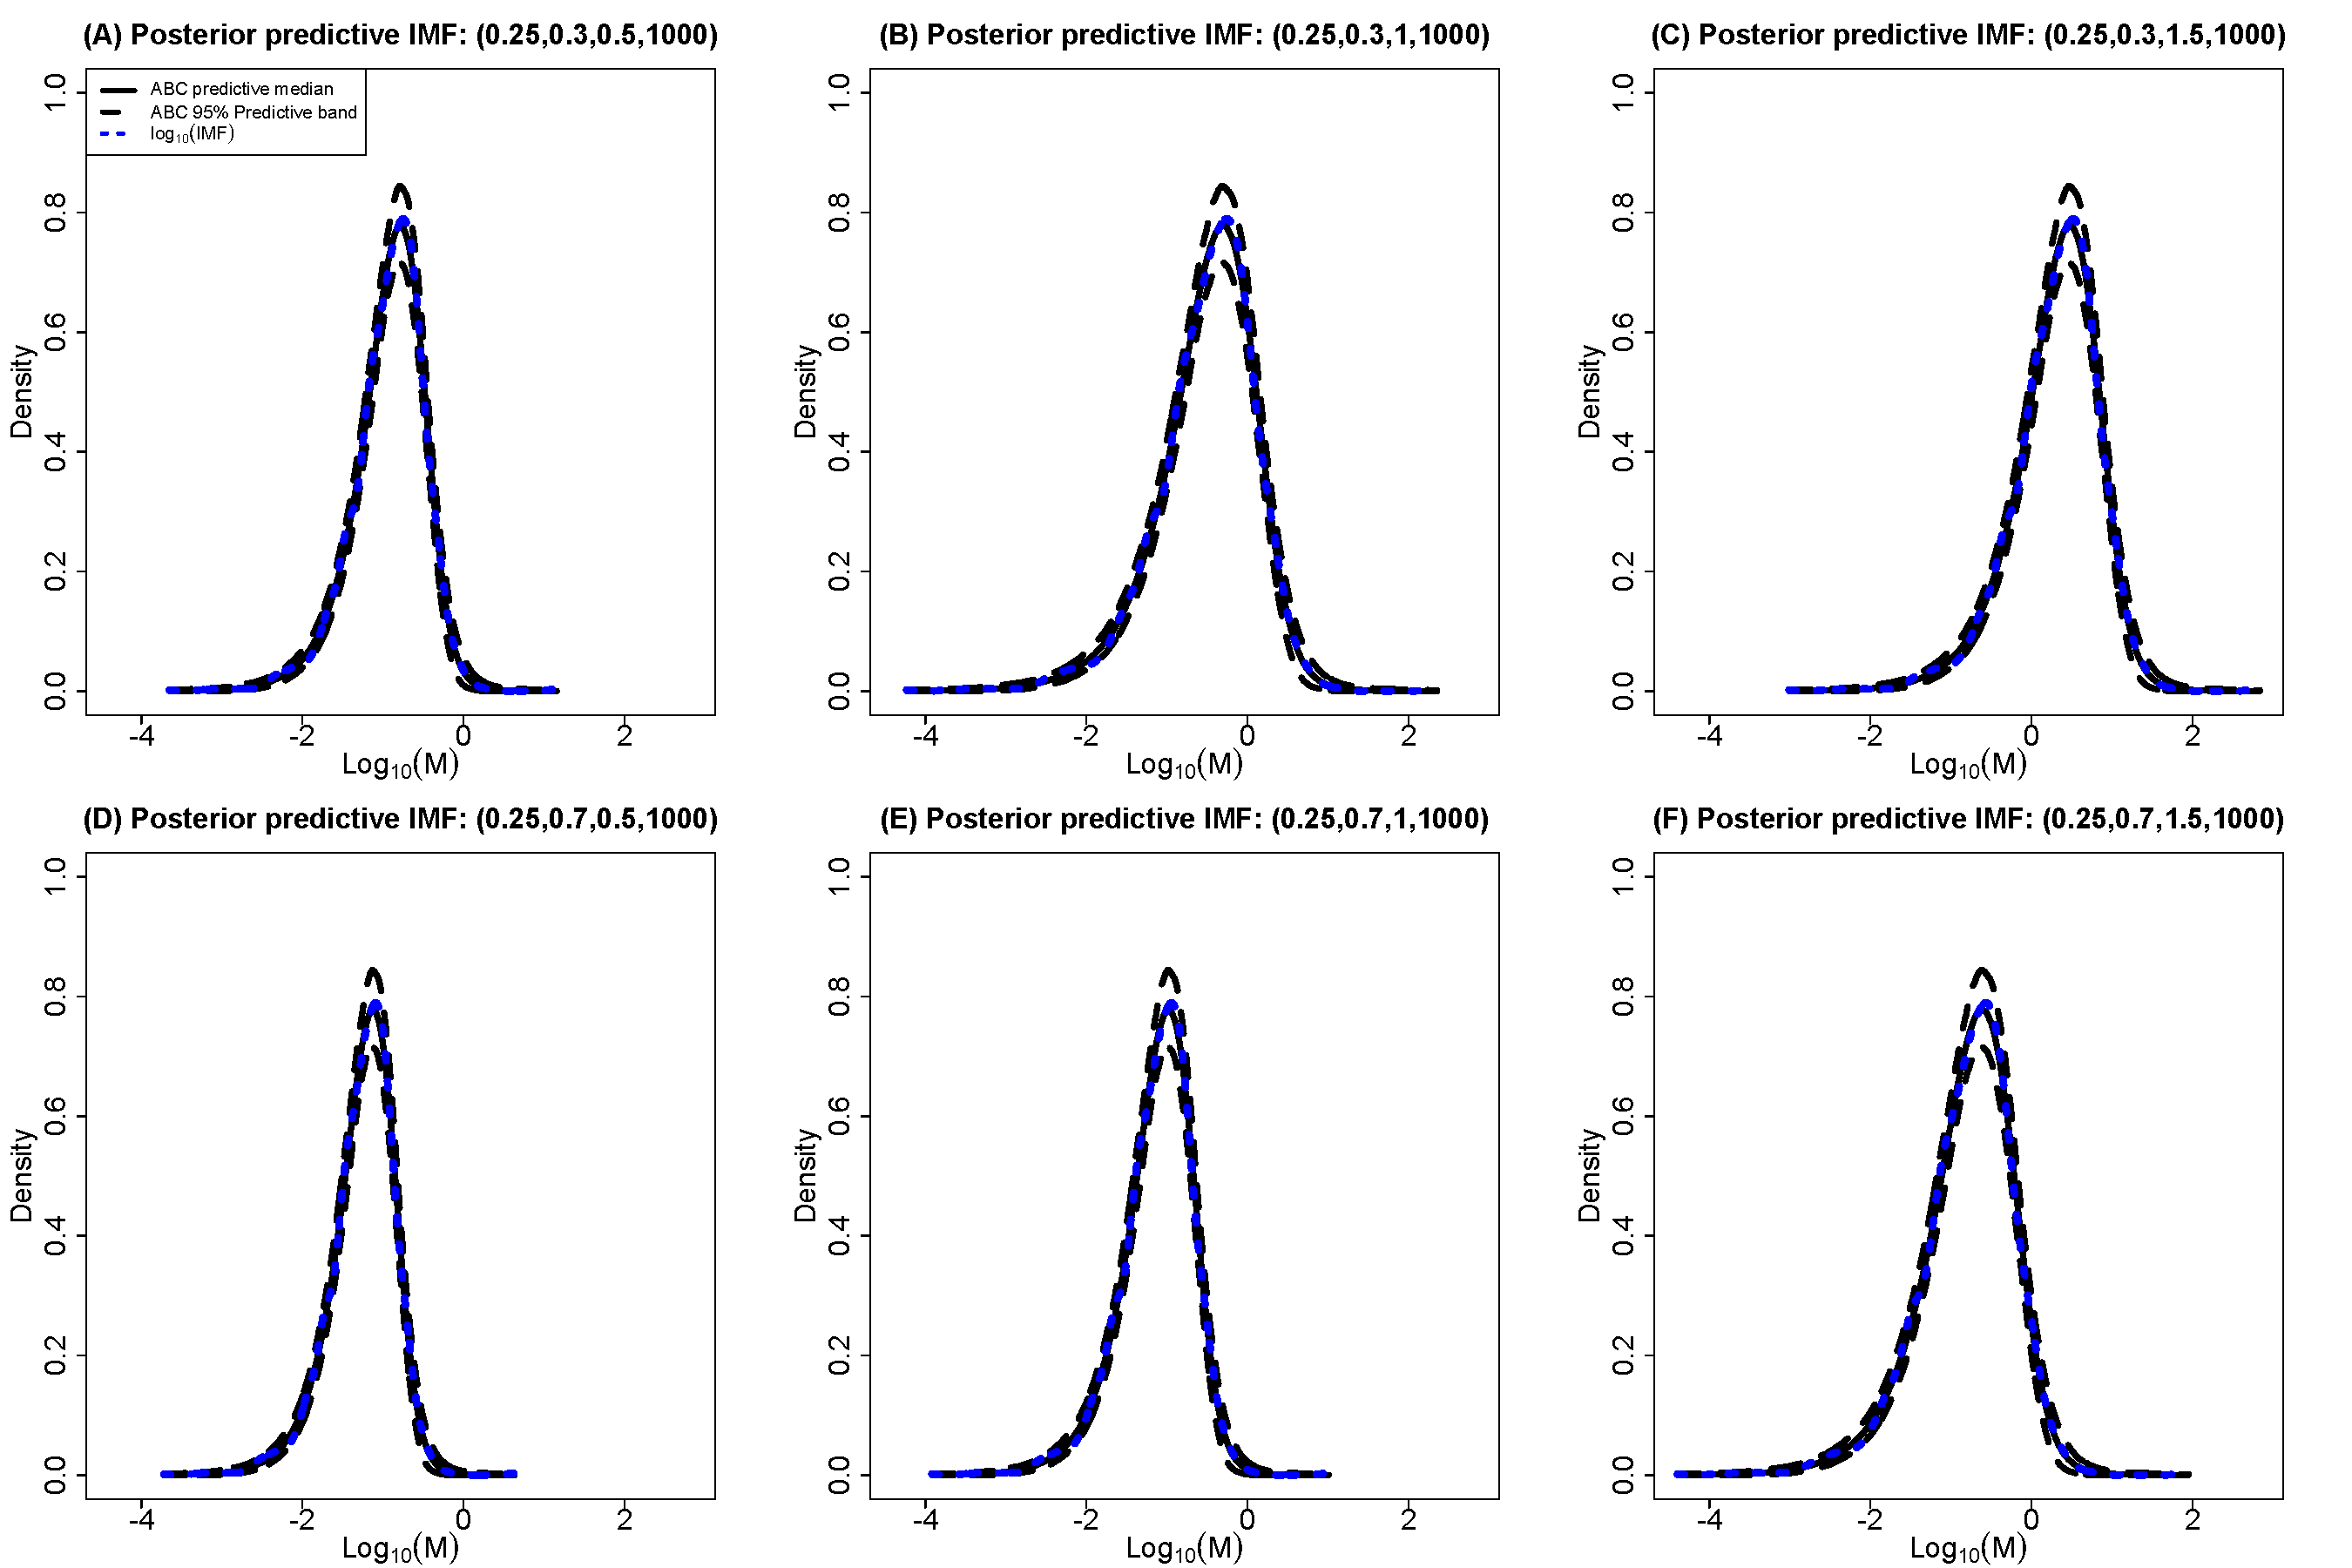
\includegraphics[width = .5\textwidth]{figures/sim_study_imf.pdf} 
%   \caption{ABC posterior predictive IMFs for the simulation settings of Table~\ref{tab:sim_study}.  The blue dotted lines display the true IMF used in each simulation setting, the solid black line is the median ABC posterior predictive IMF, and the dashed black lines indicate a point-wise 95\% credible band.  The posterior predictive IMFs and band were derived from taking 1000 draws from the final ABC posteriors in each setting, and then simulating an IMF using the sampled values.  The input parameter values, $(\lambda^{-1}, \alpha, \gamma, \Mtot)$, are displayed in each sub-plot title.
%   }
   \label{fig:abc_pa_imf}
\end{figure}

\subsubsection{Simulated data with observational effects}

\jessi{running more simulations for this section}

%
%\begin{figure}[htbp]
%\begin{subfigure}{0.32\textwidth}
%\centering
%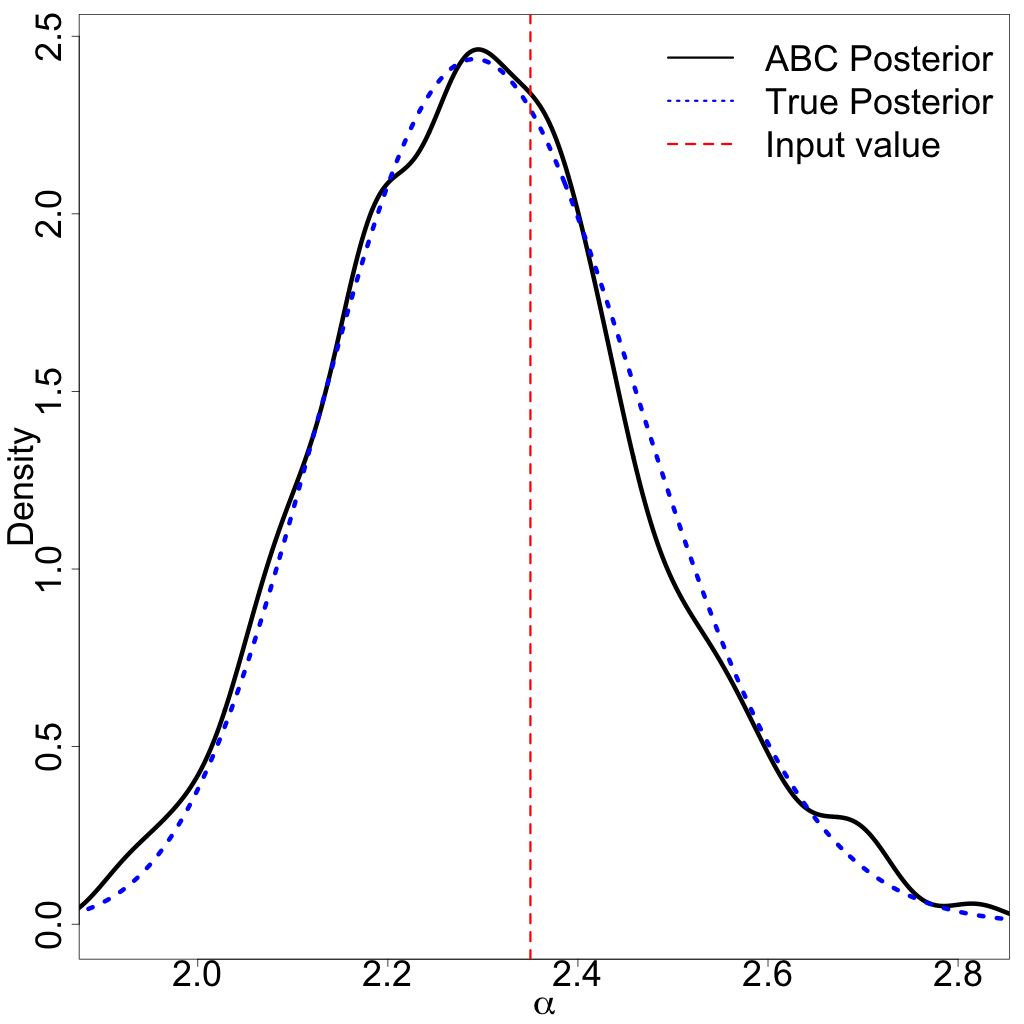
\includegraphics[width=\textwidth]{figures/basic_1_1000_alpha.png}
%\caption{Posterior for $\alpha$}\label{subfig:basic_alpha}
%\end{subfigure}
%\begin{subfigure}{0.32\textwidth}
%\centering
%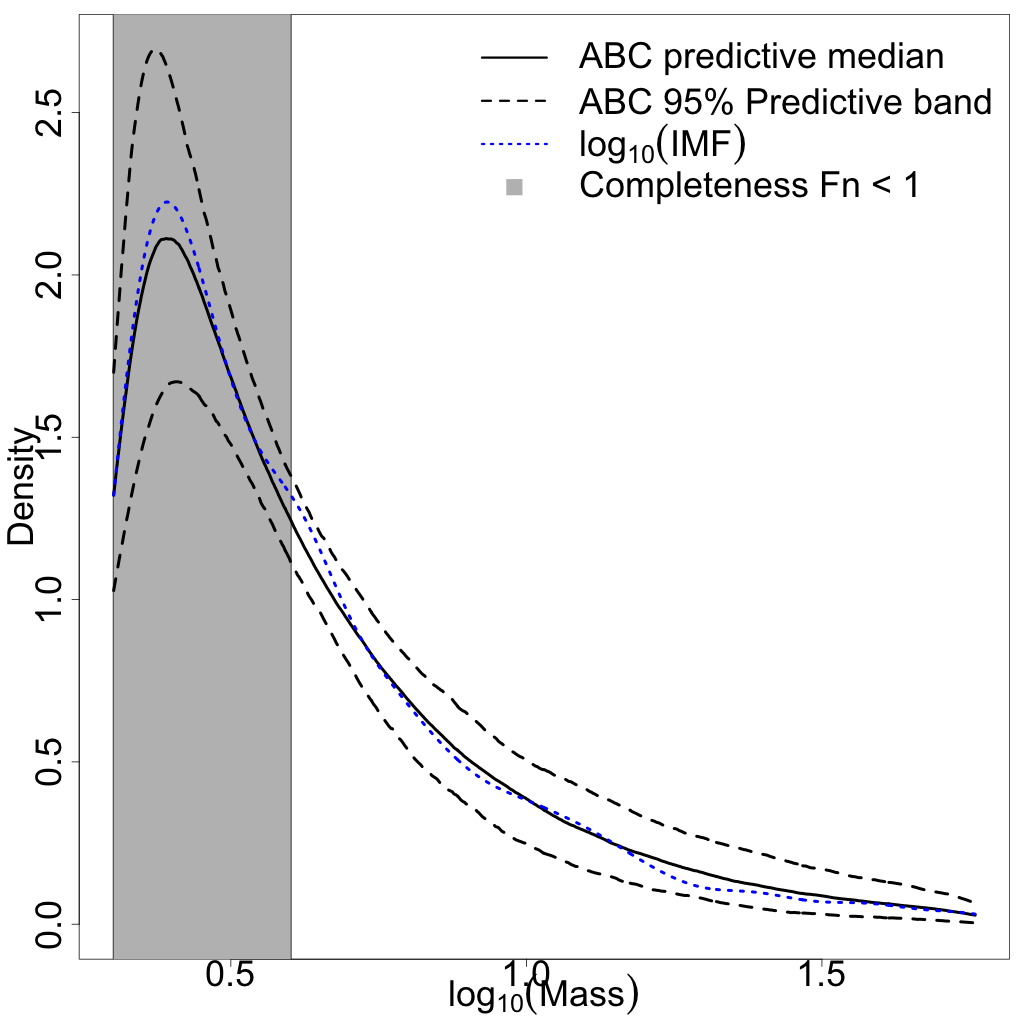
\includegraphics[width=\textwidth]{figures/basic_1_1000_predictive_imf.png}
%\caption{Posterior predictive IMF}\label{subfig:basic_imf}
%\end{subfigure}
%\begin{subfigure}{0.32\textwidth}
%\centering
%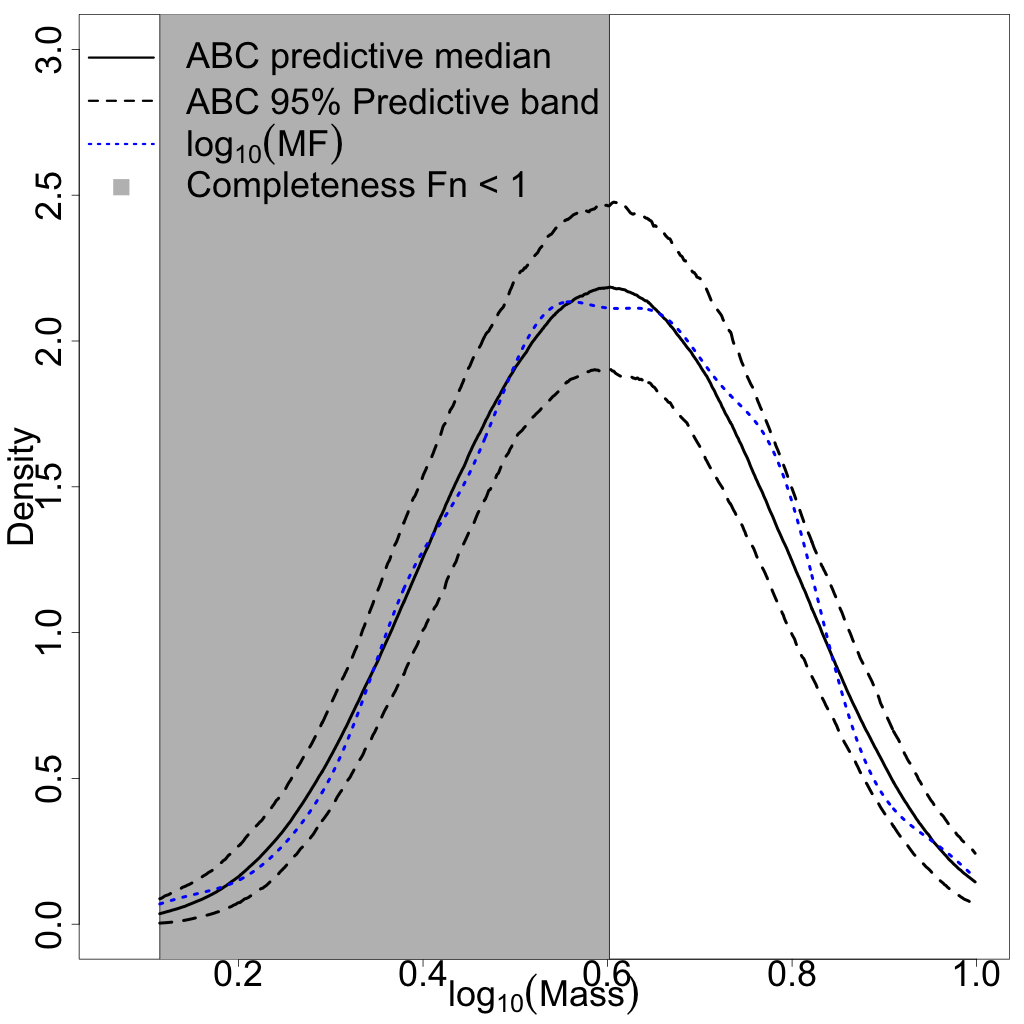
\includegraphics[width=\textwidth]{figures/basic_1_1000_predictive_mf.png}
%\caption{Posterior predictive MF}\label{subfig:basic_mf}
%\end{subfigure}        
%   \caption{Results from stimulated data with observational effects applied.  (A) The ABC posterior for $\alpha$ (solid black) compared to the true posterior (dotted blue) of Equation~\eqref{eq:simple_posterior} using an input value of 2.35 (dashed vertical red).  (B) The median of the posterior predictive IMF (solid black) with a corresponding 95\% point-wise predictive band (dashed black) compared to the true IMF (blue dotted) which was simulated dataset before aging, completeness, or uncertainty were applied, and the gray shaded region indicates where the completeness function was less than 1.  (C) The median of the posterior predictive MF (solid black) with a corresponding 95\% point-wise predictive band (dashed black) compared to the observed MF (dotted blue) which was the simulated dataset after aging, completeness, and uncertainty were applied.  For the posterior predictive IMF, 1000 draws were made from the ABC posterior of (A) and then 1000 cluster samples were drawn from the power law simulation model.  For the posterior predictive MF, the 1000 cluster samples used for (B) were then put through the forward model to apply the aging, completeness, and measurement error effects.
%} \label{fig:abc_sim_obs}
%\end{figure}


%----------------------------------------------------------------------------------------------------------------------------------------------
%-----------------------------------------------------------------------------------------------Bate data
%----------------------------------------------------------------------------------------------------------------------------------------------
\section{Astrophysical simulation data}

Next we consider a star cluster generated from a radiation hydrodynamical simulation presented in \cite{Bate2012}.  This simulation results in 183 stars and brown dwarfs formed from a 500 $\Msun$ molecular cloud of uniform density, along with the growth of the stars and brown dwarfs across the duration of the simulation.  Figure~\ref{fig:bate1} displays the growth curves of the 183 objects and the IMF.  The total mass of the resulting objects is about 88.68 $\Msun$.  The details of the simulation can be found in \cite{Bate2012}.  Validation of the simulated cluster was carried out by comparing the simulated cluster with real observations using {\color{red}[ADD CLUSTER COMPARISONS MADE]}. 


marginal ABC posteriors in Figure~\ref{fig:abc_bate_posterior}

Posterior predictive IMF in Figure~\ref{fig:abc_bate_pred}

1000 particles, quantile = 0.25, 5 iterations

final tolerance for MF shape: 0.009360724 

final tolerance for star count:  0.005464481

$\lambda^{-1}$ posterior mean =  0.260

$\alpha$ posterior mean = 0.537

$\gamma$ posterior mean = 1.091



\begin{figure}[htbp]
   \centering
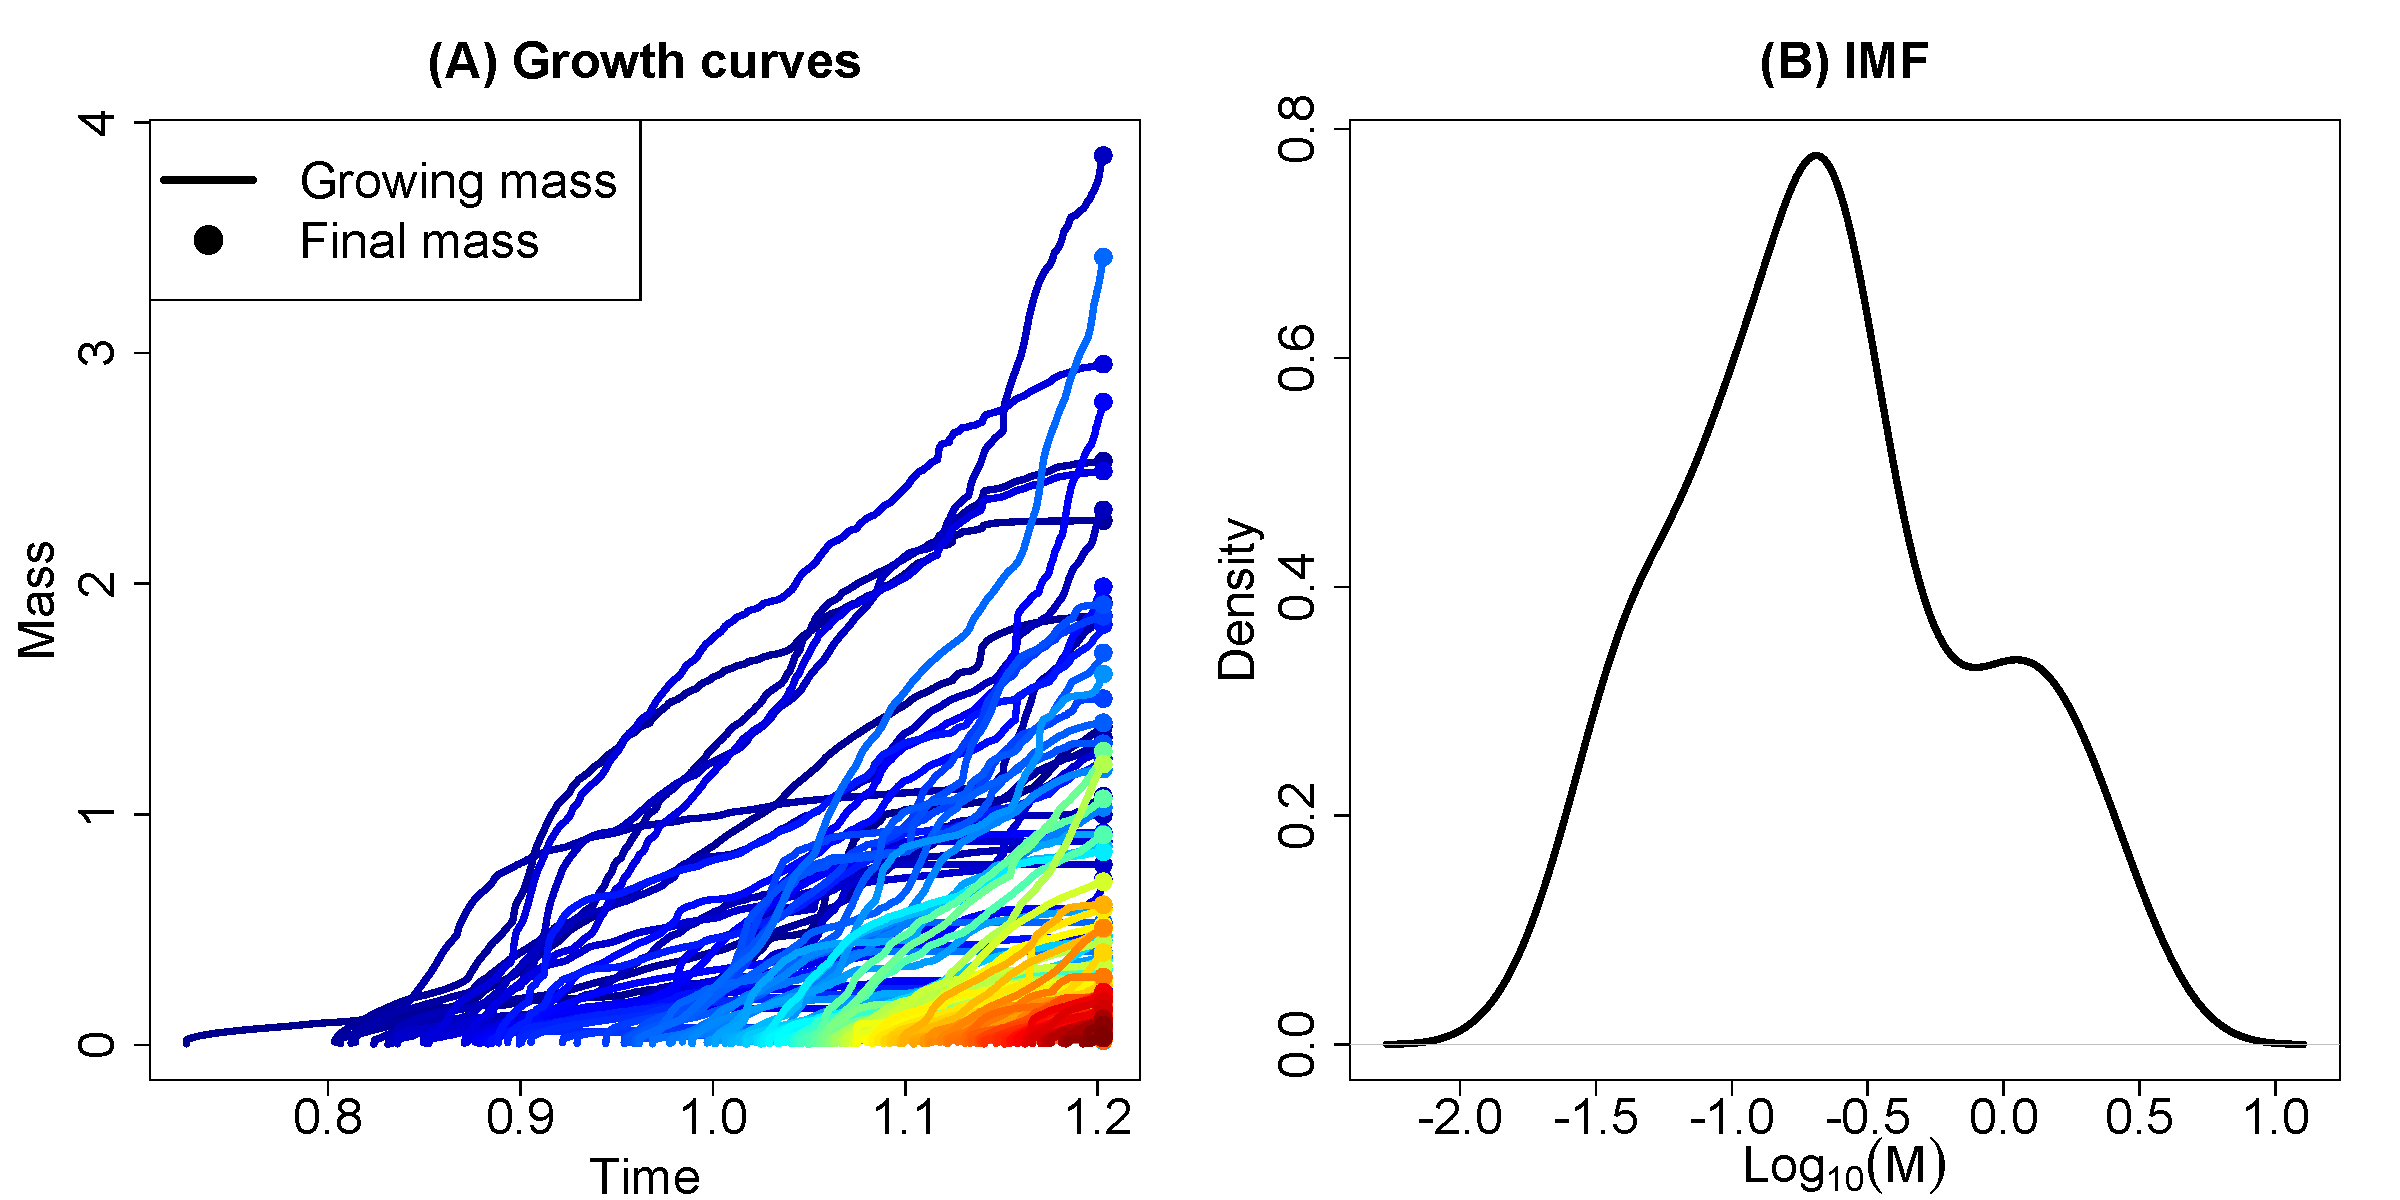
\includegraphics[width = .95\textwidth]{figures/bate_initial.pdf} 
   \caption{Astrophysical simulation data.  (A) The growth of stars and brown dwarfs across simulation time from \cite{Bate2012}, and (B) the resulting IMF.  The colors in (A) distinguish the 183 stars and brown dwarfs.
   }
   \label{fig:bate1}
\end{figure}


\begin{itemize}
\item  Section 2.1 of Bate on sink particles seems to describe the accretion process
\item In Bate - should not have significant super-linear attachment.  Check to see if he has examples where there is super-linear attachment.
\item[] ``Sink particles are permitted to merge in the calculation if they passed within 0.01 au of each other. However, no mergers occurred during the calculation.''
\item 2.3.2 has discussion about the accretion radius
\item  Changes in the number of stars and mean masses with vs. without radiative feedback
\item ``In this paper, we refer to the mass function as an �IMF� because we compare it to the observed IMF since the PMF cannot yet be determined observationally. How- ever, it should be noted that how a PMF transforms into the IMF depends on the accretion history of the protostars and how the star formation process is terminated.''
\end{itemize}

\begin{figure}[htbp]
\begin{subfigure}{0.32\textwidth}
\centering
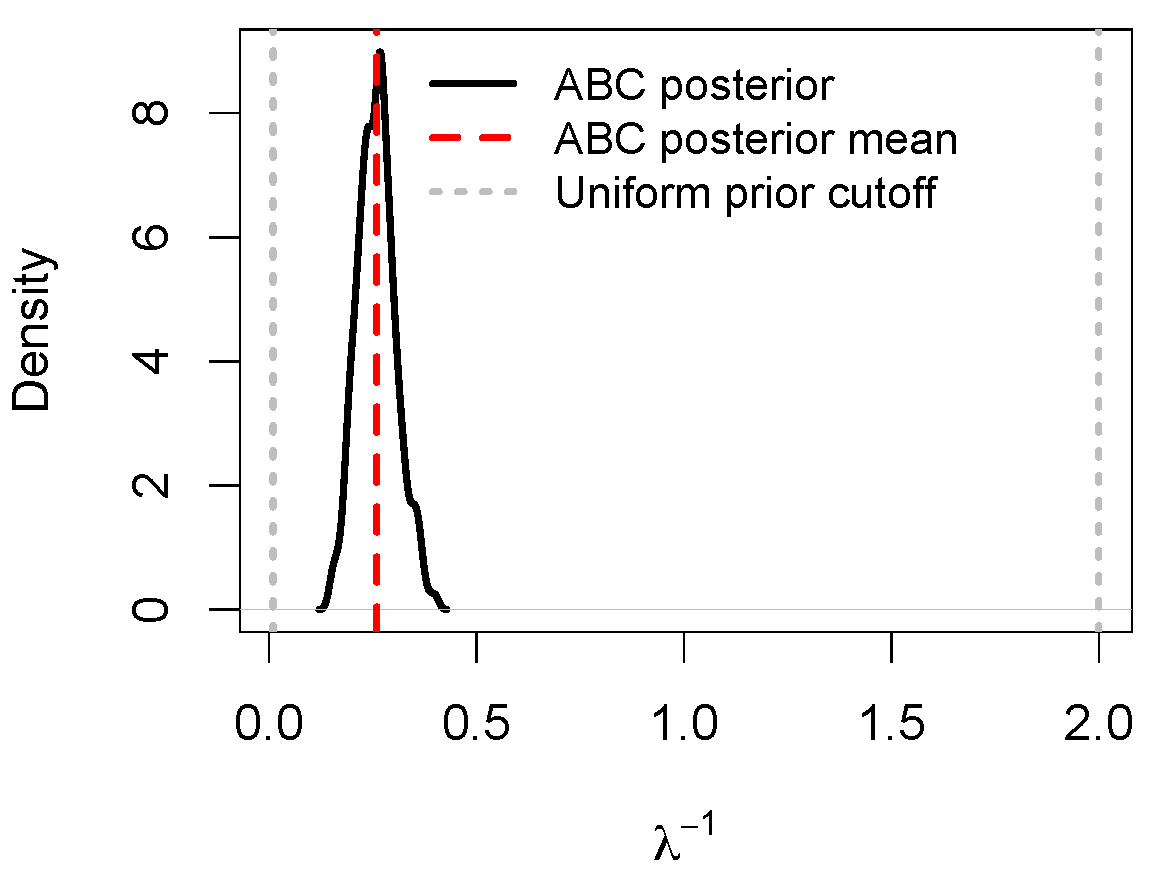
\includegraphics[width = .95\textwidth]{figures/bate_marginal_k.pdf} 
\caption{ABC posterior for $\lambda^{-1}$}\label{subfig:bate_k}
\end{subfigure}
\begin{subfigure}{0.32\textwidth}
\centering
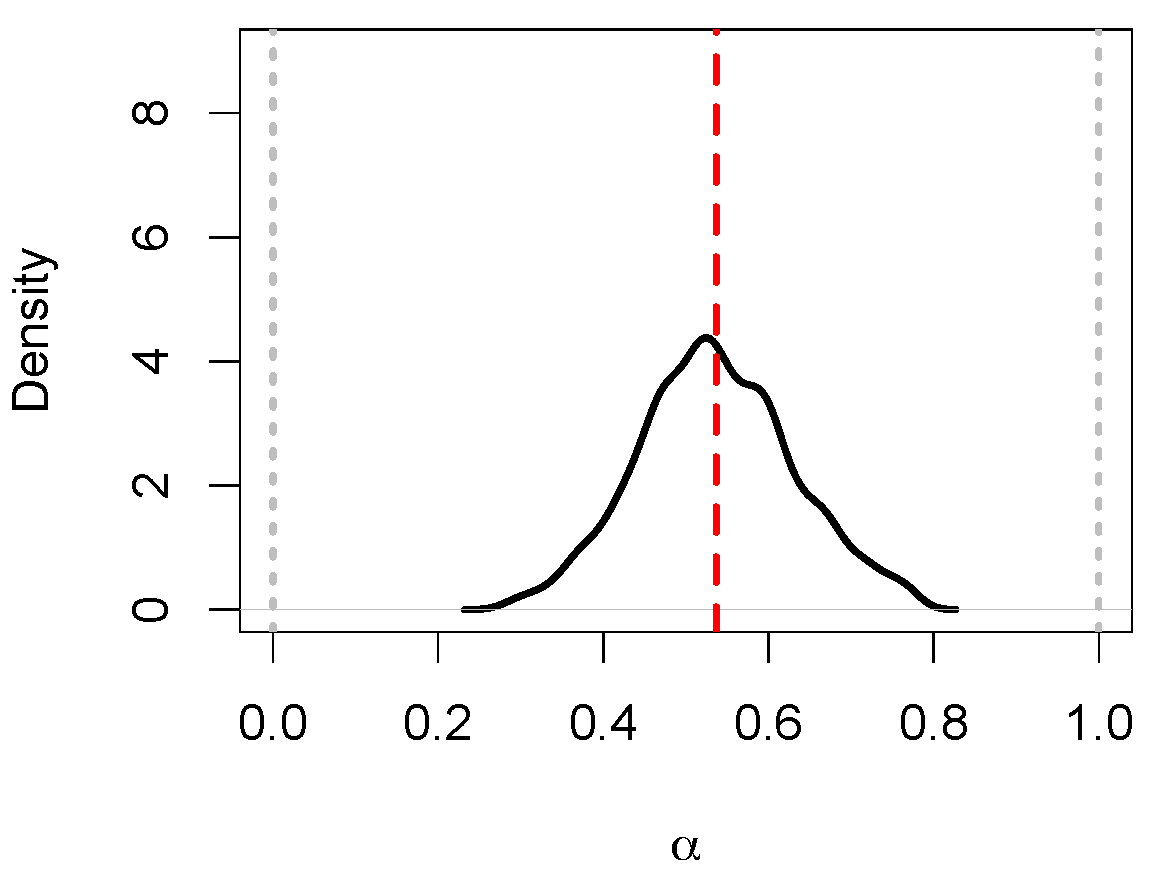
\includegraphics[width = .95\textwidth]{figures/bate_marginal_alpha.pdf} 
\caption{ABC posterior for $\alpha$}\label{subfig:bate_alpha}
\end{subfigure}
\begin{subfigure}{0.32\textwidth}
\centering
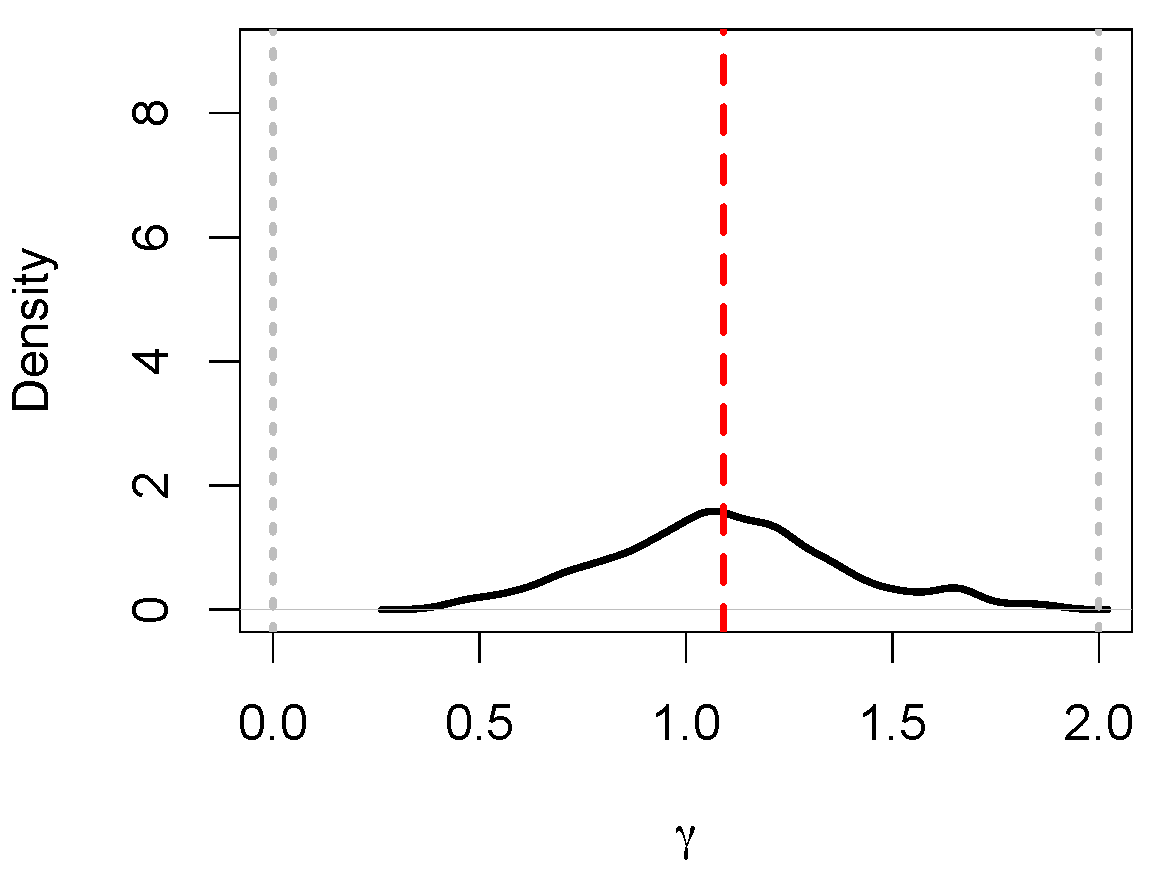
\includegraphics[width = .95\textwidth]{figures/bate_marginal_gamma.pdf} 
\caption{ABC posterior for $\gamma$}\label{subfig:bate_gamma}
\end{subfigure}
\caption{Marginal ABC posteriors for astrophysical simulation data from \cite{Bate2012}.  The vertical dashed red lines indicate the ABC posterior mean, and the dotted gray lines indicate the range of the uniform prior for the parameter.  
 }
   \label{fig:abc_bate_posterior}
\end{figure}





\begin{figure}[htbp]
\centering
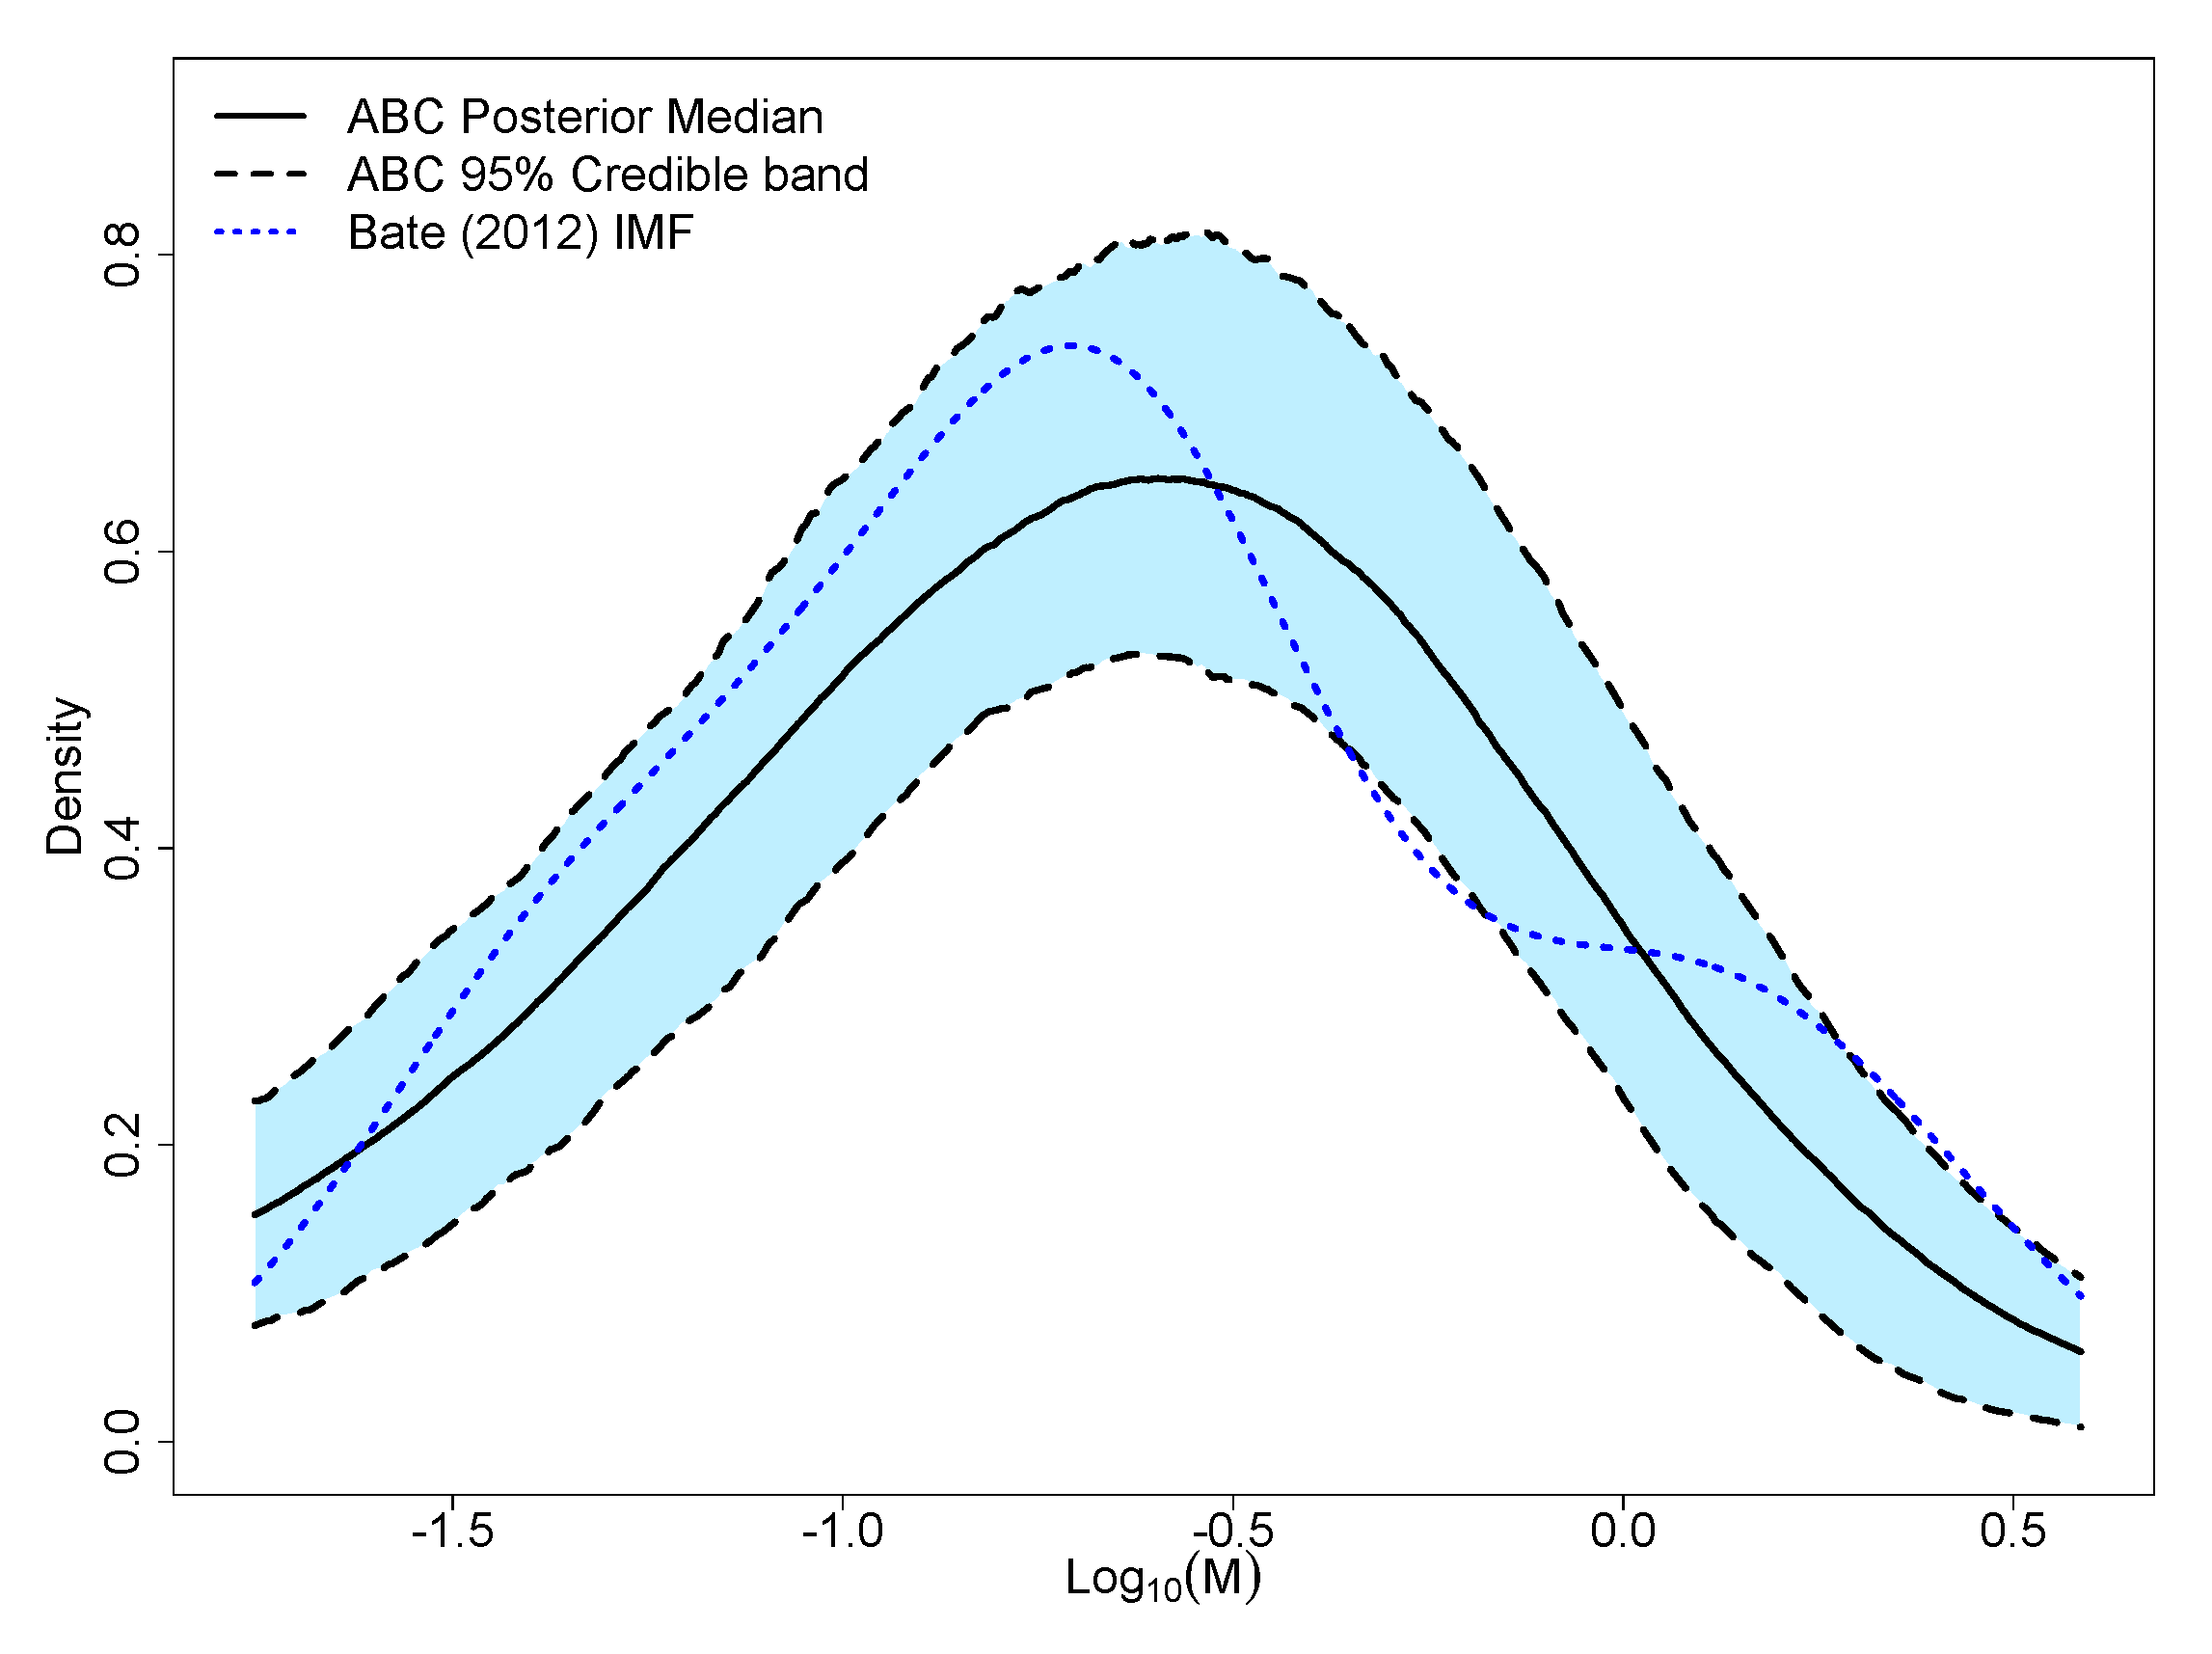
\includegraphics[width=.75\textwidth]{figures/bate_pred_imf.pdf}
 \caption{Posterior predictive IMF for astrophysical simulation data from \cite{Bate2012}. 
The median of the posterior predictive IMF (solid black) with a corresponding 95\% point-wise predictive band (dashed black) compared to the true IMF (blue dotted).  For the posterior predictive IMF, 1000 draws were made from the ABC posteriors of Figure~\ref{fig:abc_bate_posterior} and then 1000 cluster samples were drawn from the proposed forward model.  
} \label{fig:abc_bate_pred}
\end{figure}


%----------------------------------------------------------------------------------------------------------------------------------------------
%-----------------------------------------------------------------------------------------------Discussion
%----------------------------------------------------------------------------------------------------------------------------------------------
\section{Discussion}
\label{discussionSec}

Accounting for complex dependencies in observations, such as the initial masses of stars forming from a molecular cloud, is a challenging statistical problem.  A possible, but unsatisfactory, resolution is simply to proceed as though the dependency is weak enough to assume independence.  Instead, we draw from ideas in the preferential attachment literature proposing a new forward model to be used in an ABC algorithm.  
Though the new generative model was motivated by inference on stellar IMFs, it is generalizable to other applications that operate on a similar principle of dependent data.
First we verified that the ABC approach works under the simplifying assumption of independence to ensure the true posterior was recoverable using ABC with the various observational effects.  Then we introduced the new generative model, which starts with the total mass and stochastically builds individuals stars of particular mass.  The new model is general in the sense that it captures the dependencies among the masses of the stars, and also can accommodate standard models proposed in the astronomical literature.

The ONC is an interesting object of study among astronomers. 
The proposed preferential attachment model fitted via ABC captures the fluctuations in the observed mass function, as well as accounting for varying uncertainty as a function of available data in different regions of the mass range.  
While the proposed model is able to account for the dependency among the masses (along with the aging, completeness function, and observation uncertainty effects), it would be scientifically and statistically interesting to generalize the generative model to capture the spatial dependency among the observations.  
Intuitively, such an approach could account for a mechanism that limits the formation of multiple very massive stars relatively near to each other.  
Understanding the spatial distribution of masses of stars during formation would help advance our understanding stellar formation and evolution.  
Additionally, we did not attempt to capture the possible disturbances to the observed mass function as stars die, with the exception of deaths of the most massive stars.  

Overall, the proposed generative model and ABC methodology provide a useful framework for dealing with complex physical processes that are otherwise difficult to work with in a statistically rigorous fashion.
As increasing computational resources allow for greater model complexity in studies of astronomy and other scientific fields, the proposed and other ABC algorithms may open new opportunities for Bayesian inference in challenging problems. 

%%----------------------------------------------------------------------------------------------------------------------------------------------
%%-----------------------------------------------------------------------------------------------Appendix
%%----------------------------------------------------------------------------------------------------------------------------------------------
\appendix
\section{ABC summary statistic selection} \label{app:summary}
In order to select effective summary statistics for the proposed model, we first employ the ABC methodology in a simplified study that focuses on the posterior of the power law parameter $\alpha$ from Equation~\eqref{eq:imf}.  We generate a cluster of $n = 10^3$ stars from an IMF with slope $\alpha = 2.35$  \citep{salpeter55}, $\Mmin = 2$, and $\Mmax = 60$,  a uniform prior distribution for $\alpha \in (0, 6)$, and with $\Mmax$ considered known.  This simple model was used in order to check the method against the true posterior of $\alpha$ after the observational and aging effects have been incorporated into the forward model.  We use the bivariate summary statistic and distance function of Equation~\eqref{eq:2da}.  Defining the two-dimensional tolerance sequence as $(\epsilon_{1t}, \epsilon_{2t})$ where the subscript $t$ indicates the algorithm time step, and  $\epsilon_{11}$ and $\epsilon_{21}$ were selected using an adaptive started discussed in Section~\ref{methodSec} using an initial number of draws of $10\times$N with $N = 10^3$.  The algorithm ran for $T = 5$ time steps.
At steps $t = 2,\ldots,T$, $\epsilon_{1t}$ and $\epsilon_{2t}$ were set equal to the $25th$ percentile of the distances retained at the previous step from their corresponding distance functions.


The pseudo-data were aged 30 Myrs with the measurement error of $\sigma = 0.25$ and observation completeness defined by the linear-ramp function in \eqref{eq:ramp}.  Figure~\ref{fig:abc_simple} displays  the ABC posterior resulting from the ABC algorithm along with the true posterior for $\alpha$.  The ABC posterior matches the true posterior, defined as 
\begin{align}
&\pi_F(\alpha \mid  \mobs, M_{\min}, M_{\max}, \nobs, n_{tot}, T_{age}) \propto  \label{eq:simple_posterior}\\ 
&\left \{\Proba(M>T_{age})+\left(\frac{1-\alpha}{M_{\max}^{1-\alpha}-M_{\min}^{1-\alpha}}\right)\int_2^4 M^{-\alpha}\left(1-\frac{M-2}{2}\right )dM\right \}^{n_{tot}-\nobs}  \nonumber \\ \nonumber
& \times \prod_{i=1}^{\nobs}\left\{ \int_2^{T_{age}}(2\pi\sigma^2)^{-\frac{1}{2}}m_i^{-1}e^{-\frac{1}{2\sigma^2}(\log(m_i)-\log(M))^2} \left(\frac{1-\alpha}{M_{\max}^{1-\alpha}-M_{\min}^{1-\alpha}}\right)M^{-\alpha} \right.\\ \nonumber
& \times  \left.\left(I\{M>4\}+\left(\frac{M-2}{2}\right)I\{2\leq M\leq 4\}\right) dM \right\} 
\end{align}
where $T_{age} = \tau^{-1/3} \times 10^{4/3}$ is the upper-tail mass cutoff due to aging.



\begin{figure}[htbp]
\centering
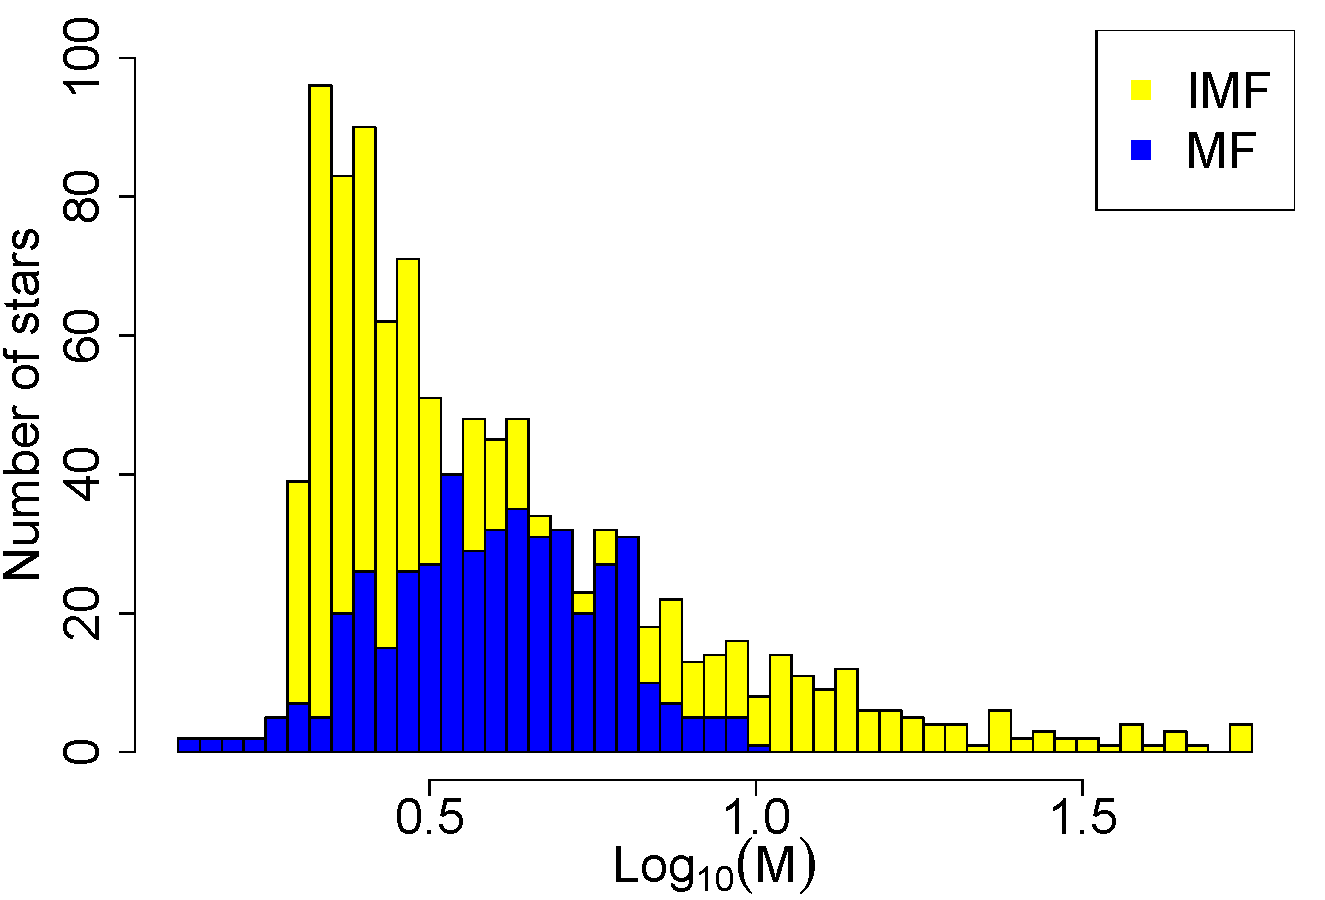
\includegraphics[width=.75\textwidth]{figures/sim_basic_imf_mf_log10.pdf}       
\caption{TBD
} \label{fig:abc_simple_data}
\end{figure}





\begin{figure}[htbp]
\begin{subfigure}{0.32\textwidth}
\centering
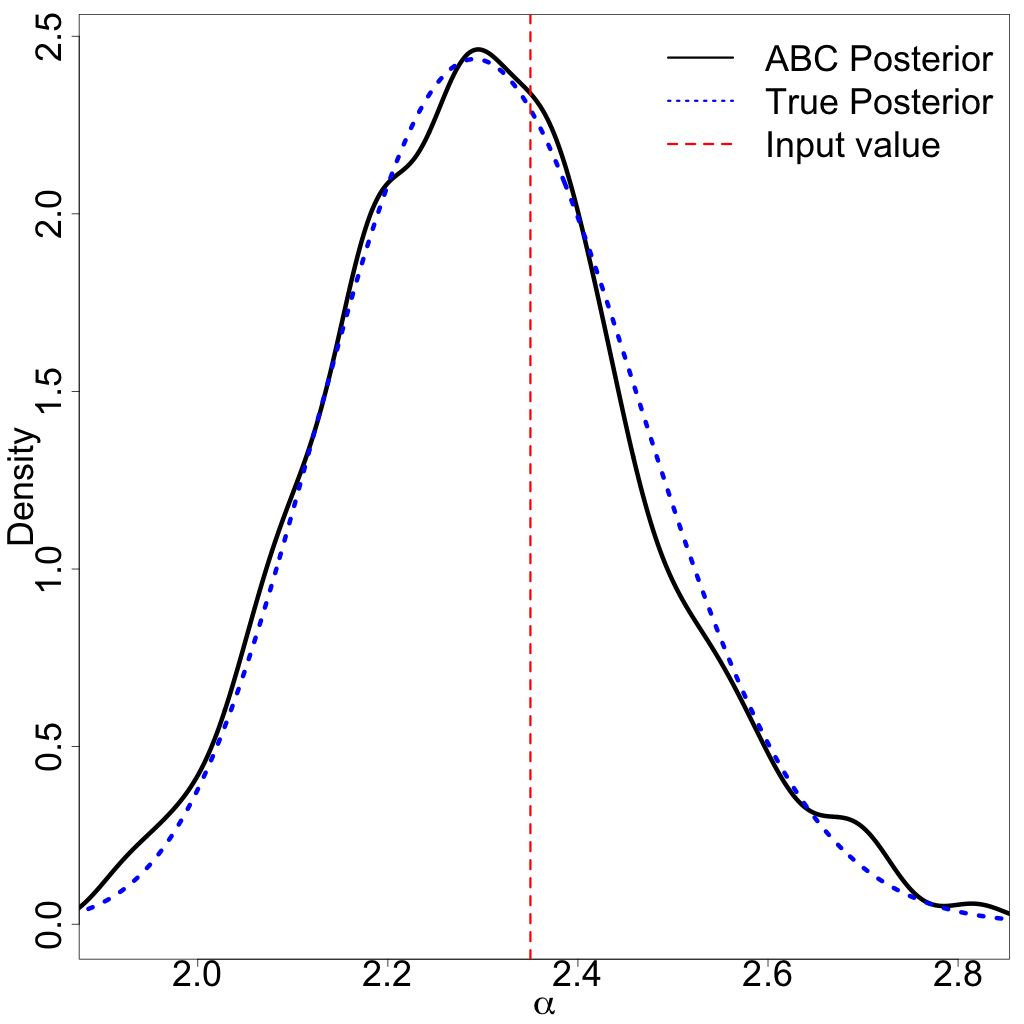
\includegraphics[width=\textwidth]{figures/basic_1_1000_alpha.png}
\caption{Posterior for $\alpha$}\label{subfig:basic_alpha}
\end{subfigure}
\begin{subfigure}{0.32\textwidth}
\centering
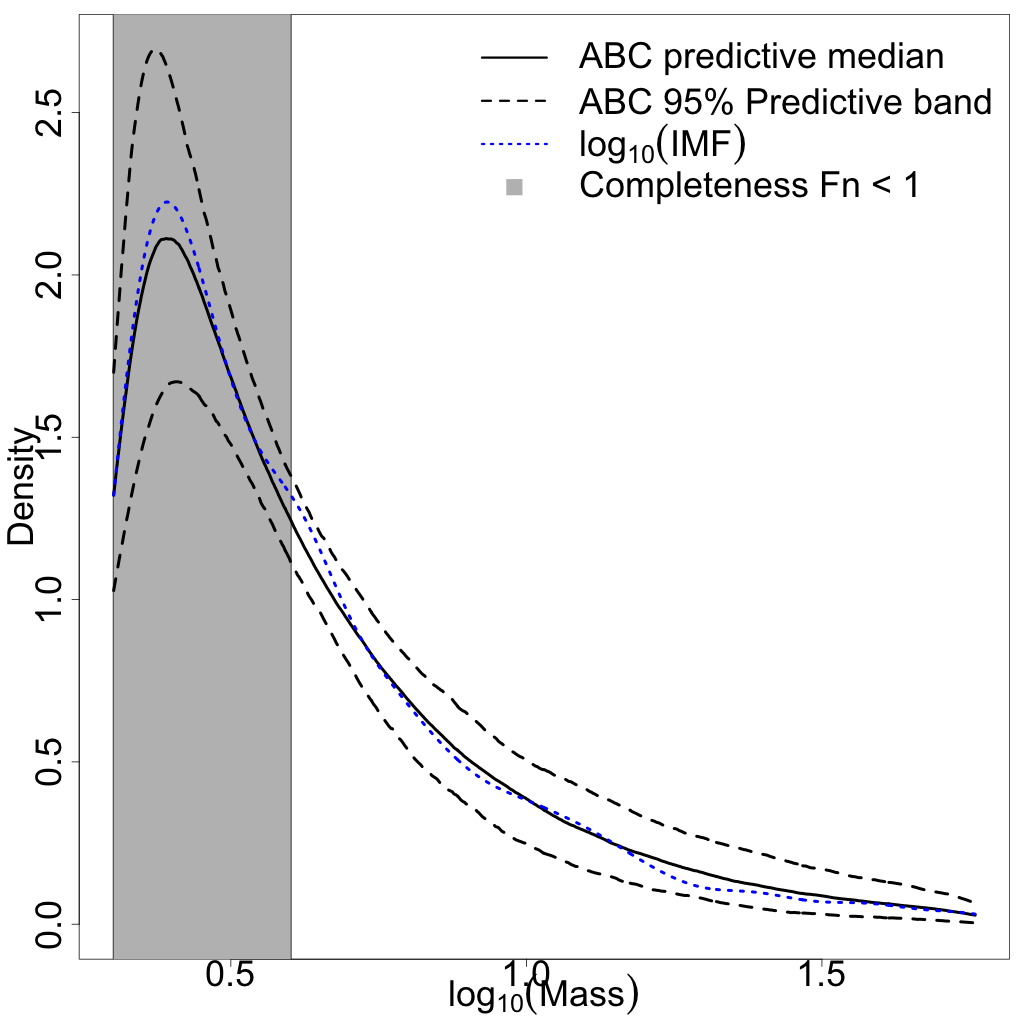
\includegraphics[width=\textwidth]{figures/basic_1_1000_predictive_imf.png}
\caption{Posterior predictive IMF}\label{subfig:basic_imf}
\end{subfigure}
\begin{subfigure}{0.32\textwidth}
\centering
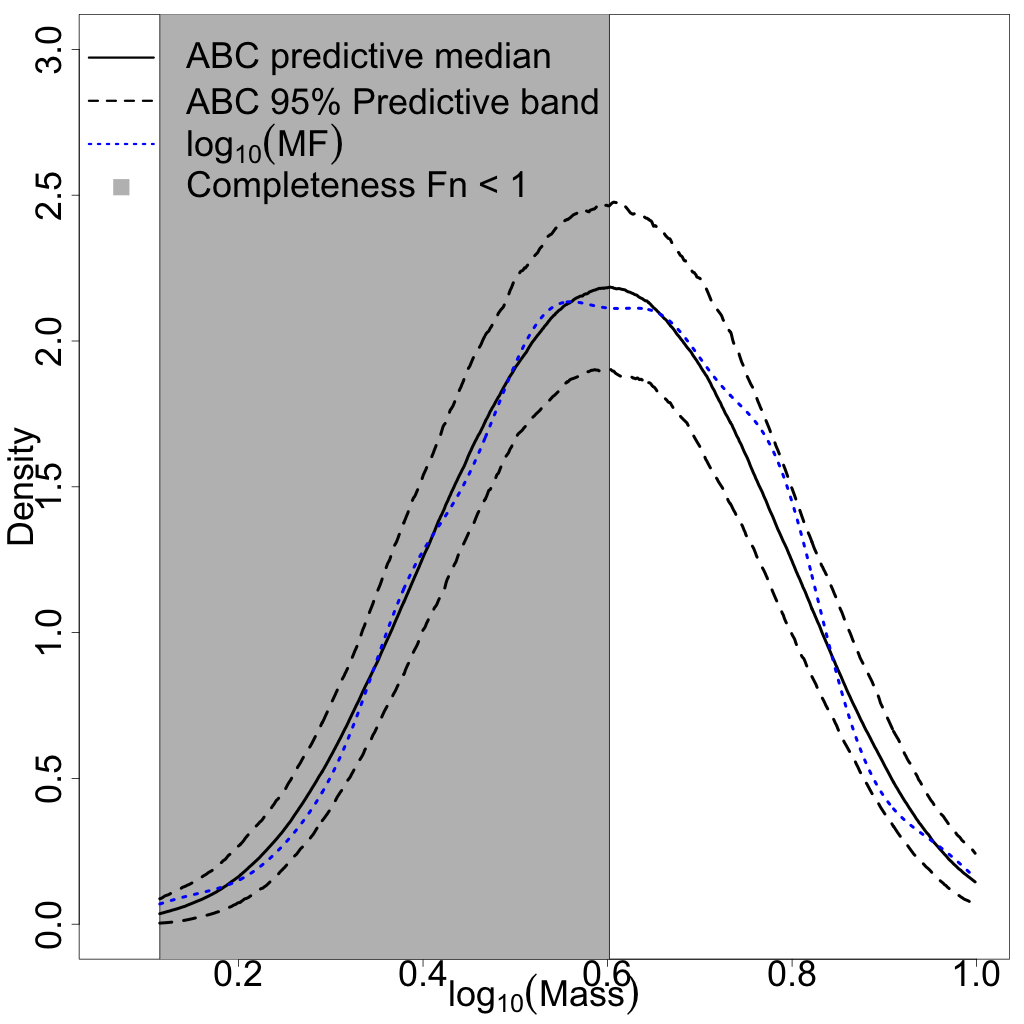
\includegraphics[width=\textwidth]{figures/basic_1_1000_predictive_mf.png}
\caption{Posterior predictive MF}\label{subfig:basic_mf}
\end{subfigure}        
   \caption{Validation of summary statistics with power law model.  (A) The ABC posterior for $\alpha$ (solid black) compared to the true posterior (dotted blue) of Equation~\eqref{eq:simple_posterior} using an input value of 2.35 (dashed vertical red).  (B) The median of the posterior predictive IMF (solid black) with a corresponding 95\% point-wise predictive band (dashed black) compared to the true IMF (blue dotted) which was simulated dataset before aging, completeness, or uncertainty were applied, and the gray shaded region indicates where the completeness function was less than 1.  (C) The median of the posterior predictive MF (solid black) with a corresponding 95\% point-wise predictive band (dashed black) compared to the observed MF (dotted blue) which was the simulated dataset after aging, completeness, and uncertainty were applied.  For the posterior predictive IMF, 1000 draws were made from the ABC posterior of (A) and then 1000 cluster samples were drawn from the power law simulation model.  For the posterior predictive MF, the 1000 cluster samples used for (B) were then put through the forward model to apply the aging, completeness, and measurement error effects.
} \label{fig:abc_simple}
\end{figure}


%\section{Appendix section}\label{app}
%
%XXX
%
%\subsection{Appendix subsection}
%
%XXX
%
%Sample of cross-reference to the formula \ref{path} in Appendix \ref{app}.

\section*{Acknowledgements}
The authors thank the reviewers and associate editor for helpful comments that lead to significant improvements of this work.  The authors also benefited from feedback from Ewan Cameron.  Jessi Cisewski and Grant Weller were partially supported by the National Science Foundation under Grant DMS-1043903. 
Chad Schafer was supported by NSF Grant DMS-1106956.  David W. Hogg was partially supported by the NSF (AST-0908357) and the Moore--Sloan Data Science Environment at NYU.
Any opinions, findings, and conclusions or recommendations expressed in this material are those of the authors and do not necessarily reflect the views of the National Science Foundation.



%\begin{supplement}
%\sname{Supplement A}\label{supp:imf}
%\stitle{Proposed Generative Model Examples}
%\slink[url]{http://www.e-publications.org/ims/support/dowload/imsart-ims.zip}
%\sdescription{xxx}
%\end{supplement}



\bibliographystyle{agsm}
\bibliography{imfABC.bib}

\end{document}
